\chapter{数值仿真结果与分析}


\section{模型描述}

本文选取江苏金坛盐矿某一溶腔进行模拟研究,将不规则溶腔模型简化为长轴为70m,短轴为30m的标准椭球体,理论储气约为26.4万方。溶腔中心点位于地下\SI{936.9}{m}处,溶腔顶部埋深\SI{901.9}{m},底部埋深\SI{971.9}{m},溶腔顶部盐岩厚165m,盐岩上部泥岩厚\SI{736.6}{m}。取地表温度为\SI{17}{ \degreeCelsius},温度梯度为\SI{2.24}{\degreeCelsius}/\SI{100}{m},则模型顶端温度(y=-901.9m)温度为\SI{37.1}{\degreeCelsius}(\SI{310.3}{K});模型下端(y=\SI{-971.9}{m})温度为\SI{38.7}{\degreeCelsius}(\SI{311.8}{K}),溶腔中心(y=\SI{-936.1}{m})温度为\SI{37.9}{\degreeCelsius}(\SI{311.0}{K})。

为消除边界对数值模拟的影响,土体模型尺寸应达到洞泾尺寸的\num{6}倍左右,因此建立长度为400m、宽度为400m、高为400m的轴对称模型。模型正视图如图\ref{fig:5-4}所示。模型底部采用位移边界条件,不论何种工况下底部沿水平方向或数值方向都不会发生位移,垂直方向两侧边界施加水平方向上的位移约束。盐岩计算所需参数见第\ref{section:modelparameters}节中表\ref{tab:1}-\ref{tab:3}。

为提高计算效率,将模型简化为1/4对称模型进行有限元计算,网格划分如图\ref{fig:5-4}所示,共计181935单元,193388节点。
 \begin{figure}[ht!]
    \centering
    \subfigure[三维模型示意图]
    {
        \begin{minipage}{8cm}
            \centering
            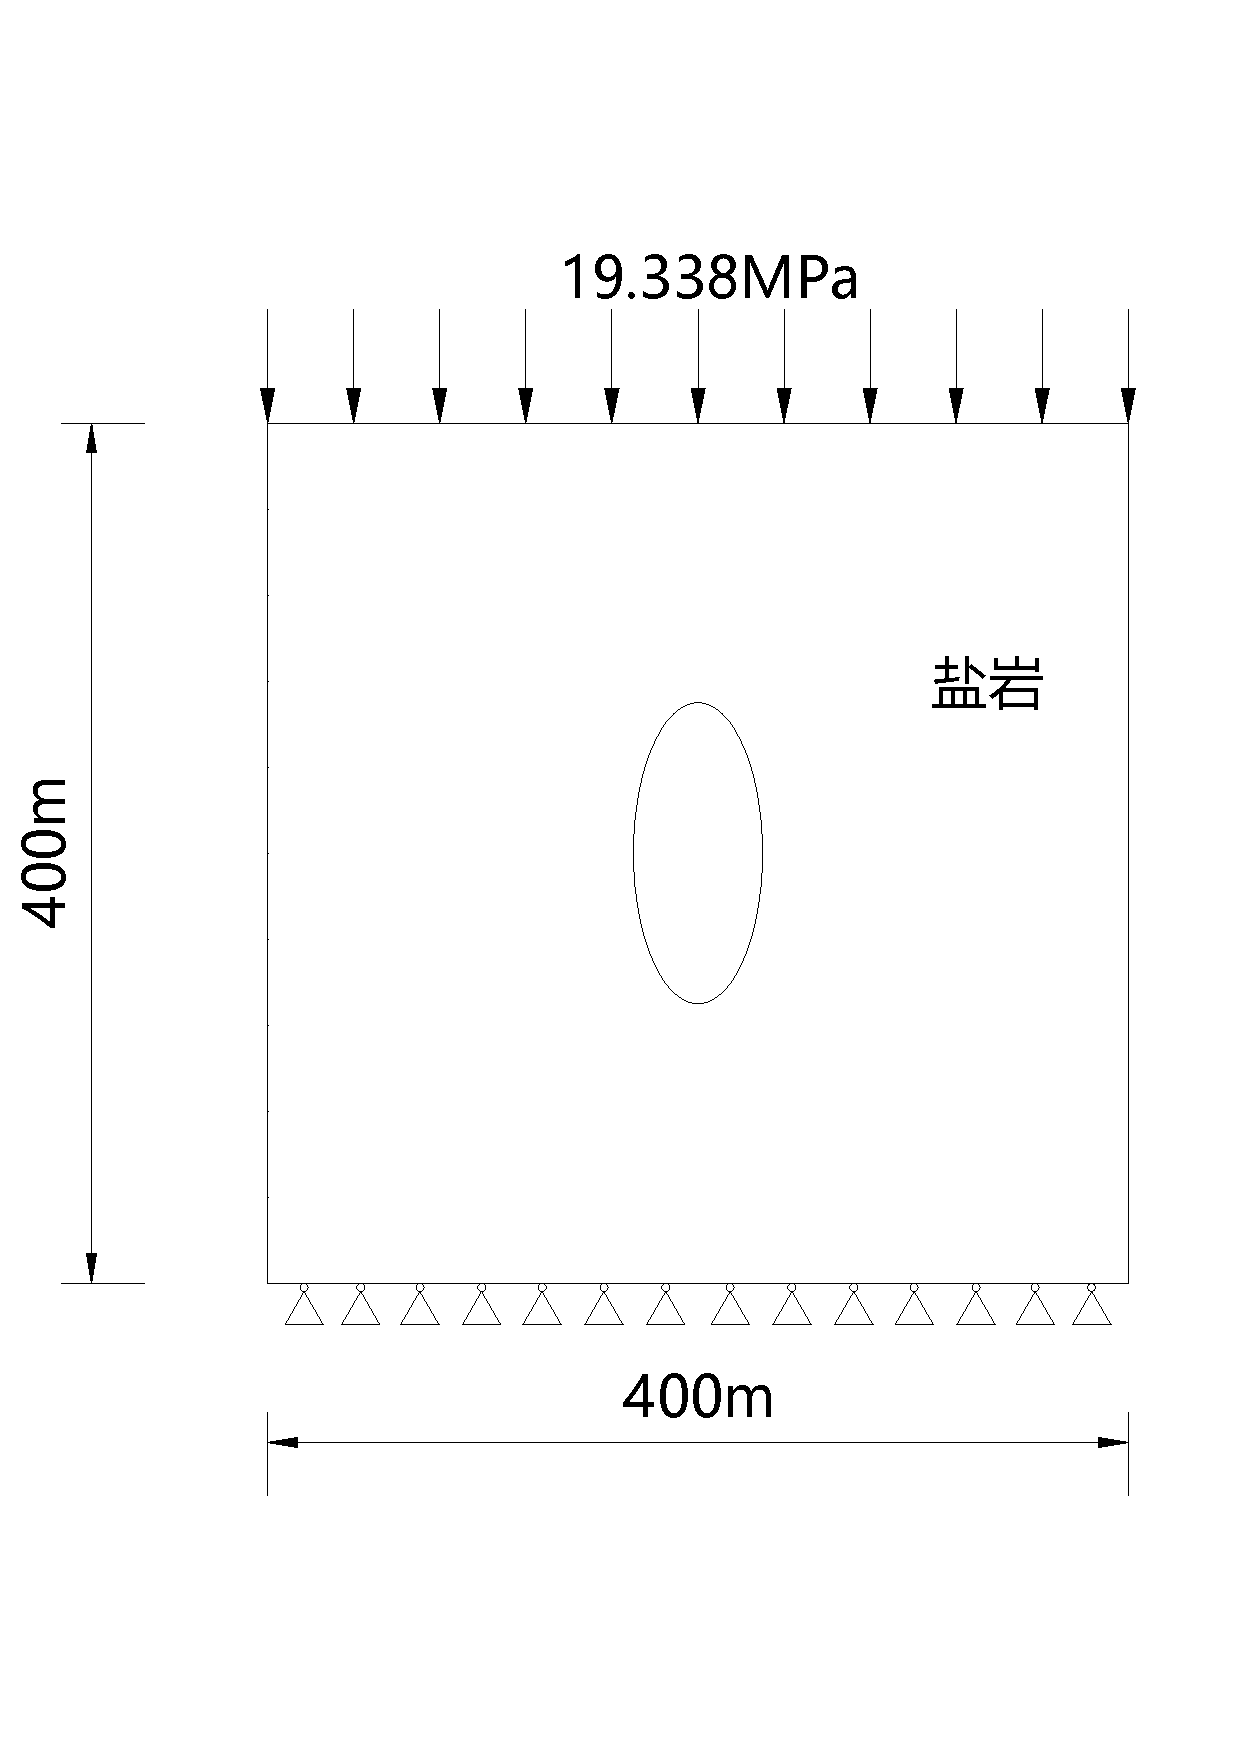
\includegraphics[width=0.85\textwidth]{img/chap5/计算模型图1.15.pdf}
        \end{minipage}
    }
    \subfigure[网格划分图]
    {
        \begin{minipage}{7cm}
            \centering
            \includegraphics[width=0.95\textwidth]{img/chap5/三维模型网格划分图.png}
        \end{minipage}
    }
    \caption{三维模型示意图与网格划分图}
    \label{fig:5-4}
\end{figure}


\section{注采方案}


\subsection{注采时长}
新能源储库的主要是为了调节峰谷时用电,缓解电网压力。电网负载一般由三大产业及居民用电构成,其中第一、第二产业处于全天生产状态,对于电网峰谷变化影响较小。电网的日负载波动主要是由于第三产业及居民日常活动引起。以江苏省为例,忽略季节性影响,民用电高峰时段一般是18时至23时共6小时,用电低谷期一般是1时至6时共计5小时\cite{谈康2016江苏电网负荷特性研究及有序用电管理措施探讨}。如下图\ref{fig:5-2}所示,为波兰2019年3月10日风力发电总量和电网荷载总量与时间关系图\cite{R2021Comprehensive}。图中黄色柱状图表示电网中荷载,蓝色柱状图表示风力发电总量,不难看出用电高峰时期风力发电能力较弱,而用电低谷时期风力发电能力较强。图中曲线表示除去风力发电所需电量,即全天电网荷载峰谷时波动曲线。

根据上述实际的用电情况的资料,制定储气库注采气运行工况如下:用电低谷期0时-7时匀速注气蓄能,用电高峰期7时至24时进行采气发电,以此为一个注采周期,依次循环\cite{谈康2016江苏电网负荷特性研究及有序用电管理措施探讨,R2021Comprehensive}。

\begin{figure}[ht!]
    \centering
    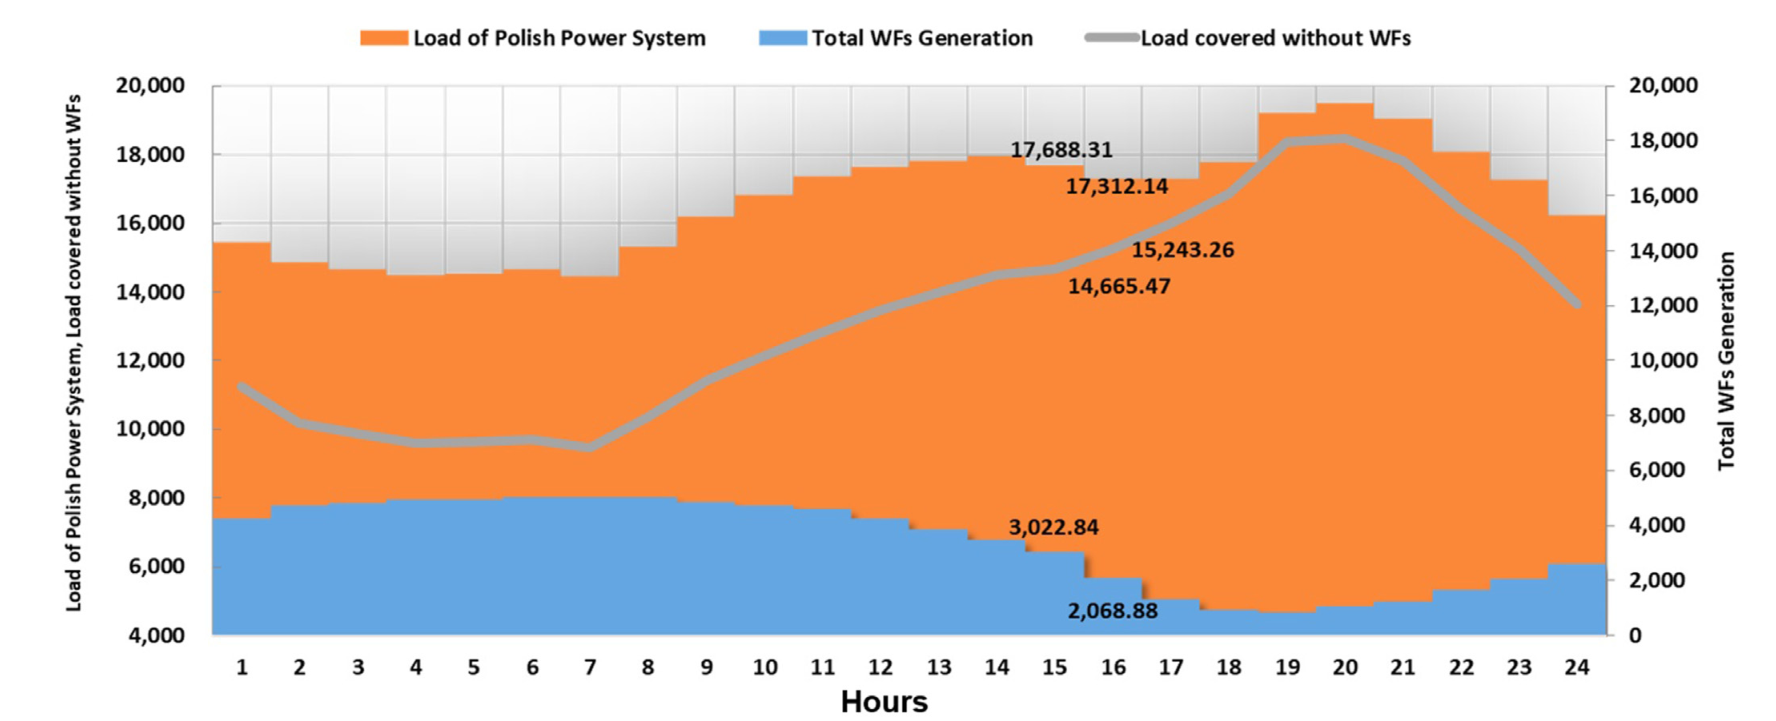
\includegraphics[width=0.95\textwidth]{img/chap5/波兰2019年某一天风力发电和电网总荷载与时间关系图.png}
    \caption{波兰一天内风力发电和电网总荷载与时间关系图\cite{R2021Comprehensive}}
    \label{fig:5-2}
\end{figure}


\subsection{内压变化}
盐岩地下储气库的稳定性包括两个方面,一是造腔施工期间的稳定性,二是保证储气库长期安全运行的稳定性。为保证储气库在设计年限内能安全运行,需对储气库的极限运行压力进行科学合理的设计。

(1)确定最小内压
最小内压的确定主要依据原则:一、顶板稳压原则;二、蠕变控制原则。顶板稳压原则:由于储气过程中腔内压力低于围岩地应力,造腔施工期间的弹性变形以及储库运行期间的蠕变变形会导致腔体顶板下沉。因此最小压力须满足防止顶板过度变形、开裂的变形约束要求。蠕变控制原则:储气库在长期运行的情况下岩石的蠕变会减小储库的有效容积,最小压力越大则一定年限内溶腔收缩率越小,因此最小运行压力须满足体积变化率的要求\cite{梁卫国2008层状盐岩储气库物理力学特性与极限运行压力}。

(2)确定最大内压
最大内压的确定主要依据原则:一、裸井致密原则;二、腔壁致密原则。裸井致密原则:裸井一般位于腔顶部岩层中,与套管靴相连,紧邻盖层,由于水泥与盐岩之间易发生变形不协调,导致气体泄漏。因此腔体内的最大气压必须有所限制,以此保证裸井的致密,避免气体泄漏。腔壁致密原则:
除了裸井之外,整个储库腔体内壁也应该保持致密,即内压应小于或等于最小地应力\cite{梁卫国2008层状盐岩储气库物理力学特性与极限运行压力}。

综合上述确定内压力原则,参考国内外实际储气库、储油库的建设经验,并考虑一定的安全系数,可以认为一般腔体内压的可行范围为上覆岩层压力的30$\%$-75$\%$\cite{王贞硕2020层状盐岩中水平腔压气蓄能储库顶板稳定性研究}。该溶腔上覆岩层压力为22.26MPa,理论允许运行压力范围为6.7MPa-16.7MPa。结合现实际储气库的运行状况的相关经验,拟定该储气库的运行压力上限为14MPa,运行压力下限为8MPa。

\subsection{温度变化}
根据热力学定律及理想气体方程,气体在压缩过程中会导致温度上升,并在注入腔体内后与围岩发生热量交换。图~\ref{fig:5-5}为韩中合参考Huntorf电站,对储气库系统模型求解结果\cite{韩中合2017储气室热力学特性对}。

如图(a)不同对流换热系数时储气室温度变化中显示,当对流换热系数h=0,即不考虑气体与围岩之间的热量交换时,初始气体温度为\SI{323}{K},注气阶段气体温度上升较快,近似呈线性变化,注气阶段结束后气体温度为\SI{378}{K};采气阶段气体温度也呈线性下降。直到采气阶段结束时,储气库压力恢复至初始气压,而气体温度略高于初始温度。随着$h$的增大,气体与围岩的热交换明显,气体温度上升和下降都逐渐缓慢。当h足够大时候,气体温度逐渐趋于平缓。当$h=\infty$,即恒温模型下,储气库运行各个阶段温度都保持不变,内压升高缓慢,系统运行时间最长。

参考该文献中储气库在运行过程中温度和压力随时间变化情况,制定本文中不考虑气体与围岩热量交换时储气库的运行工况。


\begin{figure}[ht!]
    \centering
    \subfigure[不同对流换热系数时储气室温度变化]
    {
        \begin{minipage}{7cm}
            \centering
            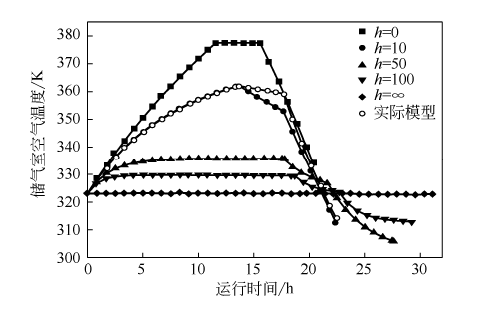
\includegraphics[width=0.95\textwidth]{img/chap5/不同对流换热系数时储气室温度变化.png}
        \end{minipage}
    }
    \subfigure[不同对流换热系数时储气室压力变化]
    {
        \begin{minipage}{7cm}
            \centering
            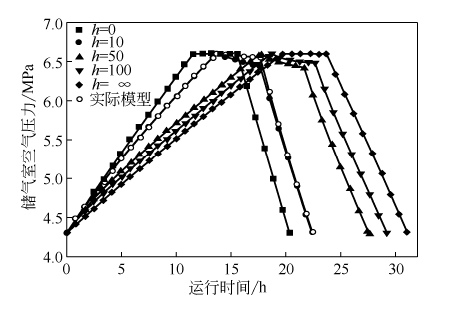
\includegraphics[width=0.95\textwidth]{img/chap5/不同对流换热系数时储气室压力变化.png}
        \end{minipage}
    }
    \caption{不同对流换热系数时储气室温度、压力变化\cite{韩中合2017储气室热力学特性对}}
    \label{fig:5-5}
\end{figure}


\section{新能源储库运行工况设置}
\subsection{考虑热力耦合}
综合上述注采周期、内压变化、注采温度变化分析,并结合江苏金坛地区已建储库的实际运作模式,拟定如图~\ref{fig:5-1}的新能源储库运行工况,以24小时为一个注采周期,\numrange{0}{7}小时注气,\numrange{7}{24}小时采气,如此循环往复。储库运行压力上限设定为\SI{14}{MPa},下限设定为\SI{8}{MPa}。计算得到气体最高温度为\SI{378}{K},最低温度为\SI{323}{K}。

\begin{figure}[ht!]
    \centering
    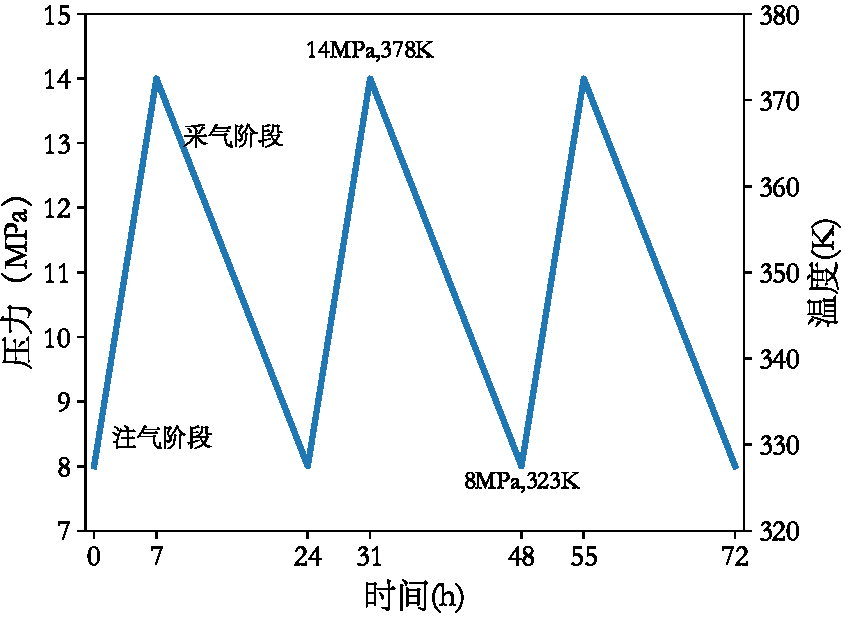
\includegraphics[width=0.55\textwidth]{img/chap5/储气库模拟运行工况.pdf}
    \caption{新能源储库考虑耦合模拟运行工况}
    \label{fig:5-1}
\end{figure}

% 实现计算脚本中储库运行工况设置如下。
% \begin{lstlisting}[breaklines,language=XML]
% <parameter>
%         <name>internal_pressure_value</name>
%         <type>Function</type>
%         <expression>(t%1>7.0/24.0? 144.0e6/17*(t%1)-280/17: -144.0e6/7*(t%1)-8.0e6)</expression>
% </parameter>
% <parameter>
%         <name>internal_bc_value</name>
%         <type>Function</type>
%         <expression>(t%1>7.0/24.0? -1320.0/17*(t%1)+6811/17: 1320.0/7*(t%1)+323)</expression>
% </parameter>
% \end{lstlisting}
% 其中internal\_pressure\_value为压力变化,压力单位为Pa,internal\_bc\_value为温度变化,温度单位为\si{K},时间$t$单位为\si{d}。

\subsection{不考虑热力耦合}
不考虑热力耦合的情况下,模拟新能源储库运行工况如图~\ref{fig:5-16}所示。周期压力的设置与考虑热力耦合的情况相同,参照前文对模型条件的描述,气体温度与溶腔中心温度相同,拟定为\SI{323.0}{K},且认为在气体压缩和释放过程中不发生温度变化。

\begin{figure}[ht!]
    \centering
    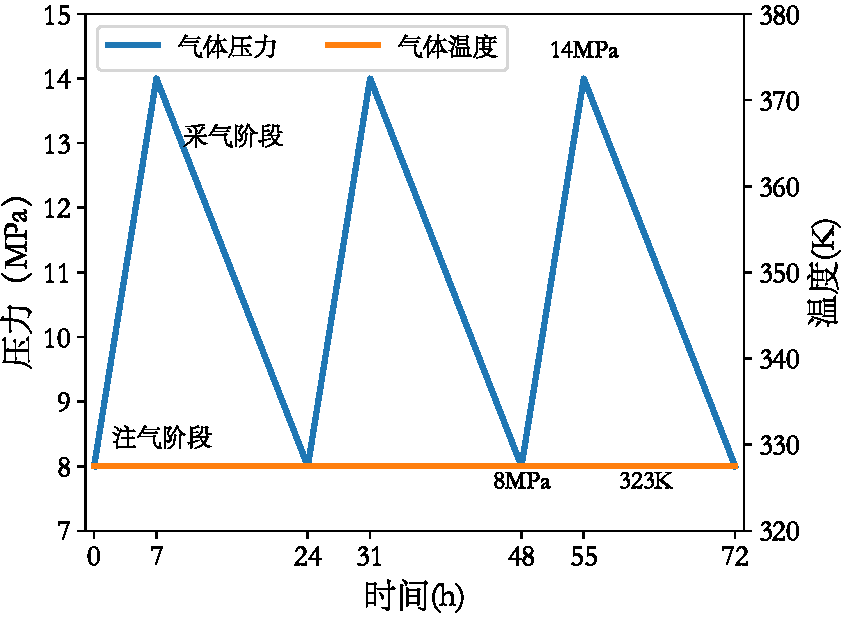
\includegraphics[width=0.55\textwidth]{img/chap5/压气蓄能库运行工况无耦合.pdf}
    \caption{新能源储库无耦合模拟运行工况}
    \label{fig:5-16}
\end{figure}

% 根据拟定的运行工况,计算代码中边界条件设置如下。
% \begin{lstlisting}[breaklines,language=XML]

% <parameter>
%     <name>internal_pressure_value</name>
%     <type>Function</type>
%     <expression>(t%1>7.0/24.0? 144.0e6/17*(t%1)-280e6/17: -144.0e6/7*(t%1)-8.0e6)</expression>
% </parameter>
% <parameter>
%     <name>internal_bc_value</name>
%     <type>Constant</type>
% <value>323.0</value>
% </parameter>
% \end{lstlisting}

\section{传统能源储库运行工况设置}

\subsection{考虑热力耦合}
利用地下盐穴作为传统能源储库(如:天然气储库),能够有效的保证供需平衡,维持供给的可靠性、连续性,避免出现供给不均匀的情况。因此相较于新能源储库,传统能源储库的循环注采周期较长,参考谭贤君等\cite{陈卫忠2007盐岩非线性蠕变损伤本构模型及其工程应用,盐岩储气库温度}在盐岩储气库温度-渗流-应力-损伤耦合模型研究、陈卫忠等在盐岩非线性蠕变损伤本构模型及其工程应用中的模型设置,并结合江苏金坛地区的天然气使用情况拟定储库运行工况。一年中,0-3月份为恒定低压阶段,0-6月份为注气阶段,6-9月份为恒定高压阶段,9-12月份为采气阶段。腔内气体最高压力为\SI{14}{Mpa},最低压力为\SI{8}{Mpa},最高温度为\SI{378}{K},最低温度为\SI{323}{K}。具体运行工况如图~\ref{fig:5_10}所示,以一年为一个循环周期,运行时间为10年进行模拟计算。
\begin{figure}[ht!]
    \centering
    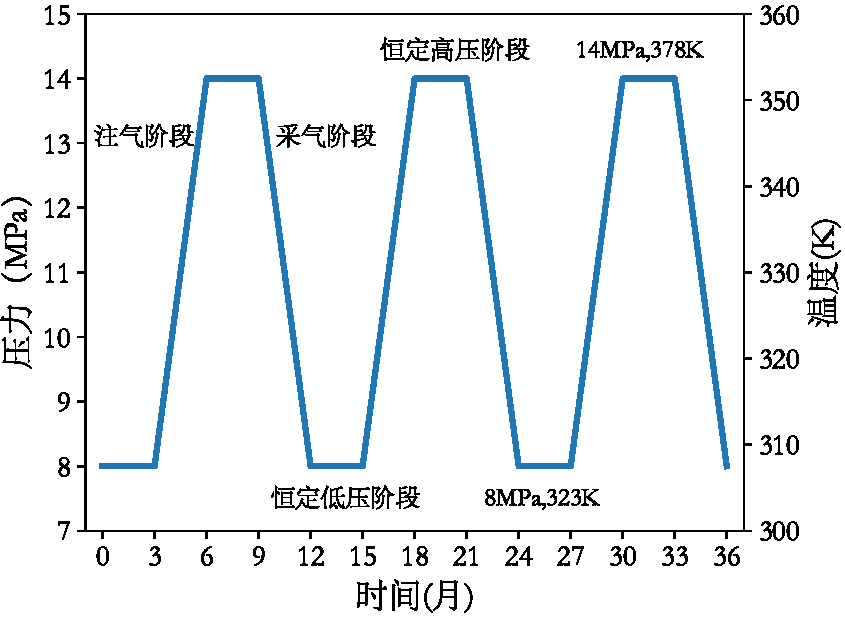
\includegraphics[width=0.55\textwidth]{img/chap5/10年天然气储库运行工况.pdf}
    \caption{传统能源储库考虑耦合模拟运行工况}
    \label{fig:5_10}
\end{figure}
\begin{figure}[ht!]
    \centering
    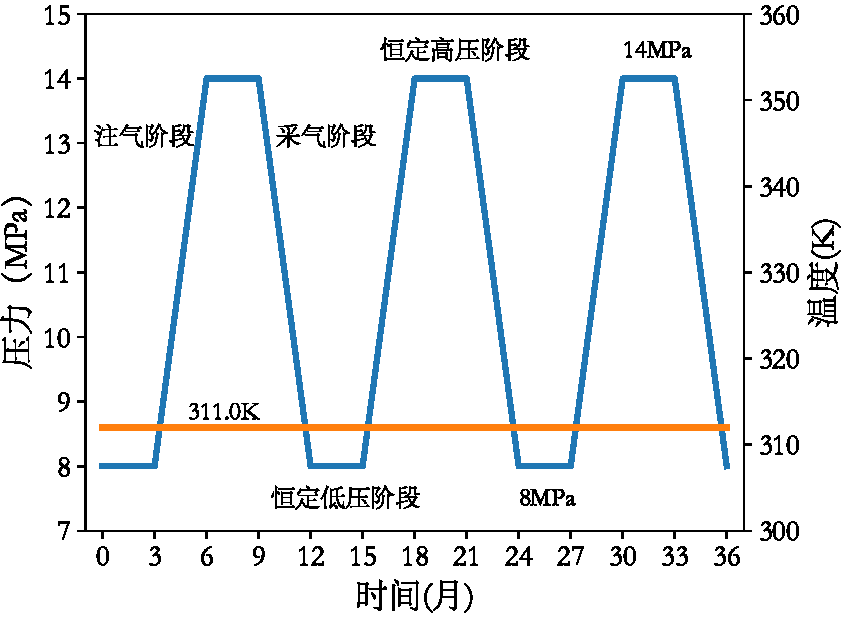
\includegraphics[width=0.55\textwidth]{img/chap5/储气库无耦合.pdf}
    \caption{传统能源储库无耦合模拟运行工况}
    \label{fig:5_11}
\end{figure}
% 根据拟定的天然气储库实际运行工况,计算代码中循环边界条件设置如下。
% \begin{lstlisting}[breaklines,language=XML]
% <parameter>
%     <name>internal_pressure_value</name>
%     <type>Function</type>
%     <expression>(t%360>180? (t%360>270? 1.0e6/15*(t%360)-32.0e6: -14.0e6):(t%360>90? -1.0e6/15*(t%360)-2.0e6: -8.0e6))</expression>
% </parameter>
% <parameter>
%     <name>internal_bc_value</name>
%     <type>Function</type>
%     <expression>(t%360>180? (t%360>270? -11/18*(t%360)+543: 378):(t%360>90? 11/18*(t%360)+268: 323))</expression>
% </parameter>
% \end{lstlisting}


\subsection{不考虑热力耦合}
不考虑热力耦合的情况下,模拟实际储库运行进行计算。周期压力的设置与考虑热力耦合的情况相同,参照前文对模型条件的描述,气体温度与溶腔中心温度相同,拟定为\SI{311.0}{K},且认为在气体压缩和释放过程中不发生温度变化和热量交换。实际运行过程中,气体压力和温度的变化如图~\ref{fig:5_11}所示。



% 根据拟定的天然气储库实际运行工况,计算代码中循环边界条件设置如下。

% \begin{lstlisting}[breaklines,language=XML]
% <parameter>
%     <name>internal_pressure_value</name>
%     <type>Function</type>
%     <expression>(t%360>180? (t%360>270? 1.0e6/15*(t%360)-32.0e6: -14.0e6):(t%360>90? -1.0e6/15*(t%360)-2.0e6: -8.0e6))</expression>
% </parameter>
% <parameter>
%     <name>internal_bc_value</name>
%     <type>Constant</type>
%     <value>311.0</value>
% </parameter>
% \end{lstlisting}

\section{计算工况汇总}
从上述两种储库实际工况的分析中可以看出,新能源储库和传统能源储库工作时压力范围、温度范围大致相同,而循环周期差异较大。因此在长期模拟过程中,拟定两种储库的压力变化范围和温度变化范围不同,设置不同循环周期,以此比较两者长期运行过程中的稳定性。拟定工况汇总于表\ref{tab:5_10}。

\begin{table}[ht!]\small
    \centering
    \begin{tabular}{M{0.1\textwidth}M{0.1\textwidth}M{0.1\textwidth}M{0.06\textwidth}M{0.1\textwidth}M{0.1\textwidth}M{0.1\textwidth}M{0.1\textwidth}}
        \toprule
        计算工况 &储库类型&热力耦合 & 循环周期(d)& 最低内压 (MPa) & 最高内压(MPa) &最低温度 (K) & 最高温度(K) \\
        \midrule
        工况一 &新能源储库  &是  &1   &8    &14    & 323     & 378   \\
        \midrule
        工况二  &新能源储库   &否 &1   &8   &14    & 323     & 323  \\ 
         \midrule
        工况三  &传统能源储库   &是 &360  &8   &14    & 323  & 378  \\ 
         \midrule
        工况四 &传统能源储库   &否 &360  &8   &14    & 323    & 323  \\ \bottomrule
    \end{tabular}
    \caption{计算工况表}
    \label{tab:5_10}
\end{table}


\section{模型验证}
\subsection{模拟储库运营2天计算校验}

由于模型算量大,计算机算力有限,因此实际计算前,先进行代码可行性与合理性验证。将盐岩蠕变本构设置为弹性模型,进行运行测试。经理论分析,若围岩变形符合胡克定律,在周期荷载的作用下,则位移会产生周期性变化,且位移变化周期与荷载变化周期相同。

% 测试过程本构模型、参数修改代码如下。

% \begin{lstlisting}[language=XML]
% <constitutive_relation>
%     <type>LinearElasticIsotropic</type>
%     <youngs_modulus>E</youngs_modulus>
%     <poissons_ratio>nu</poissons_ratio>
% </constitutive_relation>
% \end{lstlisting}

% \begin{lstlisting}[language=XML]
% <parameter>
%     <name>E</name>
%     <type>Constant</type>
%     <value>18.0e9</value>
% </parameter>
% <parameter>
%     <name>nu</name>
%     <type>Constant</type>
%     <value>0.27</value>
% </parameter>
% \end{lstlisting}
% 测试采用弹性模型完成,其中E为杨氏模量,nu为泊松比,取值参照表\ref{tab:2}。

按照上述弹性本构模型试算文件进行计算,得到试算结果。取腔体围岩典型部位的三个点,绘制位移与时间的关系曲线如图~\ref{fig:E}所示。围岩位移随时间发生周期性变化且周期为\SI{1}{d},与边界条件的变化周期相同。可验证循环注采边界代码可行,且运行结果符合理论分析,可以对实际工程进行模拟计算。
\begin{figure}[ht!]
    \centering
    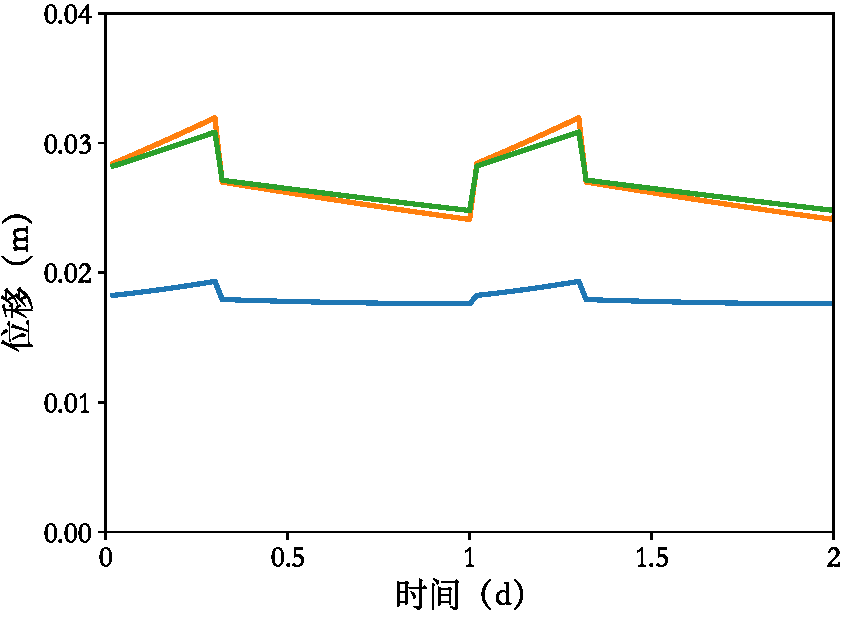
\includegraphics[width=0.55\textwidth]{img/chap5/弹性本构测试结果.pdf}
    \caption{弹性本构模型位移与时间关系曲线}
    \label{fig:E}
\end{figure}

\subsection{模拟储库运营7天结果分析}

\subsubsection{位移}
围岩位移云图如图~\ref{fig:dispalcement}所示,图~\ref{fig:dispalcement1d}为运行\SI{1}{d}后位移云图,图~\ref{fig:dispalcement7d}为运行\SI{7}{d}后位移云图。\SI{1}{d}与\SI{7}{d}整体蠕变趋势相同,腔顶下沉,腔底鼓起,腰部向内收缩。周围岩石因受到地应力的作用而向腔体内部收缩,主要集中于腔体腰部。由于地应力的不断增大,越接近腔底储库内压力与地应力差值越大,因此产生的位移越大。

\begin{figure}[ht!]
    \centering
    \subfigure[运行\SI{1}{d}围岩位移云图]
    {
        \begin{minipage}{7cm}
            \centering
            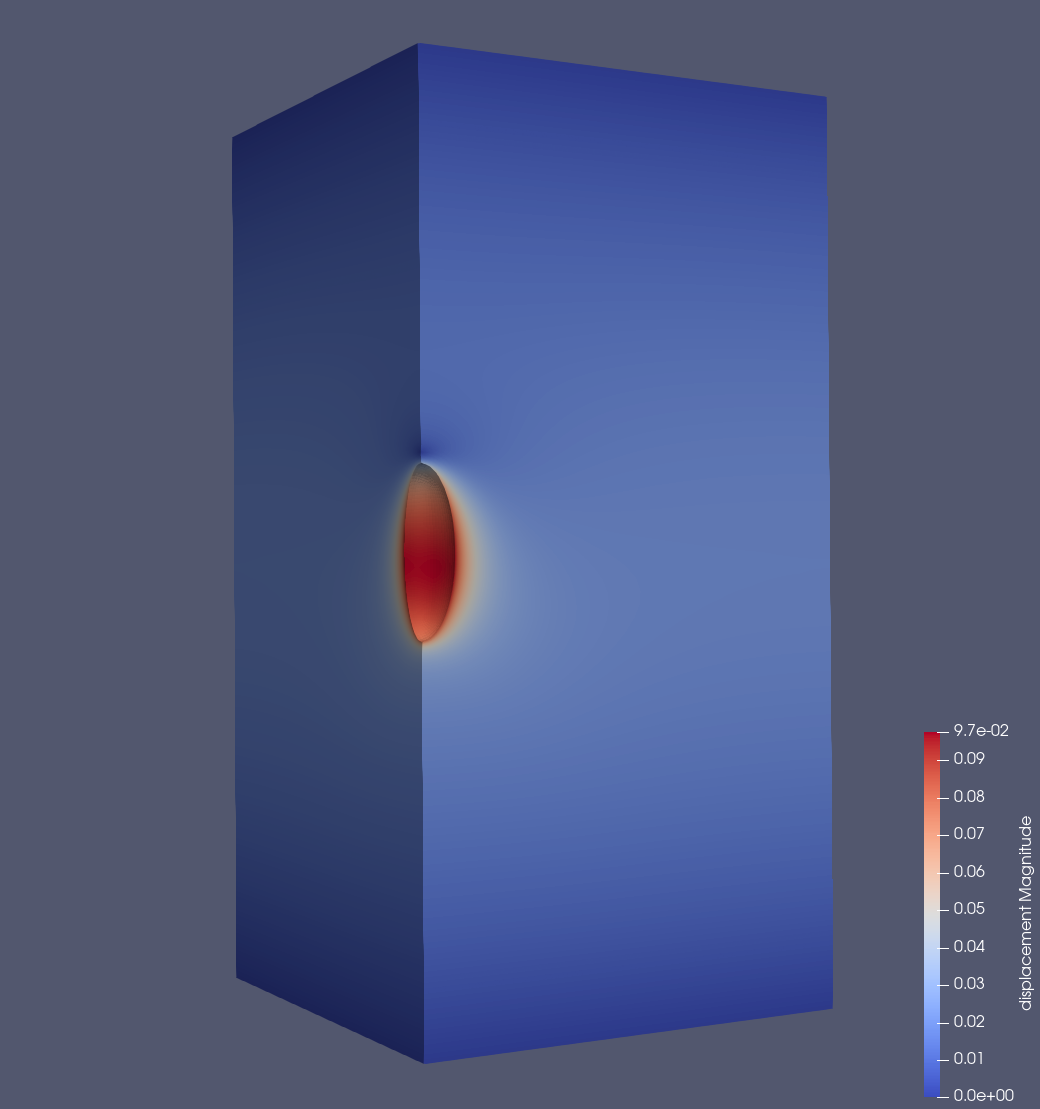
\includegraphics[width=0.95\textwidth]{img/chap5/1d位移云图.png}
        \end{minipage}
        \label{fig:dispalcement1d}
    }
    \subfigure[运行\SI{7}{d}围岩位移云图]
    {
        \begin{minipage}{7cm}
            \centering
            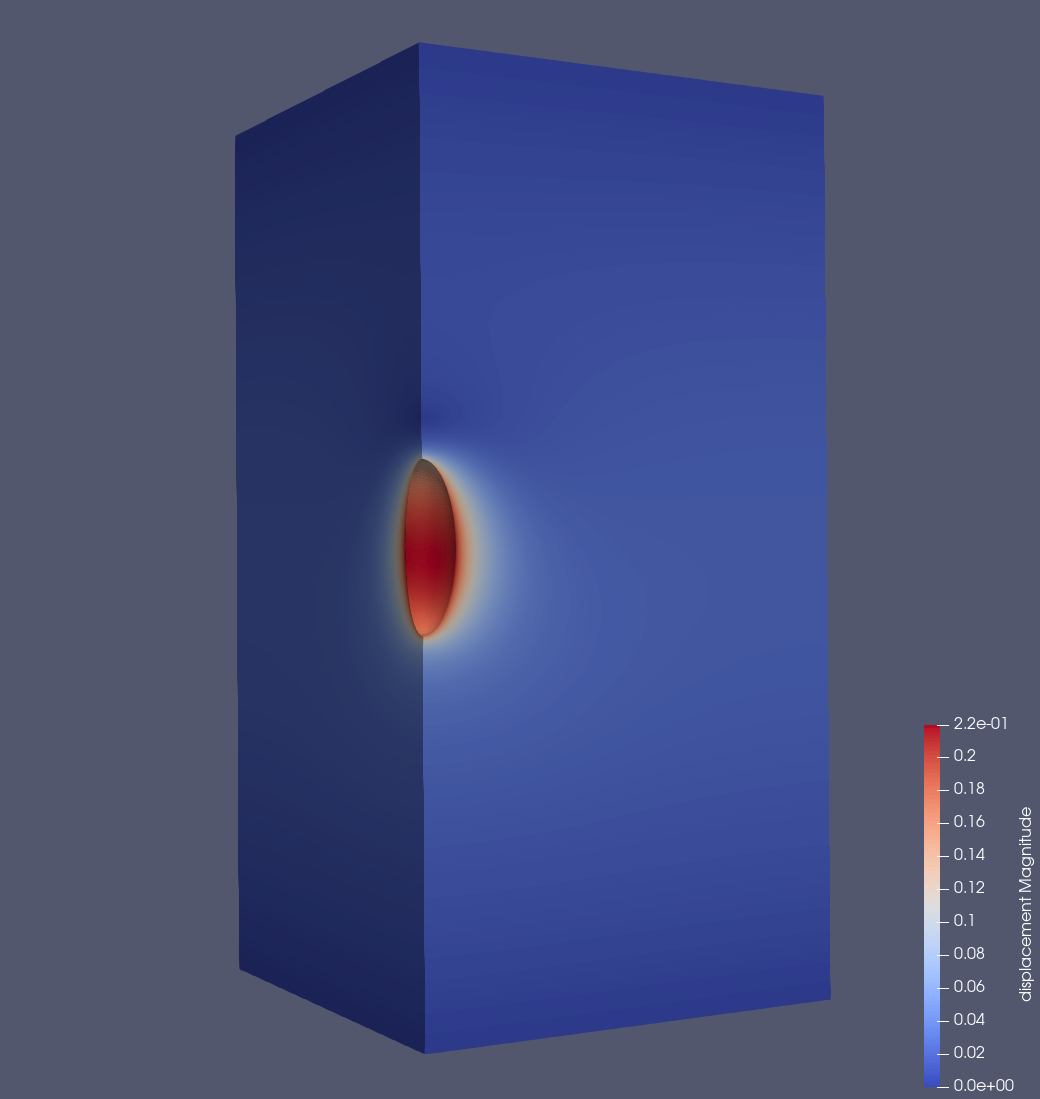
\includegraphics[width=0.95\textwidth]{img/chap5/7d位移云图.png}
        \end{minipage}
        \label{fig:dispalcement7d}
    }
    \caption{\SI{1}{d}、\SI{7}{d}围岩位移云图(单位:m)}
    \label{fig:dispalcement}
\end{figure}

腔体底部最大位移为\SI{0.174}{m},腔体顶部最大位移为\SI{0.123}{m}。由于腔体呈椭球状,在顶部和底部逐渐收缩,水平方向的应力逐渐相互抵消,因此产生的位移量小于腔体中部。水平应力的相互作用,也会导致围岩挤压而向内收缩,因此应力更大的腔底比腔顶位移大。

图~\ref{fig:7d_displacement_max}为\SI{7}{d}内最大位移与随时间变化情况。经过一个注采周期,即运行\SI{1}{d}后最大位移为\SI{0.097}{m},运行\SI{7}{d}后,最大位移为\SI{0.219}{m}。\SI{7}{d}内最大位移与时间变现出良好的线性关系,根据曲线规律,随着储库运行时间的增加,位移仍会大幅增加。


\begin{figure}[ht!]
    \centering
    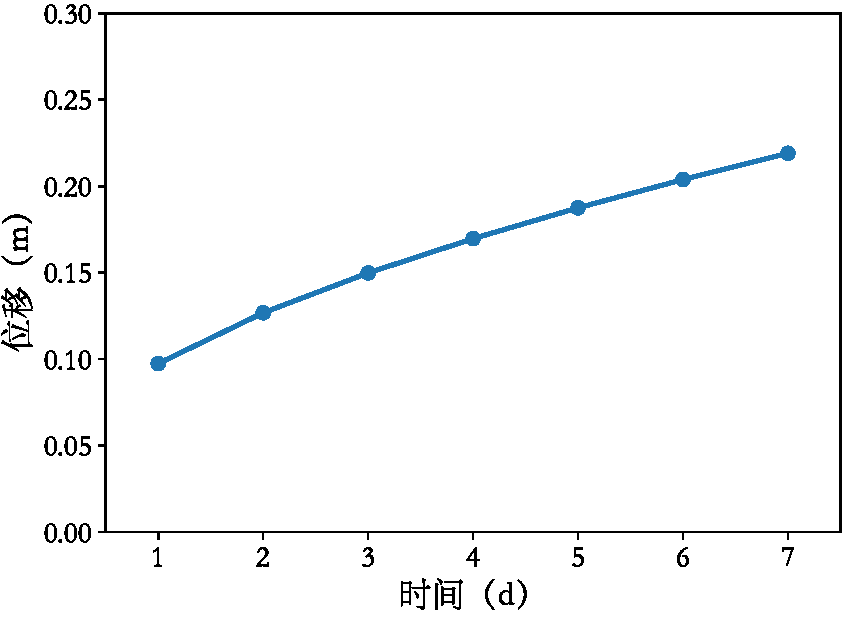
\includegraphics[width=0.55\textwidth]{img/chap5/7d最大位移.pdf}
    \caption{\SI{7}{d}模拟运行最大位移与时间关系曲线}
    \label{fig:7d_displacement_max}
\end{figure}


在腔体上部、中部、下部取三个点,如图~\ref{fig:weizhi}所示,分别作出这三个点位移随着时间变化关系如图~\ref{fig:7d_displacement_A}所示。图像显示,在洞内压力周期性变化时,位移也成周期性变化,且变化周期与压力变化周期一致。

\begin{figure}[ht!]
    \centering
    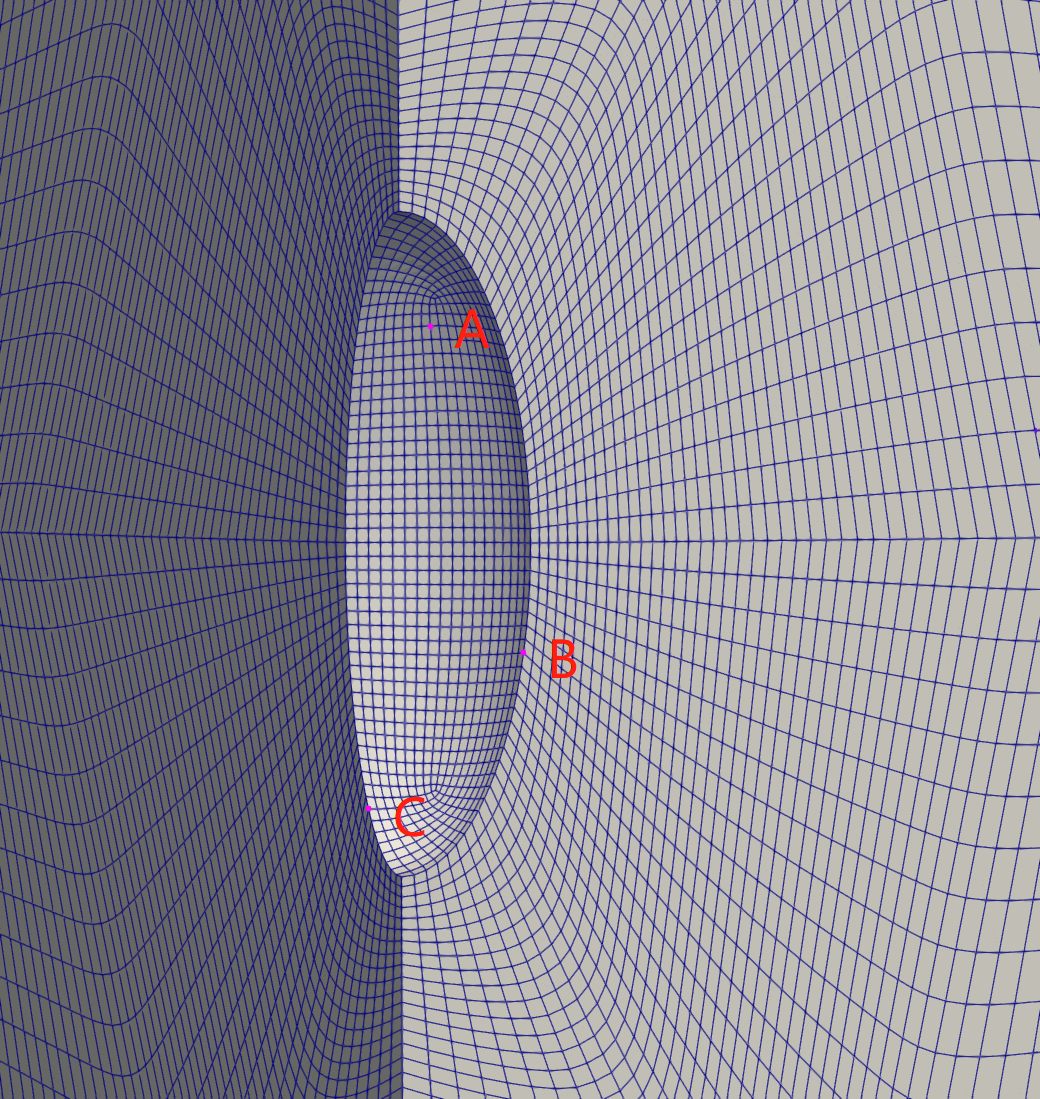
\includegraphics[width=0.5\textwidth]{img/chap5/三点位移.png}
    \caption{A点、B点、C点位置}
    \label{fig:weizhi}
\end{figure}


\begin{figure}[ht!]
    \centering
    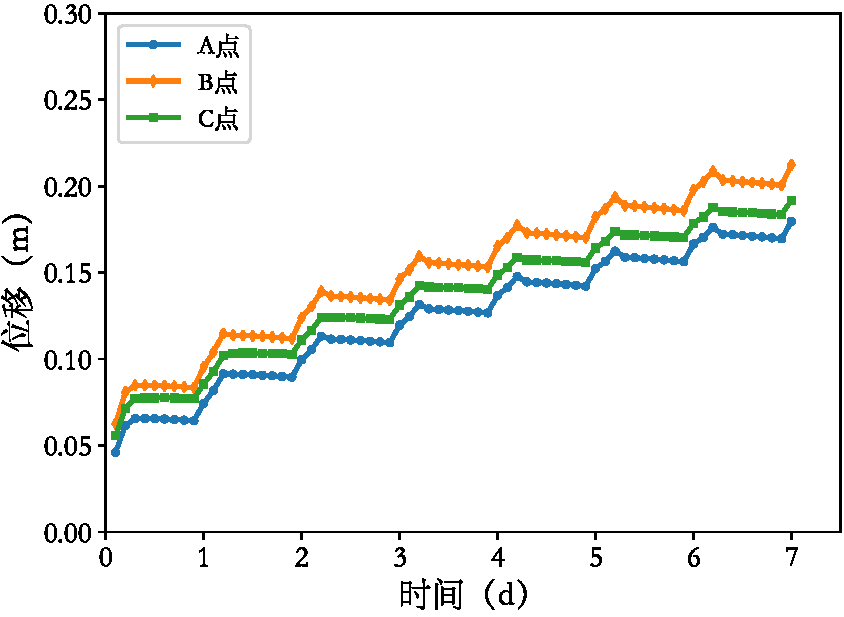
\includegraphics[width=0.55\textwidth]{img/chap5/三点位移随时间变化曲线.pdf}
    \caption{\SI{7}{d}内A点、B点、C点位移随时间变化曲线}
    \label{fig:7d_displacement_A}
\end{figure}

\subsubsection{应力}
围岩应力云图如图~\ref{fig:sigma}所示,图~\ref{fig:sigma1d}为运行\SI{1}{d}后应力云图,图~\ref{fig:sigma7d}为运行\SI{7}{d}后应力云图。应力集中于腔腰部位,运行\SI{7}{d}后,腔腰部最大应力可达\SI{164.9}{MPa},腔顶和腔底部分最大应力则相对较小,在\SI{20}{MPa}-\SI{50}{MPa}之间。
\begin{figure}[ht!]
    \centering

    \subfigure[运行\SI{1}{d}围岩应力云图]
    {
        \begin{minipage}{7cm}
            \centering
            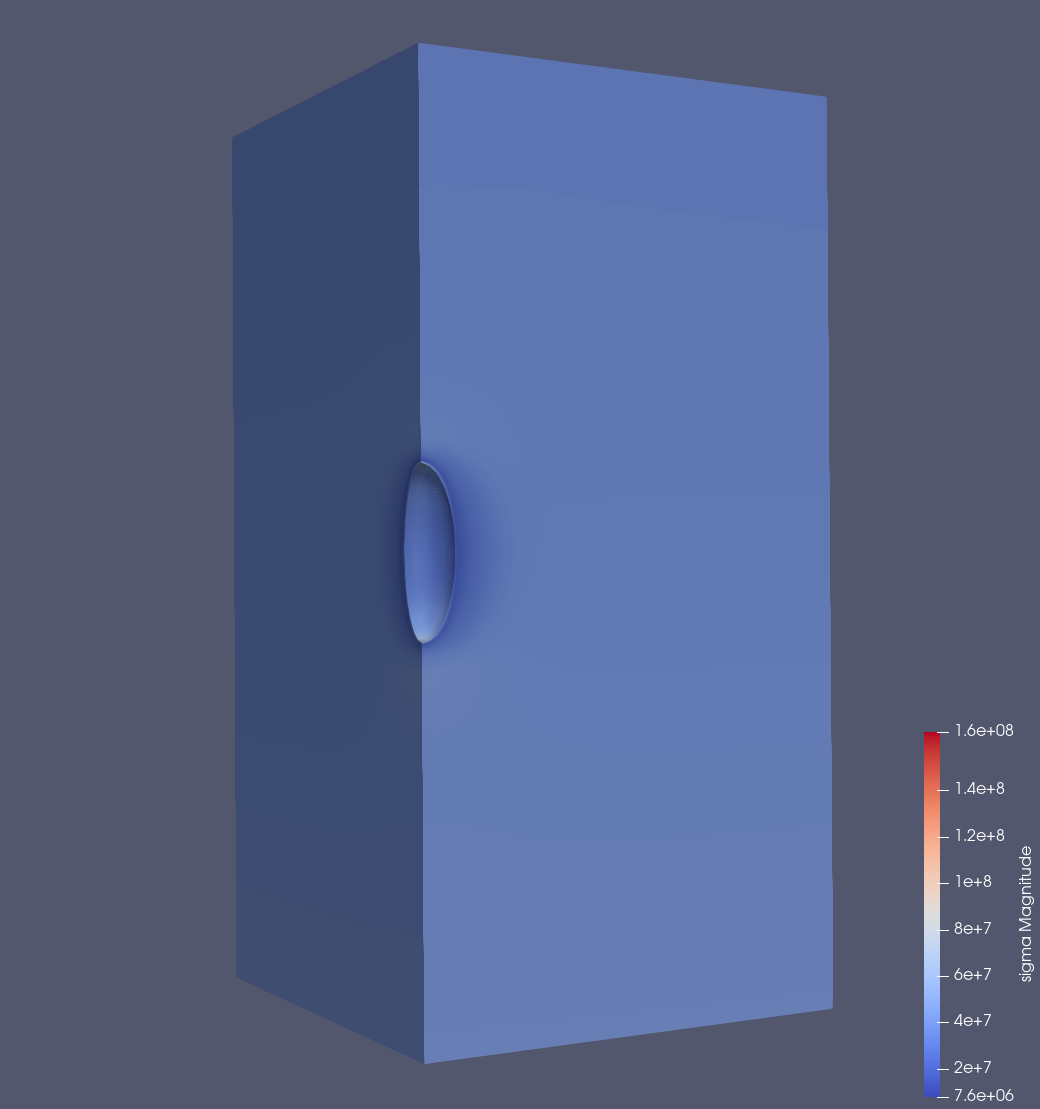
\includegraphics[width=0.95\textwidth]{img/chap5/1d应力云图.png}
        \end{minipage}
        \label{fig:sigma1d}
    }
    \subfigure[运行\SI{7}{d}围岩应力云图]
    {
        \begin{minipage}{7cm}
            \centering
            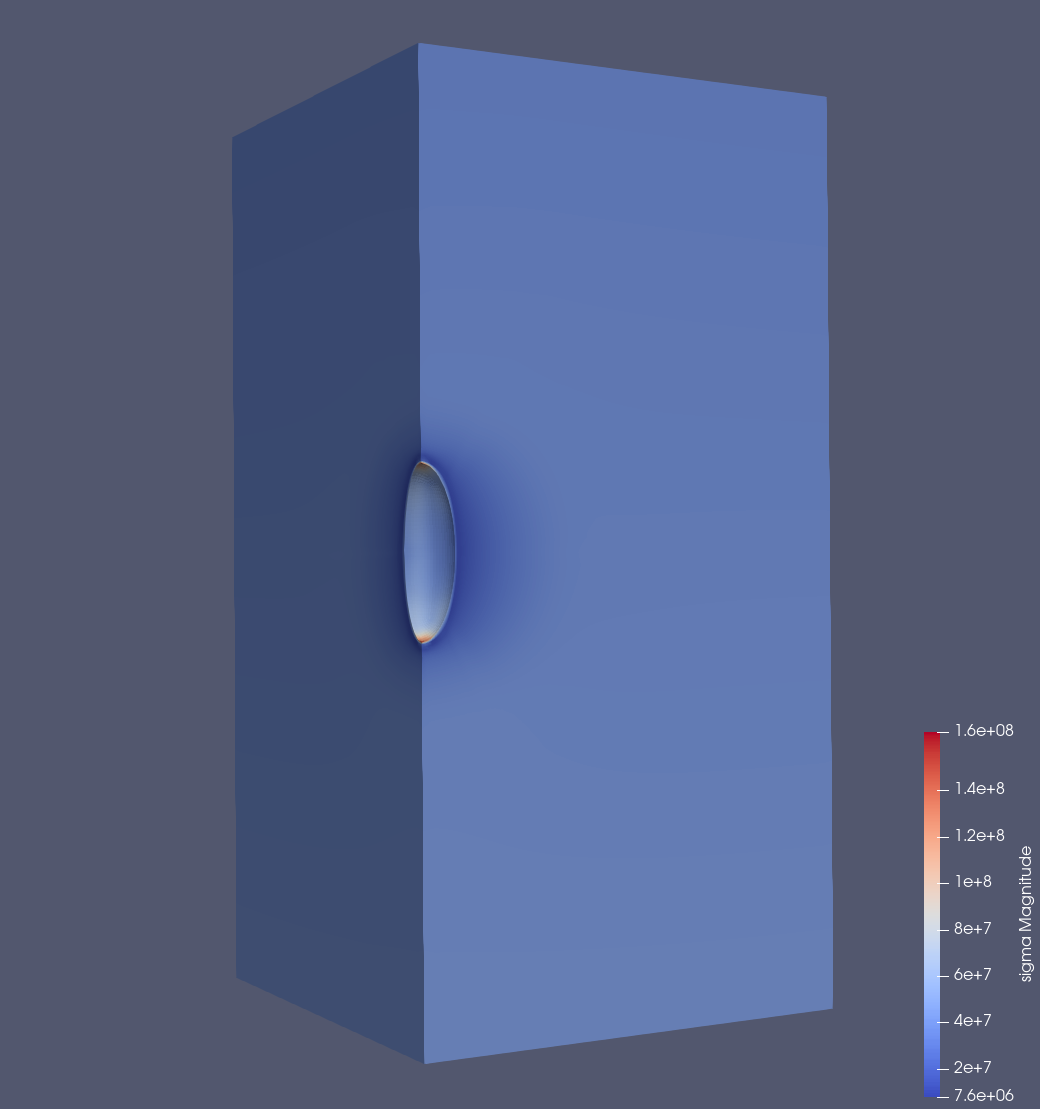
\includegraphics[width=0.95\textwidth]{img/chap5/7d应力云图.png}
        \end{minipage}
        \label{fig:sigma7d}
    }
    \caption{运行\SI{1}{d}、\SI{7}{d}后围岩应力云图(单位:Pa)}
    \label{fig:sigma}
\end{figure}

围岩Von Mises应力云图如图~\ref{fig:Mises}所示。从图中可以看出,溶腔四周的Mises应力值都比较大,随着运行时间的增加,围岩内部会产生裂隙,裂隙扩张导致侧壁开裂破坏。并在溶腔的底部和顶部都有不同程度的应力集中,会导致腔顶岩层塌落,溶腔底部鼓胀开裂,这也与流变结果相符。通过比较运行\SI{1}{d}Mises应力与运行\SI{7}{d}Mises应力发现,\SI{7}{d}Mises应力值小于\SI{1}{d}Mises应力值,这是由于盐岩在蠕变过程中发生了应力重分布,其良好的蠕变特性延长了储库的使用寿命。
\begin{figure}[ht!]
    \centering

    \subfigure[运行\SI{1}{d}围岩应力云图]
    {
        \begin{minipage}{7cm}
            \centering
            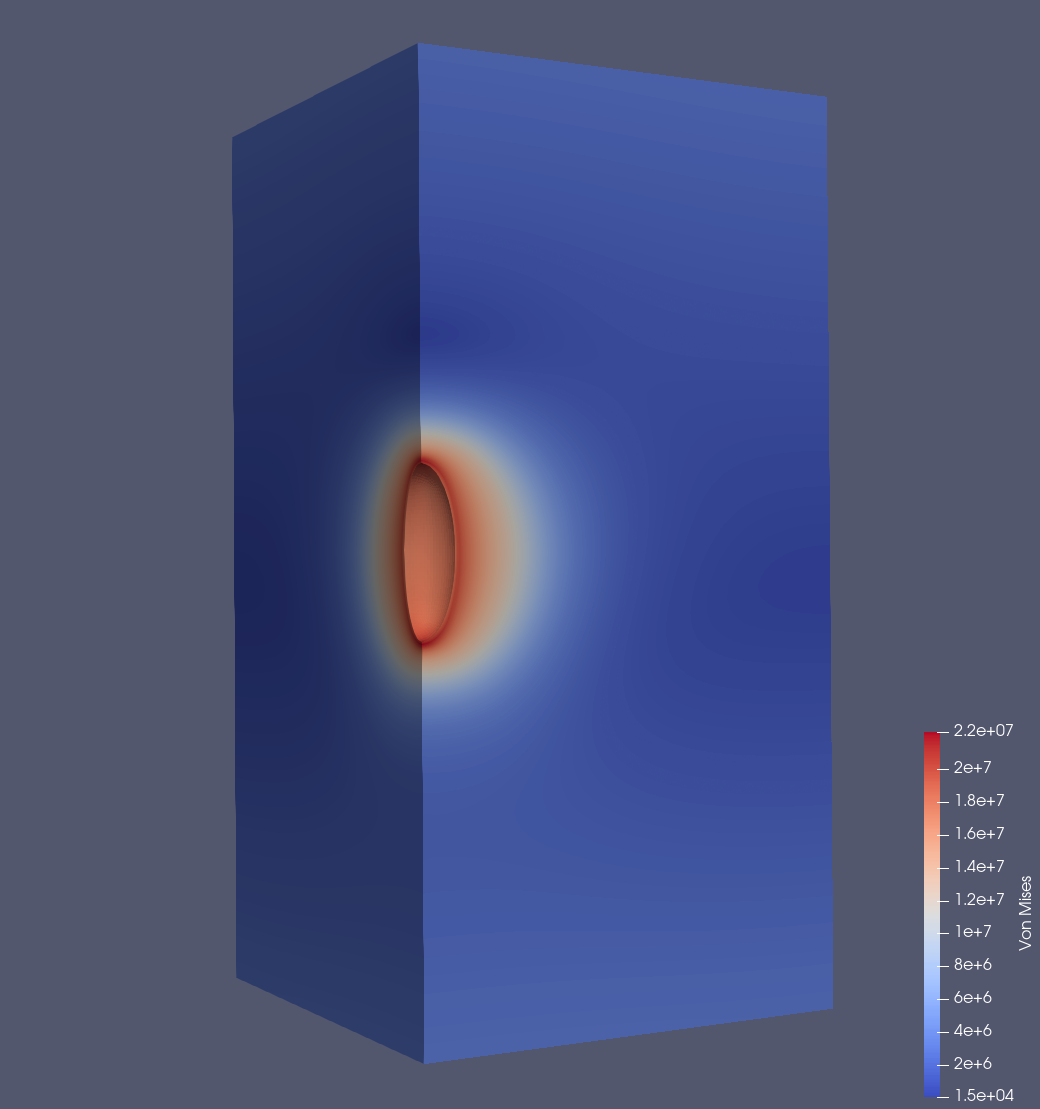
\includegraphics[width=0.95\textwidth]{img/chap5/1dMises应力云图.png}
        \end{minipage}
        \label{fig:Mises1d}
    }
    \subfigure[运行\SI{7}{d}围岩应力云图]
    {
        \begin{minipage}{7cm}
            \centering
            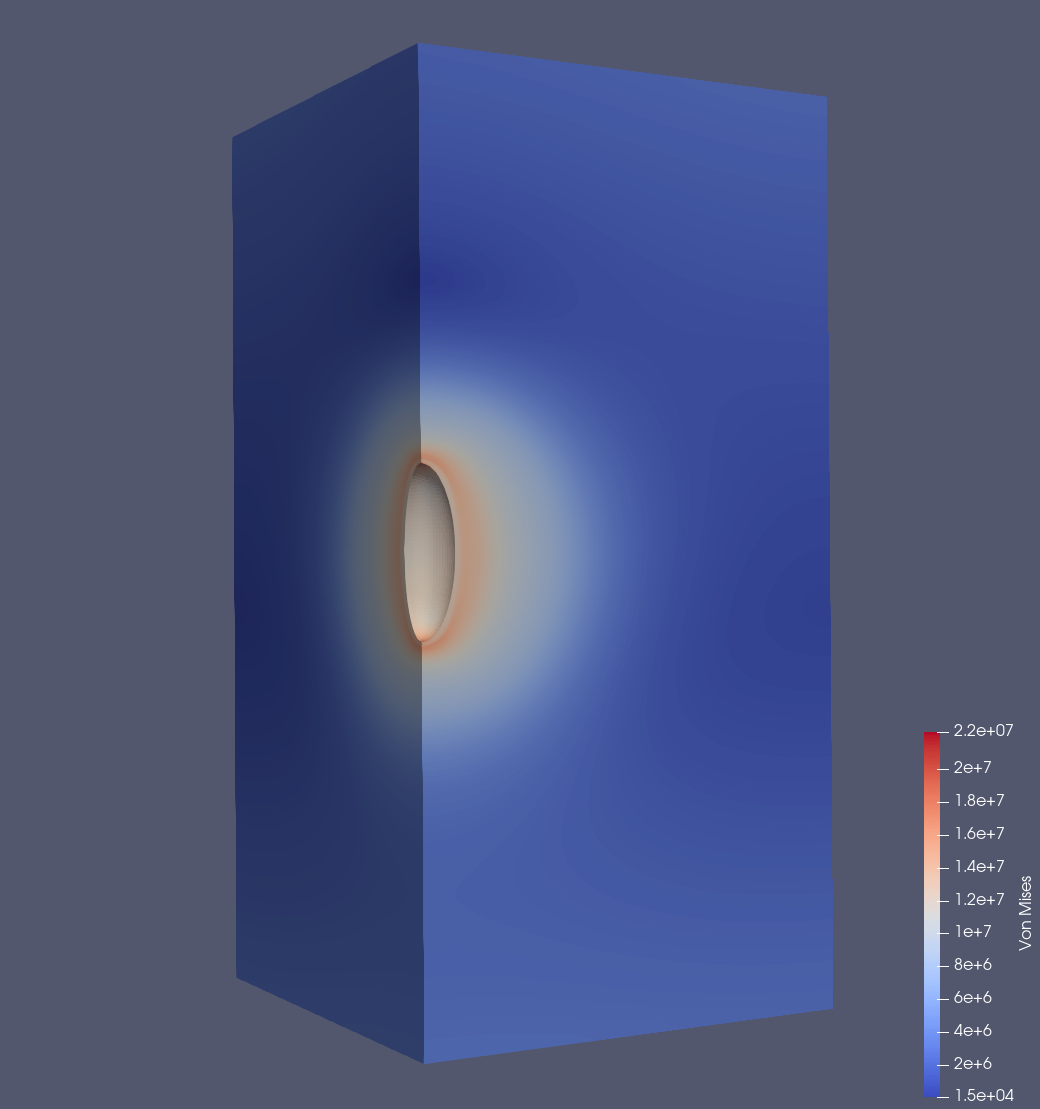
\includegraphics[width=0.95\textwidth]{img/chap5/7dMises应力云图.png}
        \end{minipage}
        \label{fig:Mises7d}
    }
    \caption{运行\SI{1}{d}、\SI{7}{d}后围岩Von Mises应力云图(单位:Pa)}
    \label{fig:Mises}
\end{figure}

\begin{figure}[ht!]
    \centering

    \subfigure[运行\SI{1}{d}围岩温度云图]
    {
        \begin{minipage}{7cm}
            \centering
            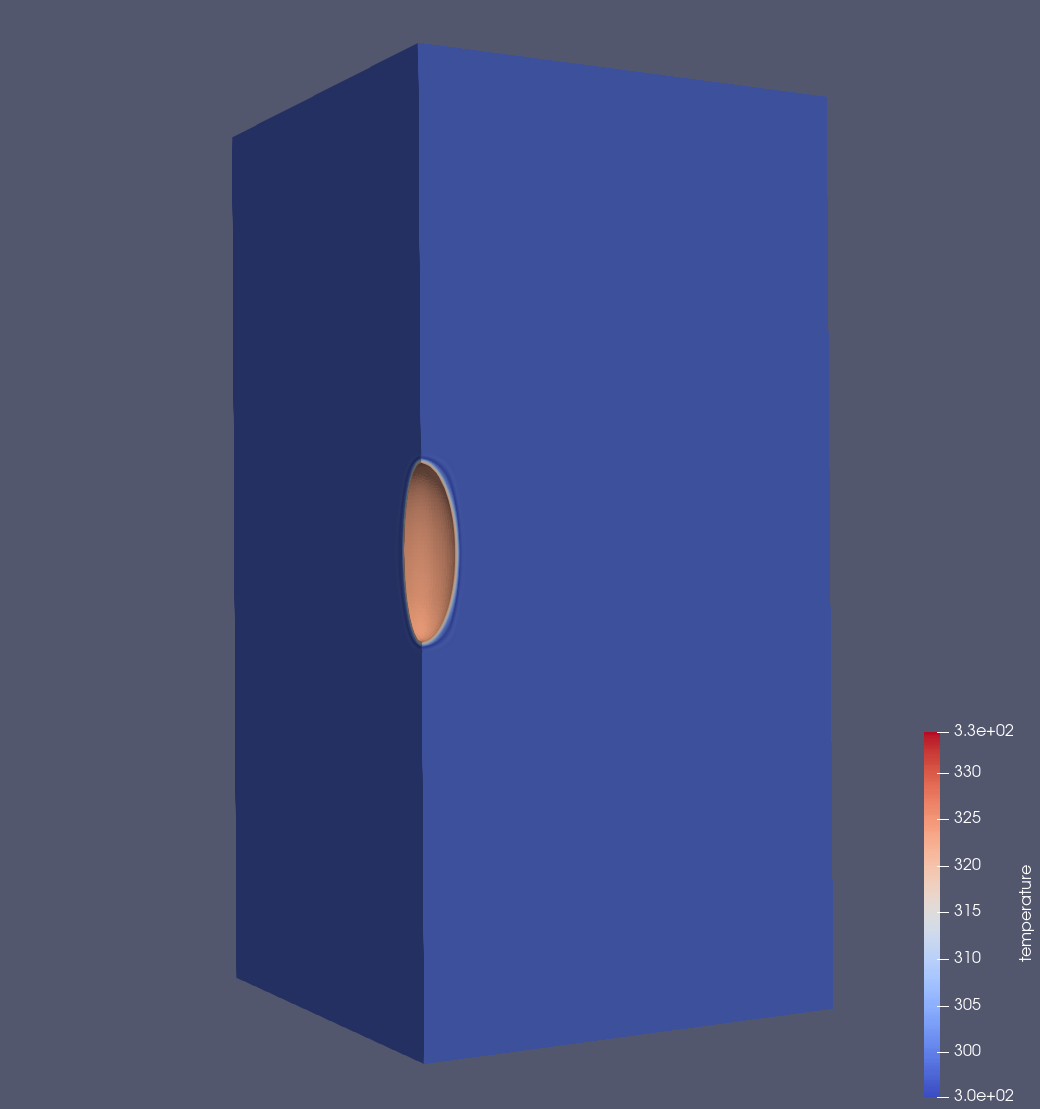
\includegraphics[width=0.95\textwidth]{img/chap5/1d温度云图.png}
        \end{minipage}
        \label{fig:temperature1d}
    }
    \subfigure[运行\SI{7}{d}围岩温度云图]
    {
        \begin{minipage}{7cm}
            \centering
            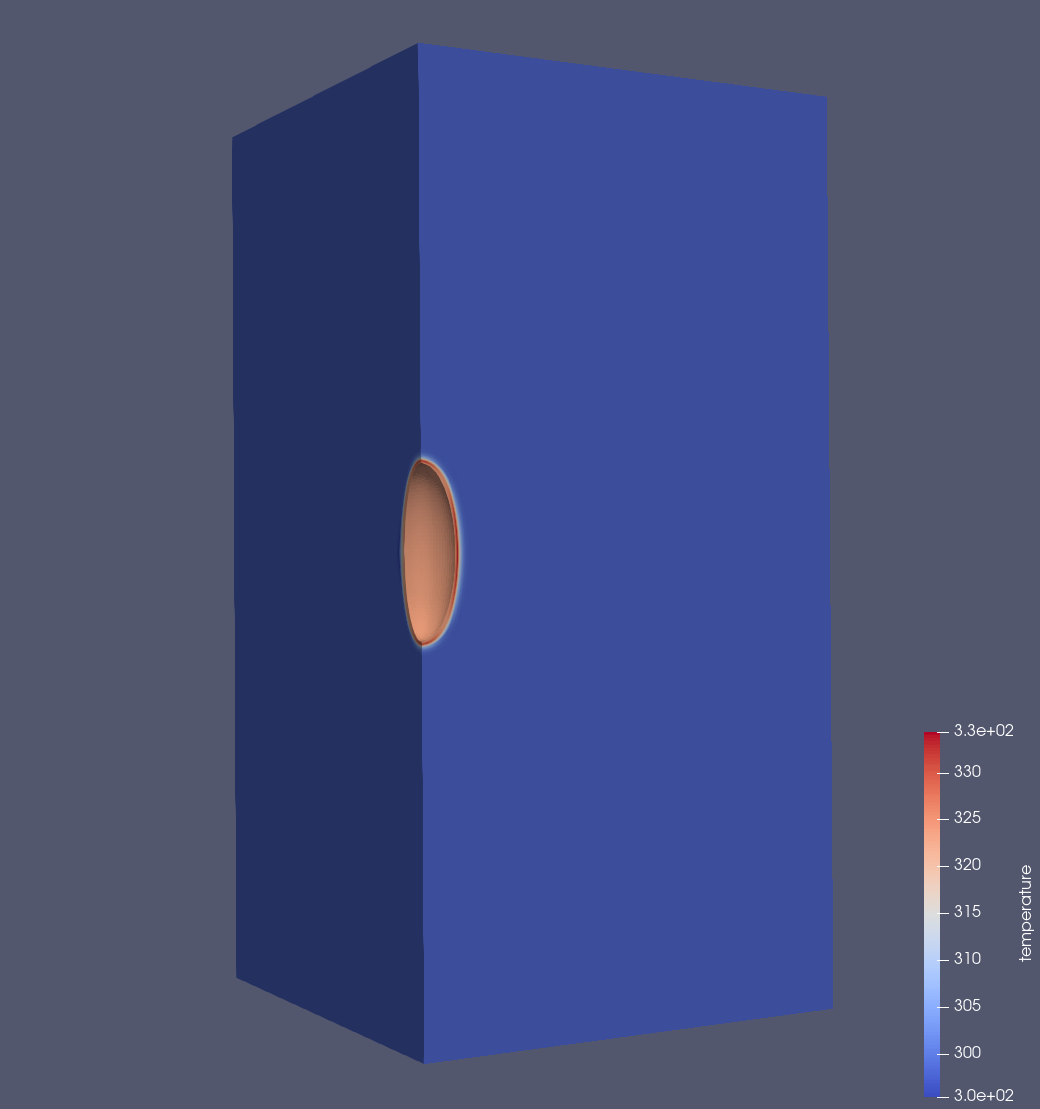
\includegraphics[width=0.95\textwidth]{img/chap5/7d温度云图.png}
        \end{minipage}
        \label{fig:temperature7d}
    }
    \caption{\SI{1}{d}、\SI{7}{d}围岩温度云图(单位:K)}
    \label{fig:temperature}
\end{figure}

\subsubsection{温度}
围岩温度云图如图~\ref{fig:temperature}所示,图~\ref{fig:temperature1d}为运行\SI{1}{d}后温度云图,图~\ref{fig:temperature7d}为运行\SI{7}{d}后温度云图。围岩初始温度为\SI{298}{K},储库运行时气体温度最高为\SI{378}{K},最低为\SI{323}{K},由于温差气体与围岩会发生热交换,导致围岩温度上升。由图可以看出,围岩温度随着与溶腔的距离发生均匀变化。且温度影响范围并不大,运行\SI{1}{d}后,温度影响范围在在\SI{1.5}{m}以内;运行\SI{7}{d}后,温度影响范围在\SI{2.5}{m}以内,可见图~\ref{fig:temperaturefanwei}。

\begin{figure}[ht!]
    \centering
    \subfigure[运行\SI{1}{d}围岩温度变化范围]
    {
        \begin{minipage}{7cm}
            \centering
            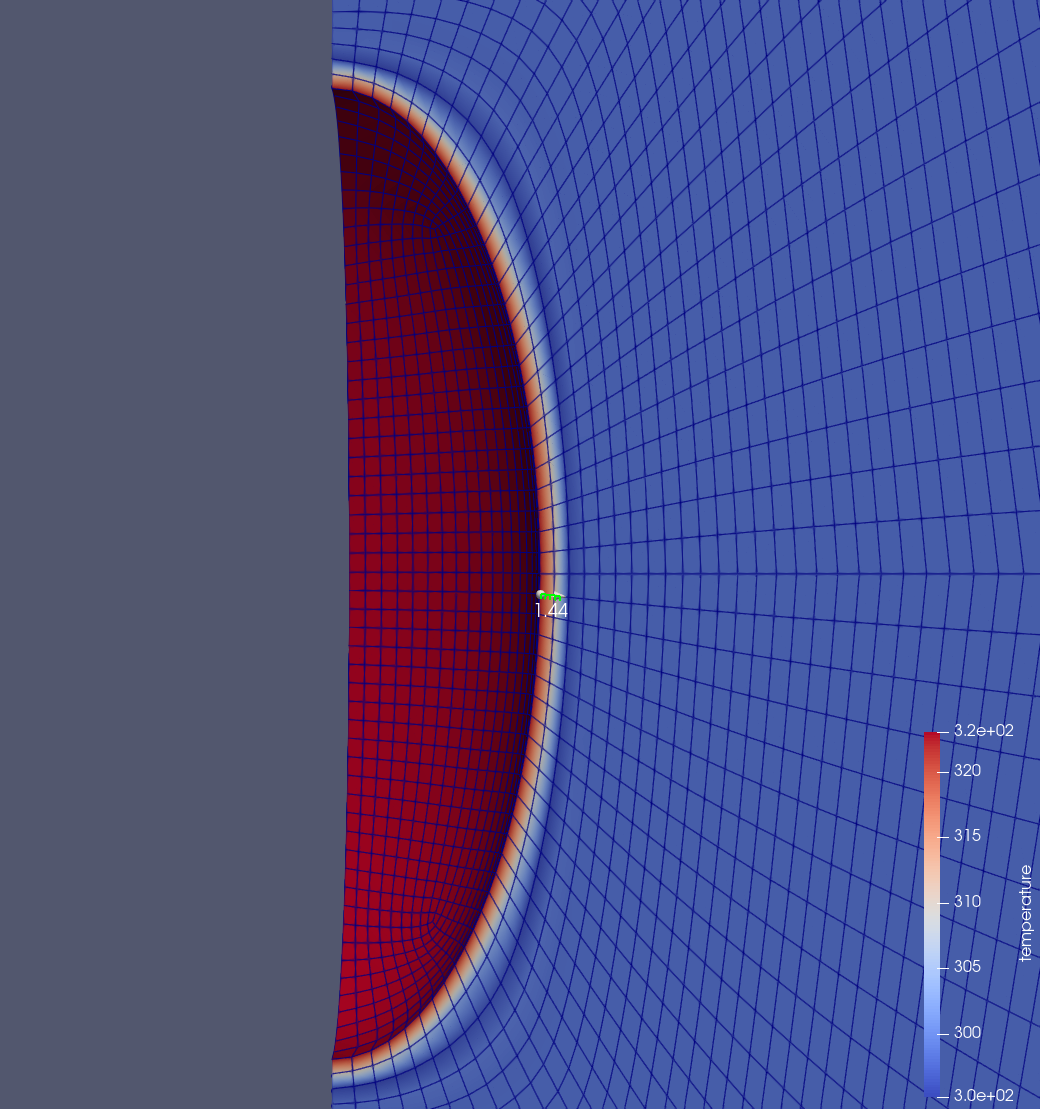
\includegraphics[width=0.95\textwidth]{img/chap5/1d温度影响范围.png}
        \end{minipage}
       
    }
    \subfigure[运行\SI{7}{d}围岩温度影响范围]
    {
        \begin{minipage}{7cm}
            \centering
            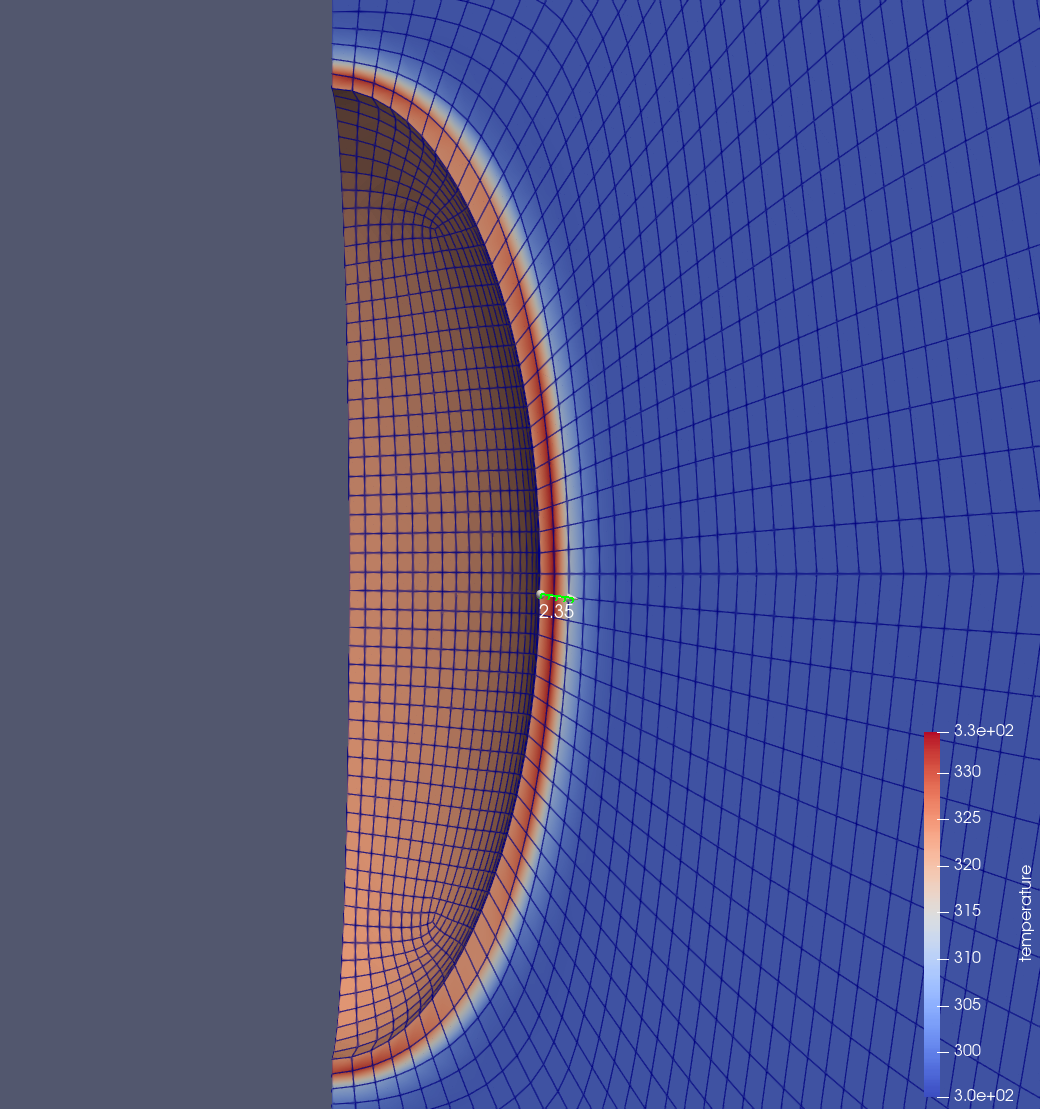
\includegraphics[width=0.95\textwidth]{img/chap5/7d温度影响范围.png}
        \end{minipage}
       
    }
    \caption{\SI{1}{d}、\SI{7}{d}围岩温度影响范围(单位:K)}
    \label{fig:temperaturefanwei}
\end{figure}

运行\SI{7}{d}结束后,围岩最高温度为\SI{334.29}{K},但在每个周期运行约\SI{0.3}{d}后温度达到最大值,为\SI{377.35}{K}。由于腔体内气体温度呈周期性变化,因此围岩的温度在每个周期的前\SI{0.3}{d}随着气体温度迅速升高,在\SI{0.3}{d}达到温度最大值,随后溶腔附近的高温围岩向低温围岩传热,温度下降,并不会造成热量的大量累积。

\begin{figure}[ht!]
    \centering
    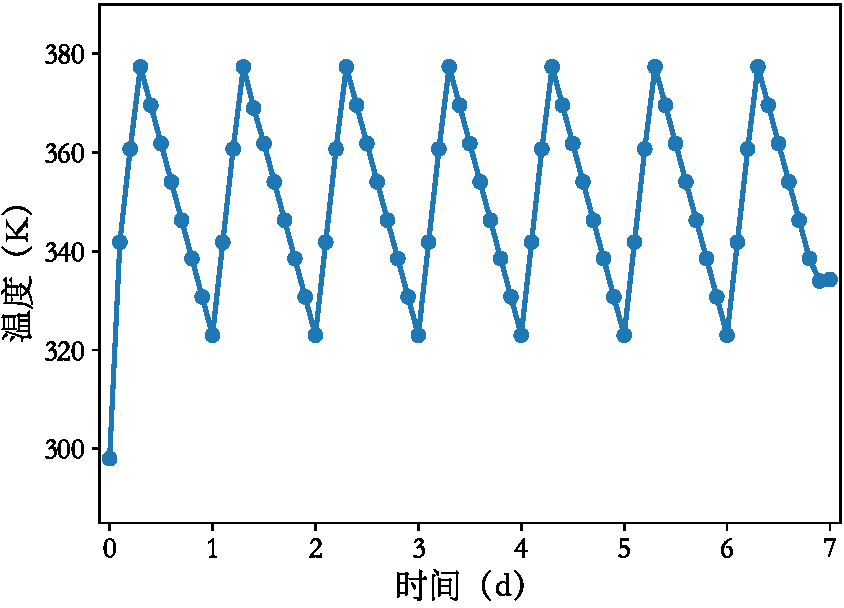
\includegraphics[width=0.55\textwidth]{img/chap5/7d最大温度.pdf}
    \caption{\SI{7}{d}内围岩最大温度与时间变化曲线}
    \label{fig:7d_temperature_t}
\end{figure}

围岩最高温度随时间变化的关系曲线如图所示~\ref{fig:7d_temperature_t}。由该曲线图可以看出,围岩温度在第一个周期内快速上升,自第一个周期以后在\SI{323}{K}-\SI{377.35}{K}之间作周期变化,达到\SI{377.35}{K}后不在上升,而是不断将热量传递至周围低温岩石,扩大温度影响范围。



\section{计算效率分析}
通过对该三维问题的并行计算处理,将原模型划分成多个子模型,借助超级计算机的不同处理器对多个子模型同时求解,可有效提高计算速度和处理能力。但因为非线性边界条件的存在,能够收敛的步长较小,目前计算步长取\SI{0.001}{d},计算模拟\SI{7}{d}运行一共需7000步。利用无锡超算中心商用平台计算,运行完7天共耗时\SI{75}{h},约为\SI{3.2}{d}。因三维问题求解时间过长,不满足计算的高效性原则,在不严重影响计算精度和计算规律,且保持长期循环温度、荷载不变的条件下改为二维计算。

二维计算模型较小,分割的计算单元少,利用超级计算机进行计算并不能有效提高计算效率,因此,尝试利用单一处理器性能力更强的个人计算机进行模拟。二维模型计算过程中,偏应力比三维中的大,非线性程度较高,步长取与三维中相同的\SI{0.001}{d}无法收敛,因此取\SI{0.0001}{d}进行计算。模拟\SI{7}{d}运行一共需70000步,运行完成共耗时\SI{0.12}{h}。当计算总时长为10年,预计需\SI{60.8}{h},即约\SI{2.5}{d}。求解时间大幅缩短,满足计算高效性原则。

综合上述试算结果及计算效率分析,维持原边界条件不变的情况下,将原三维模型转化为二维模型进行模拟试验。二维模型示意图、二维模型网格划分如图~\ref{fig:2dmodel}所示,共3202单元,3325节点。边界条件见。模型参数见第~\ref{section:modelparameters}节中表~\ref{tab:1}-\ref{tab:3}。

\begin{figure}[ht!]
    \centering
    \subfigure[二维模型简图]
    {
        \begin{minipage}{7cm}
            \centering
            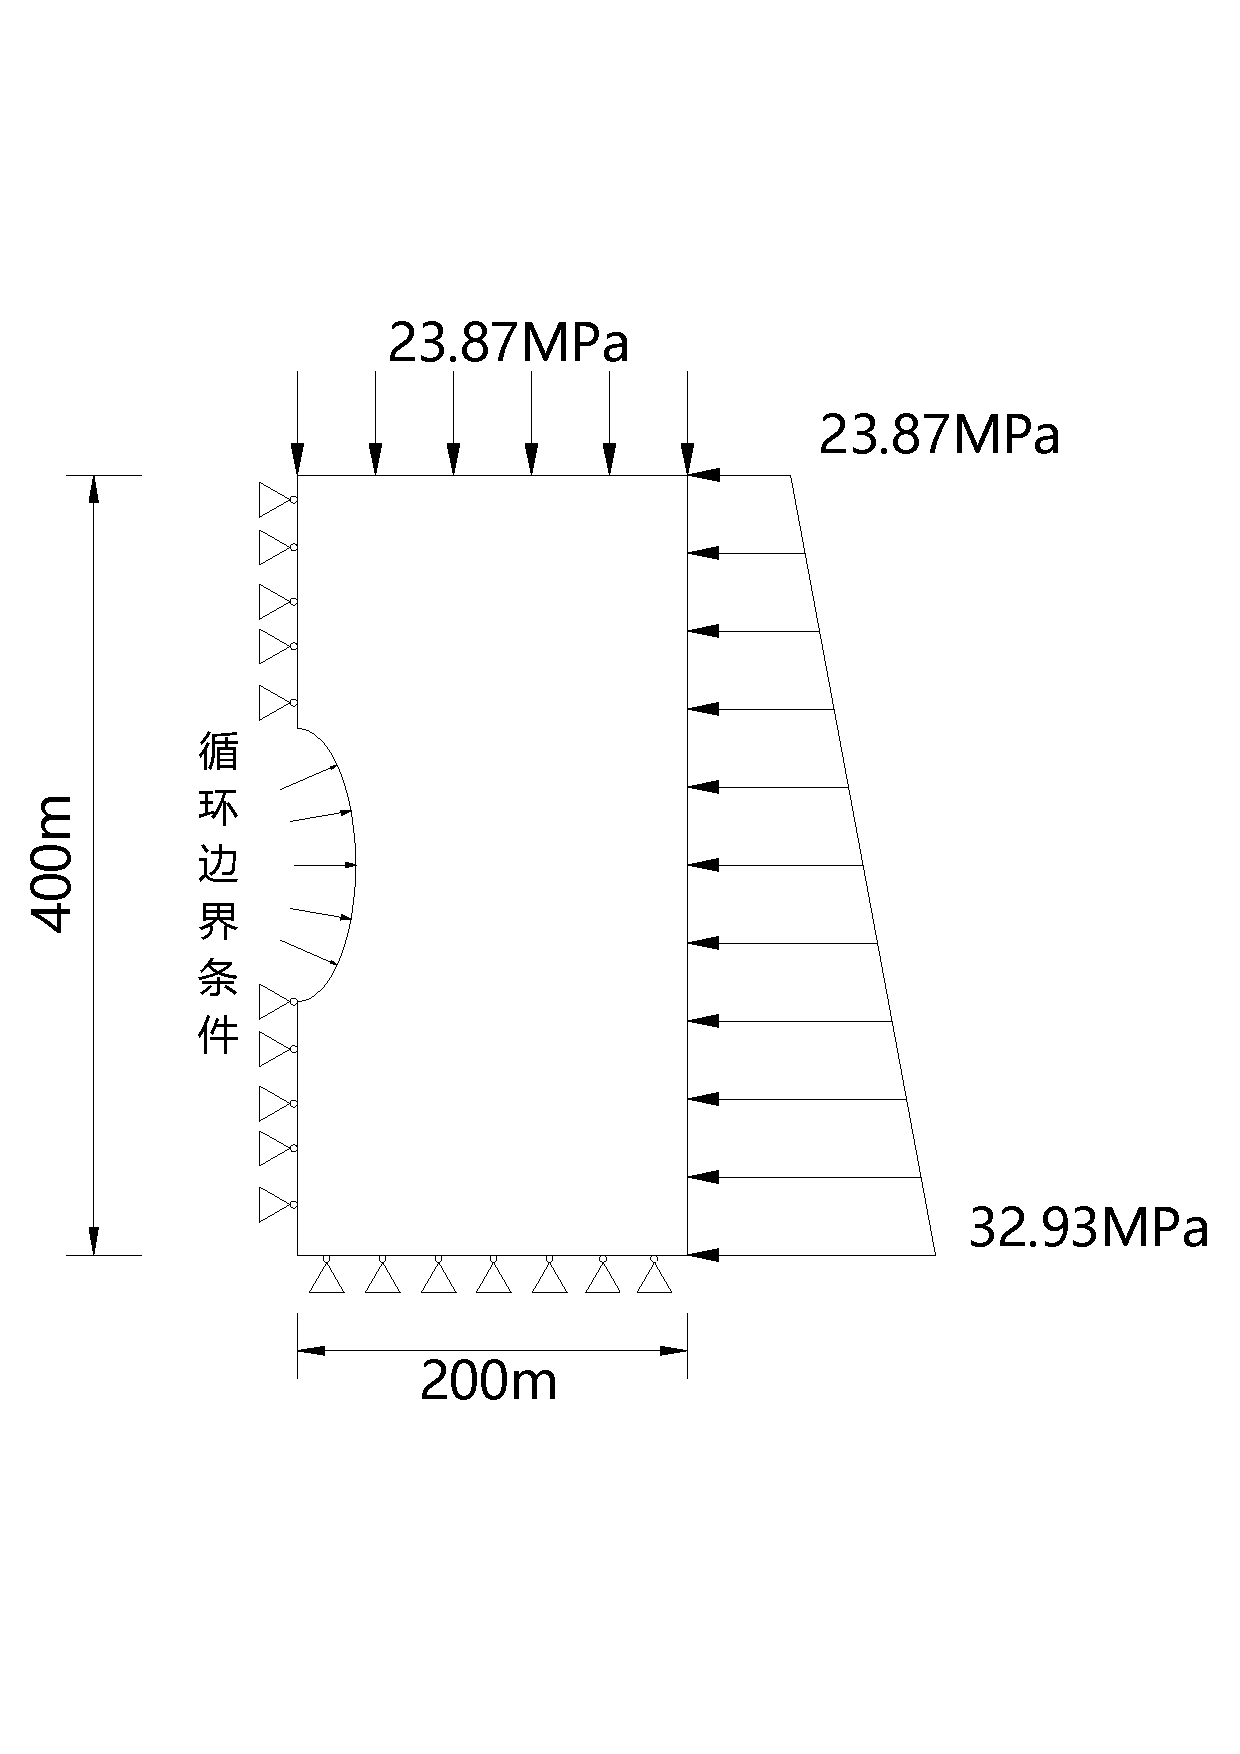
\includegraphics[width=1.0\textwidth]{img/chap5/二维模型.pdf}
        \end{minipage}
    }
    \subfigure[二维模型网格划分图]
    {
        \begin{minipage}{7cm}
            \centering
            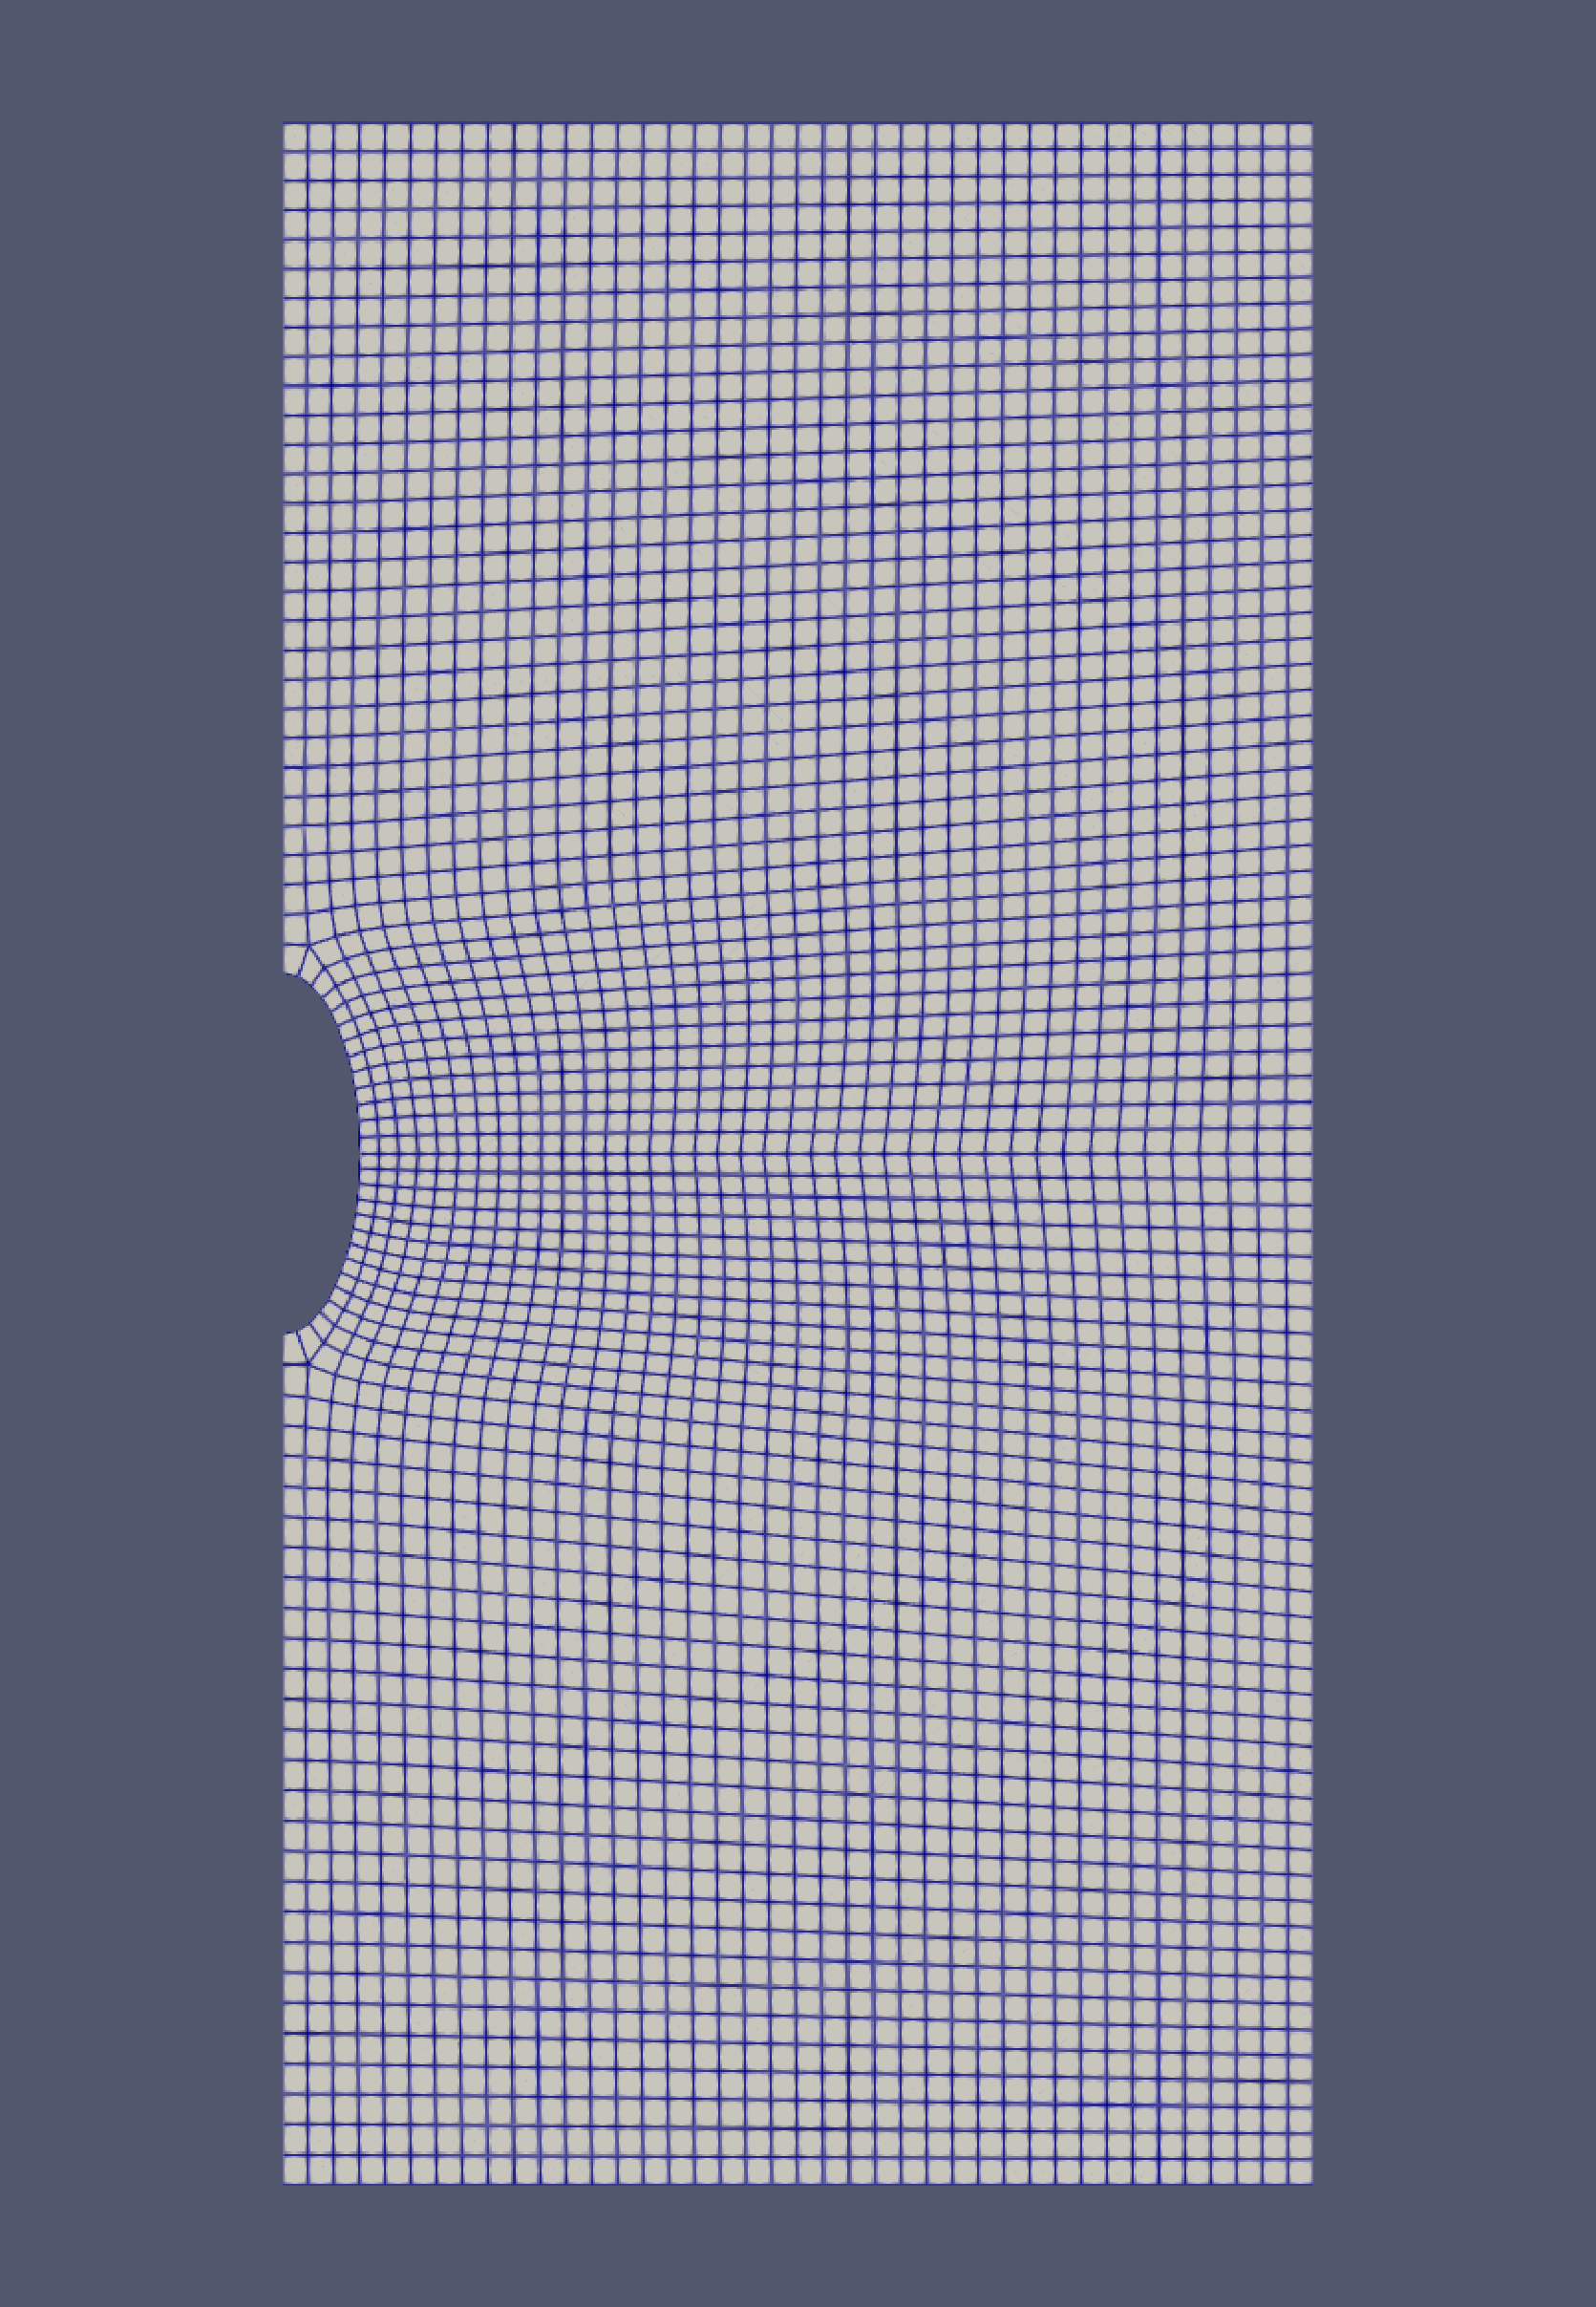
\includegraphics[width=0.95\textwidth]{img/chap5/二维网格.pdf}
        \end{minipage}
    }
    \caption{二维模型简图及网格图}
   %\todoiZN{左边的图的白边可以裁一下。}
    \label{fig:2dmodel}
\end{figure}

\section{新能源储库和传统能源储备库计算结果对比分析}

\subsection{位移分析}

上述不同工况下,储库运行十年后,位移云图如图~\ref{fig:4weiyi}所示。从云图中可以看出,腔体顶部下沉,底部鼓起,腰部向内收缩,且主要集中于腰部。周围岩石因受到的地应力的值大于腔体内气体压力,而产生向内收缩的位移。

\begin{figure}[ht!]
    \centering
    \subfigure[工况一运行\SI{10}{a}后位移云图]
    {
        \begin{minipage}{6.2cm}
            \centering
            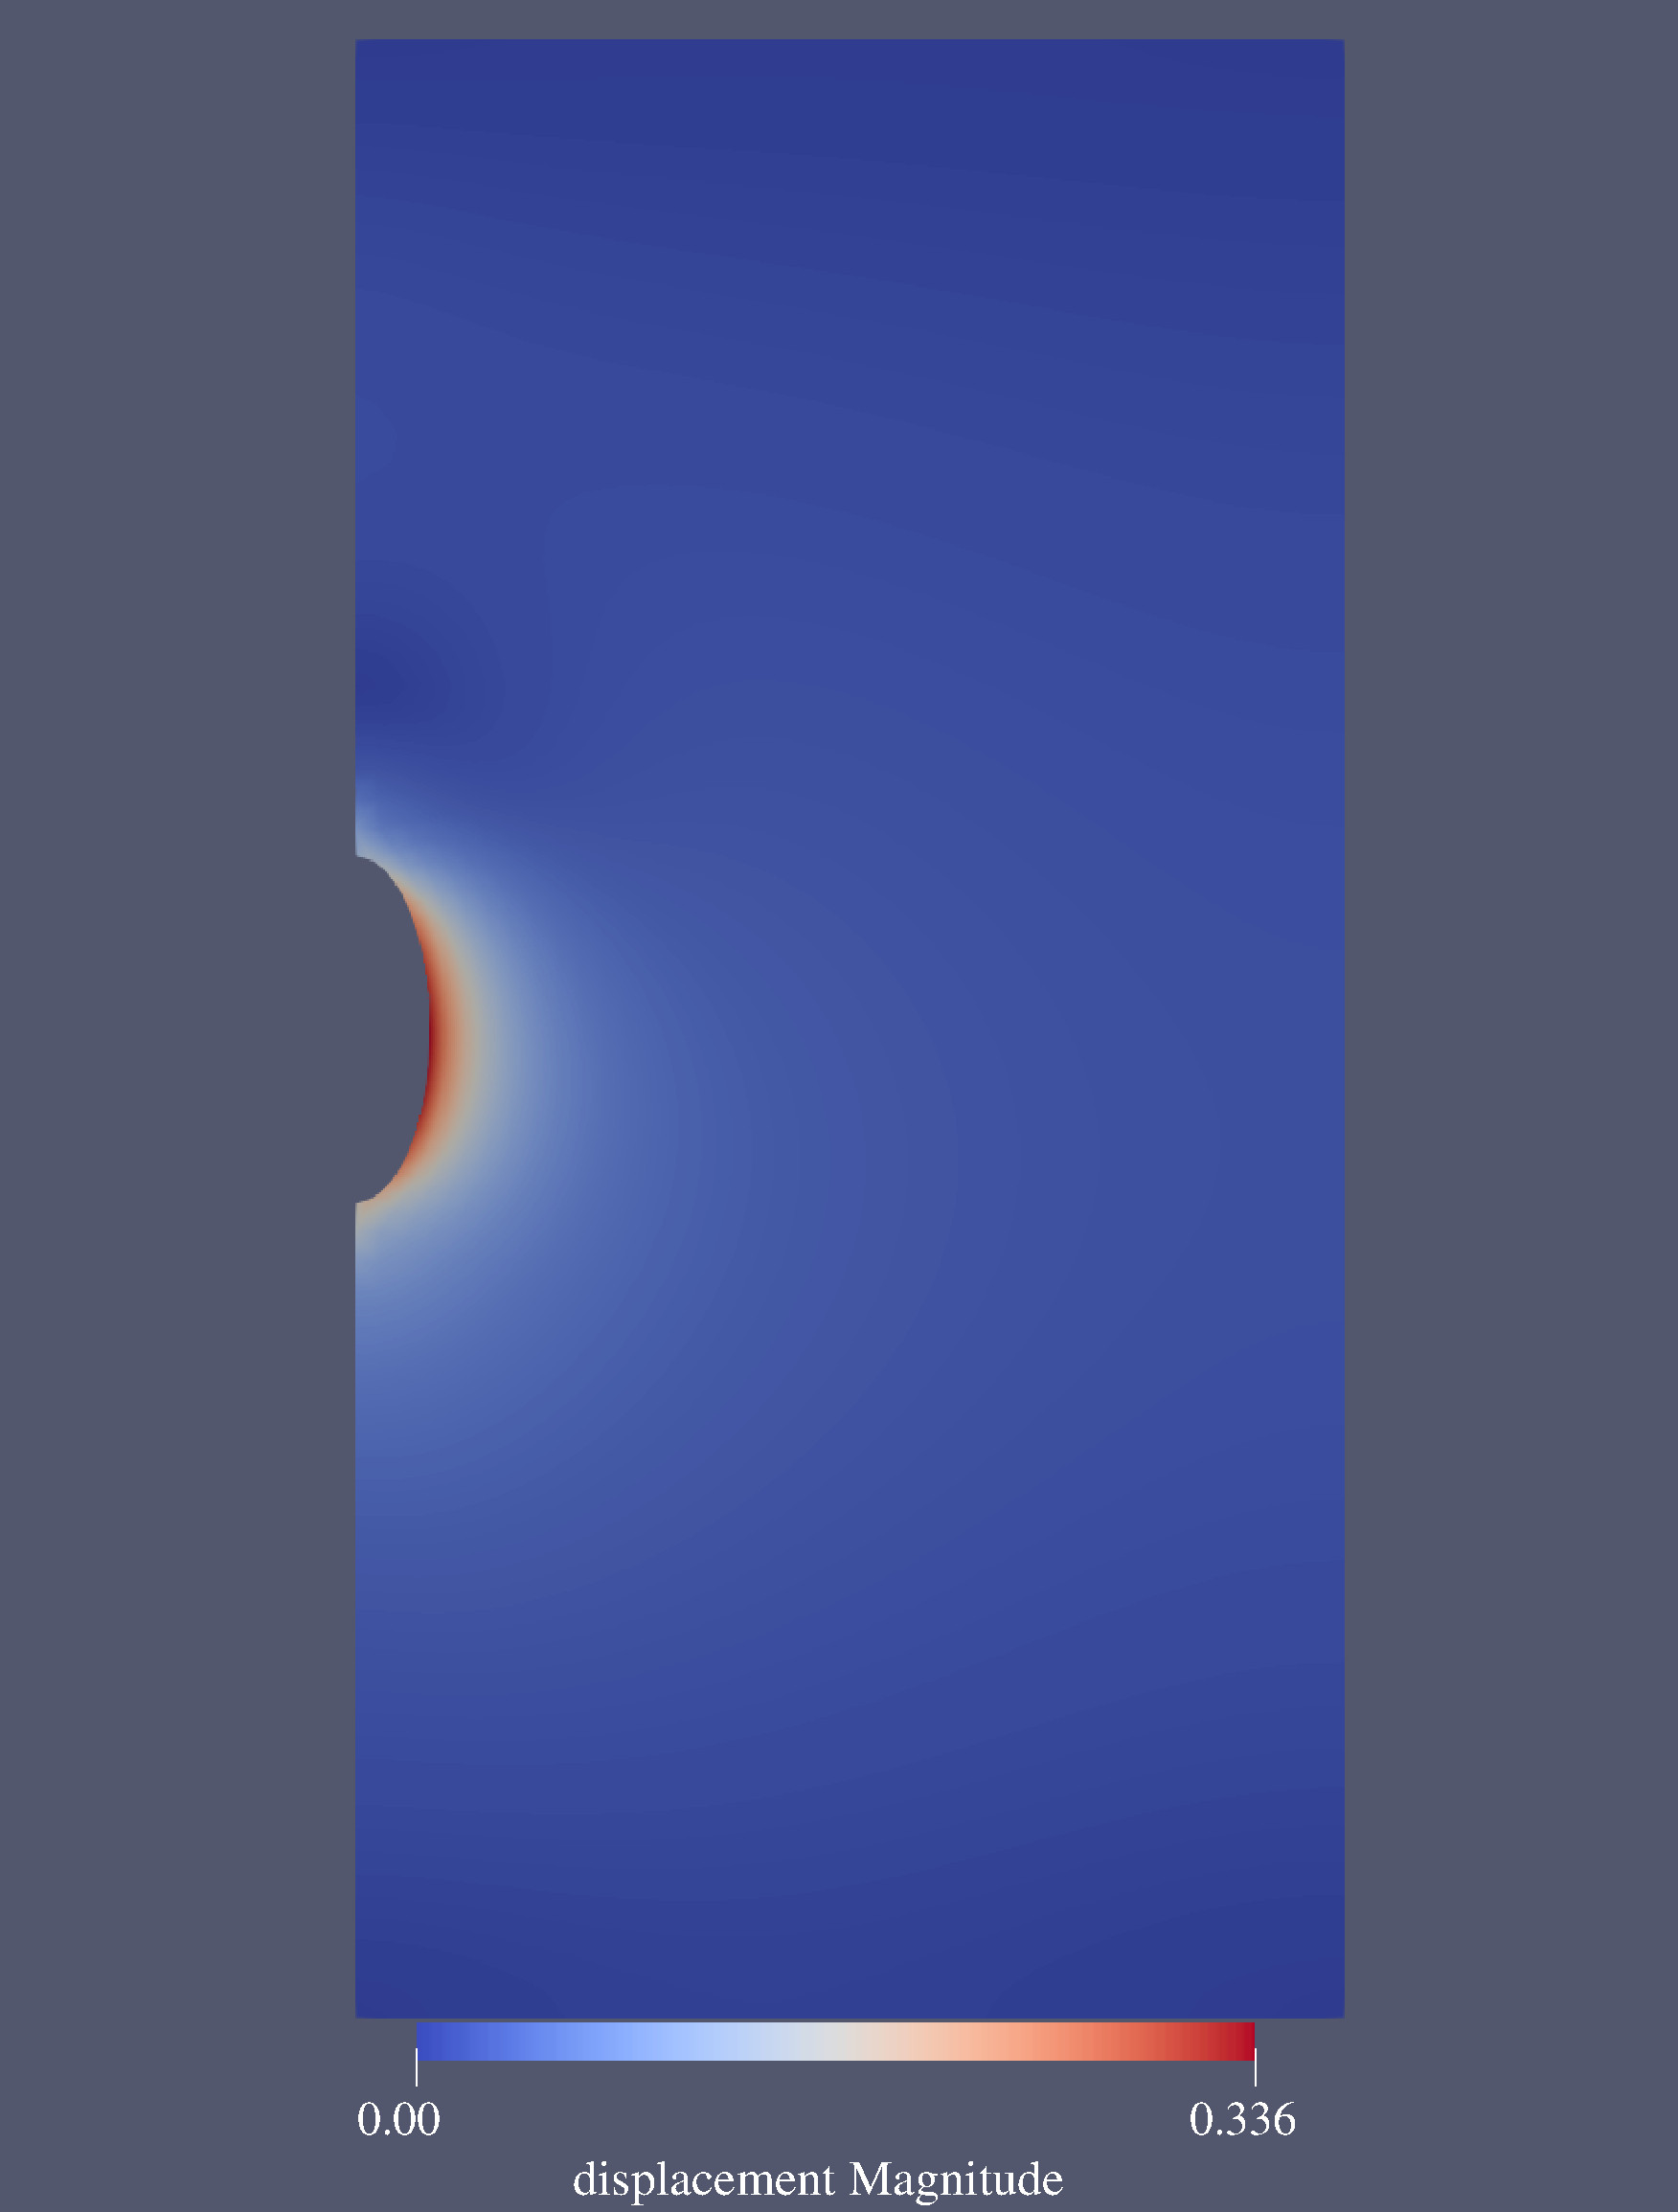
\includegraphics[width=0.95\textwidth]{img/chap5/位移/工况一位移云图.pdf}
        \end{minipage}
    }
    \subfigure[工况二运行\SI{10}{a}后位移云图]
    {
        \begin{minipage}{6.2cm}
            \centering
            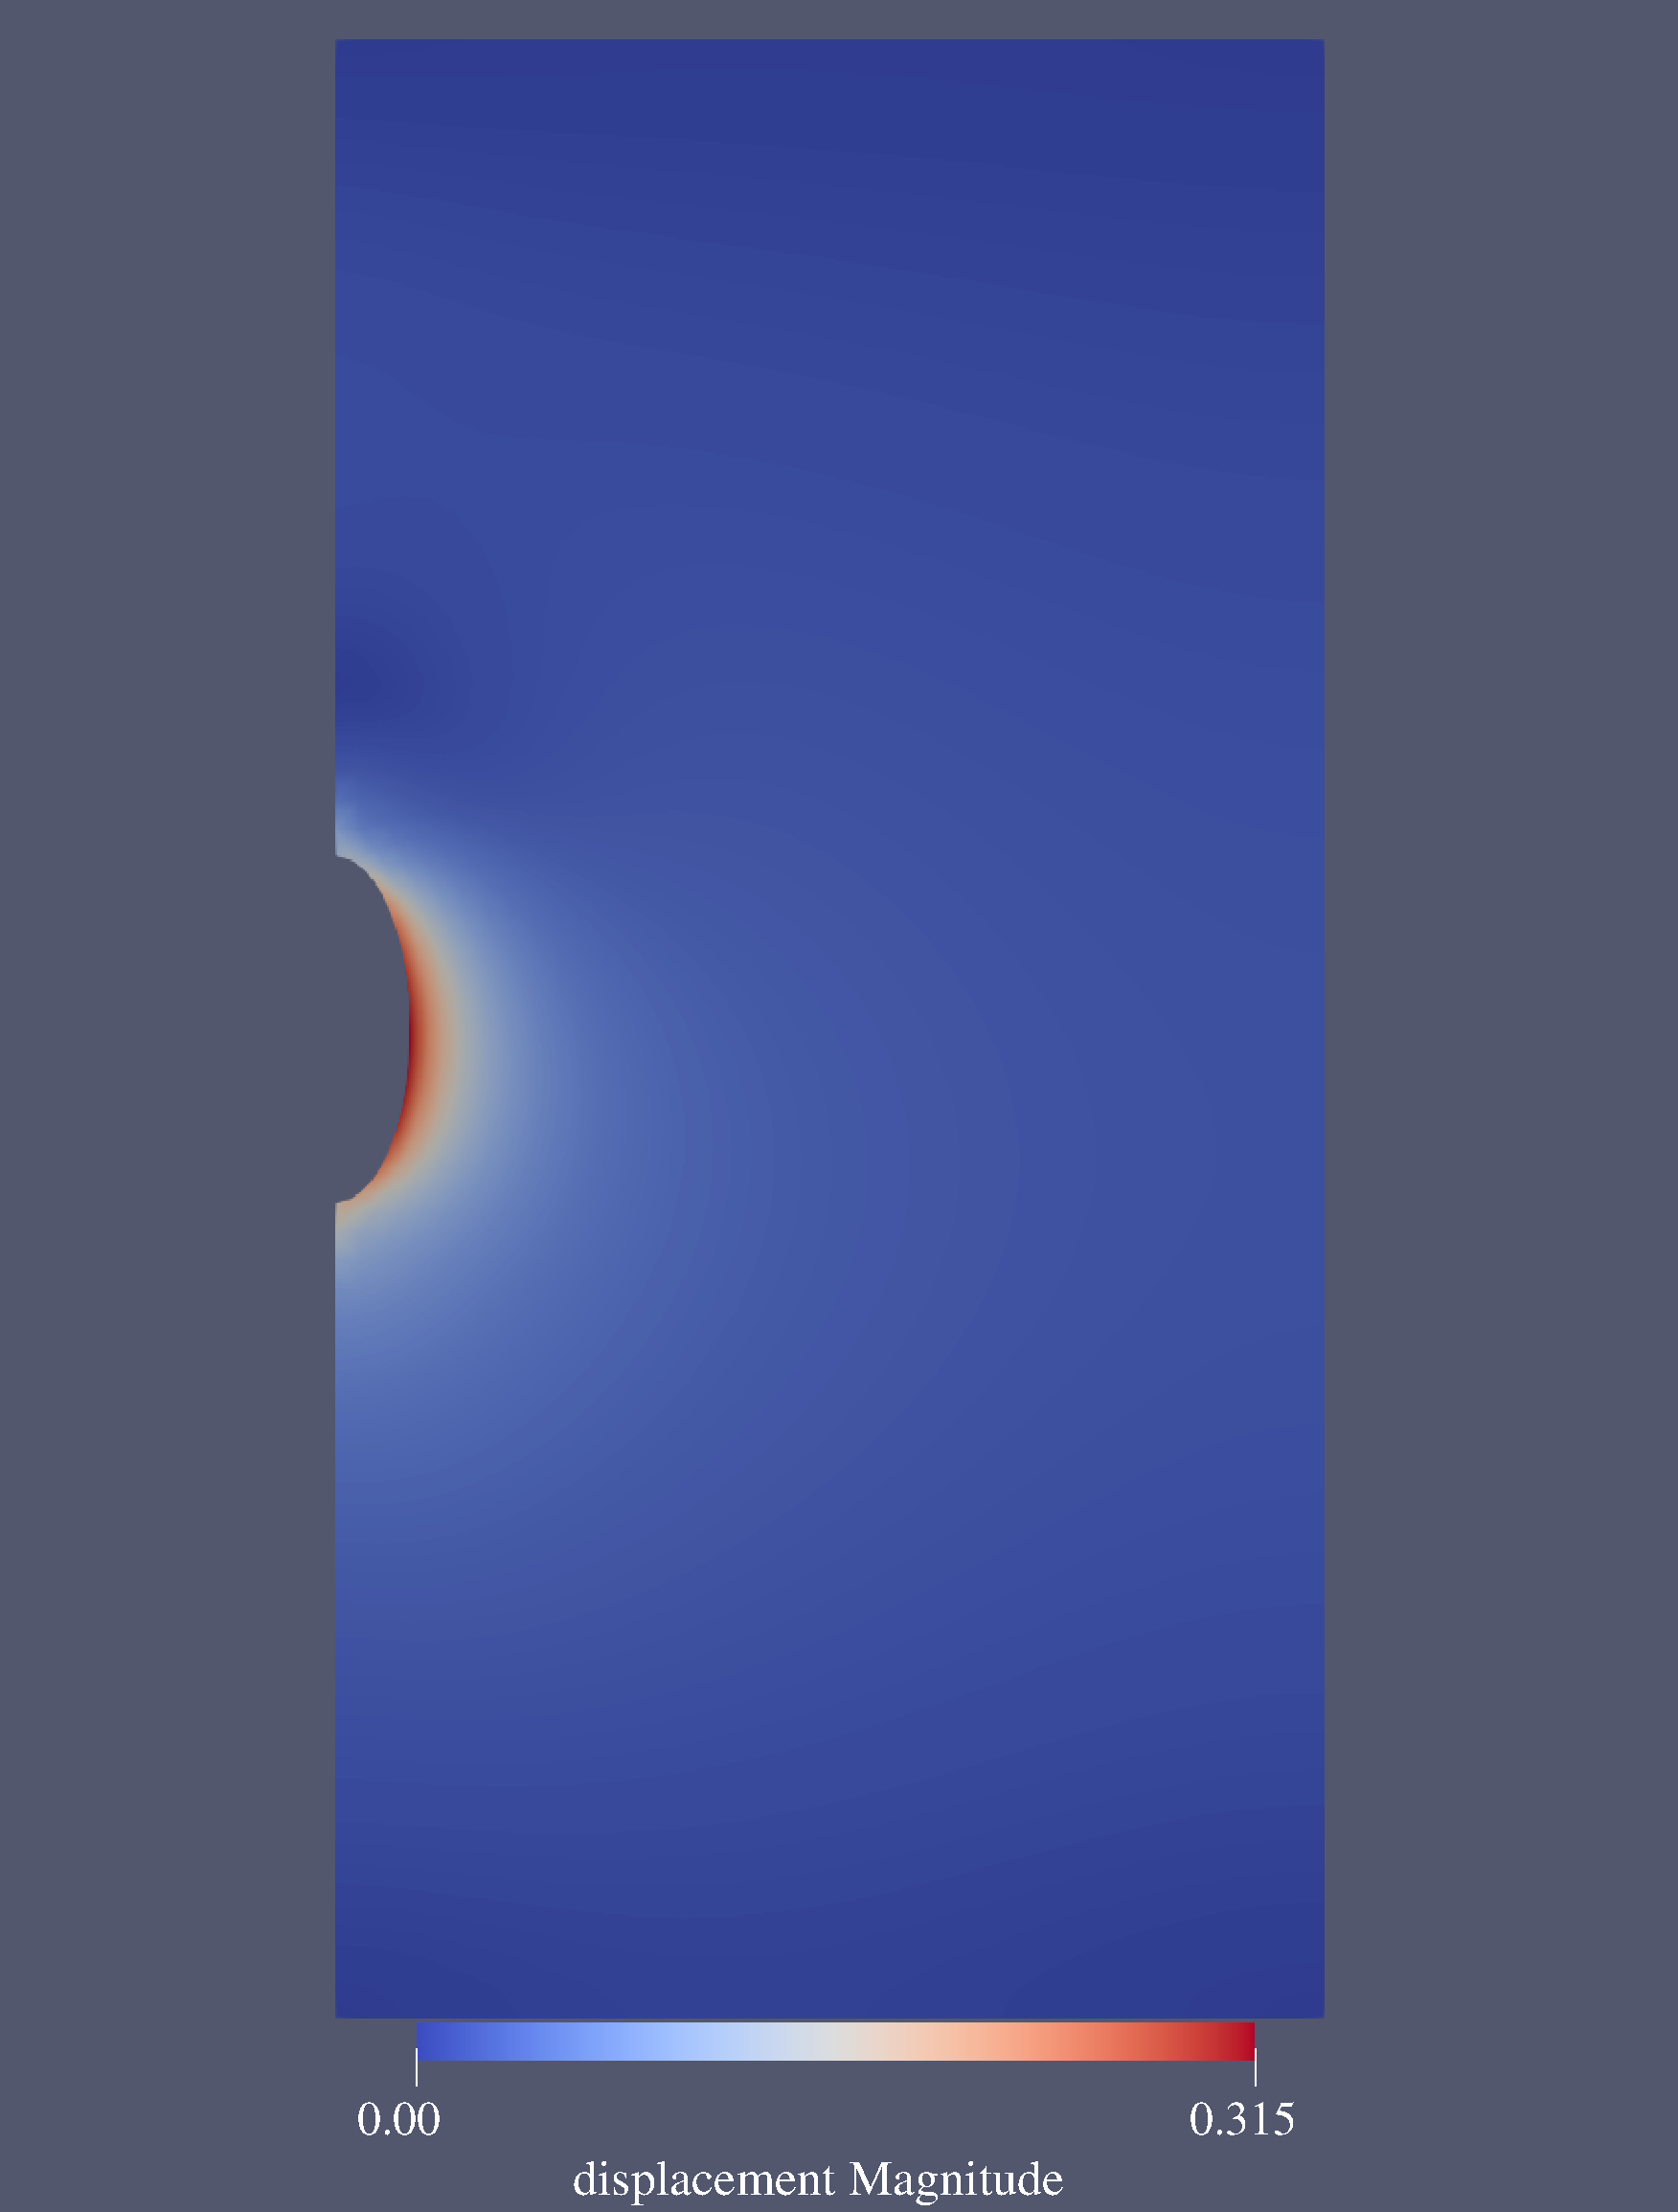
\includegraphics[width=0.95\textwidth]{img/chap5/位移/工况二位移云图.pdf}
        \end{minipage}
    }
    \subfigure[工况三运行\SI{10}{a}后位移云图]
    {
        \begin{minipage}{6.2cm}
            \centering
            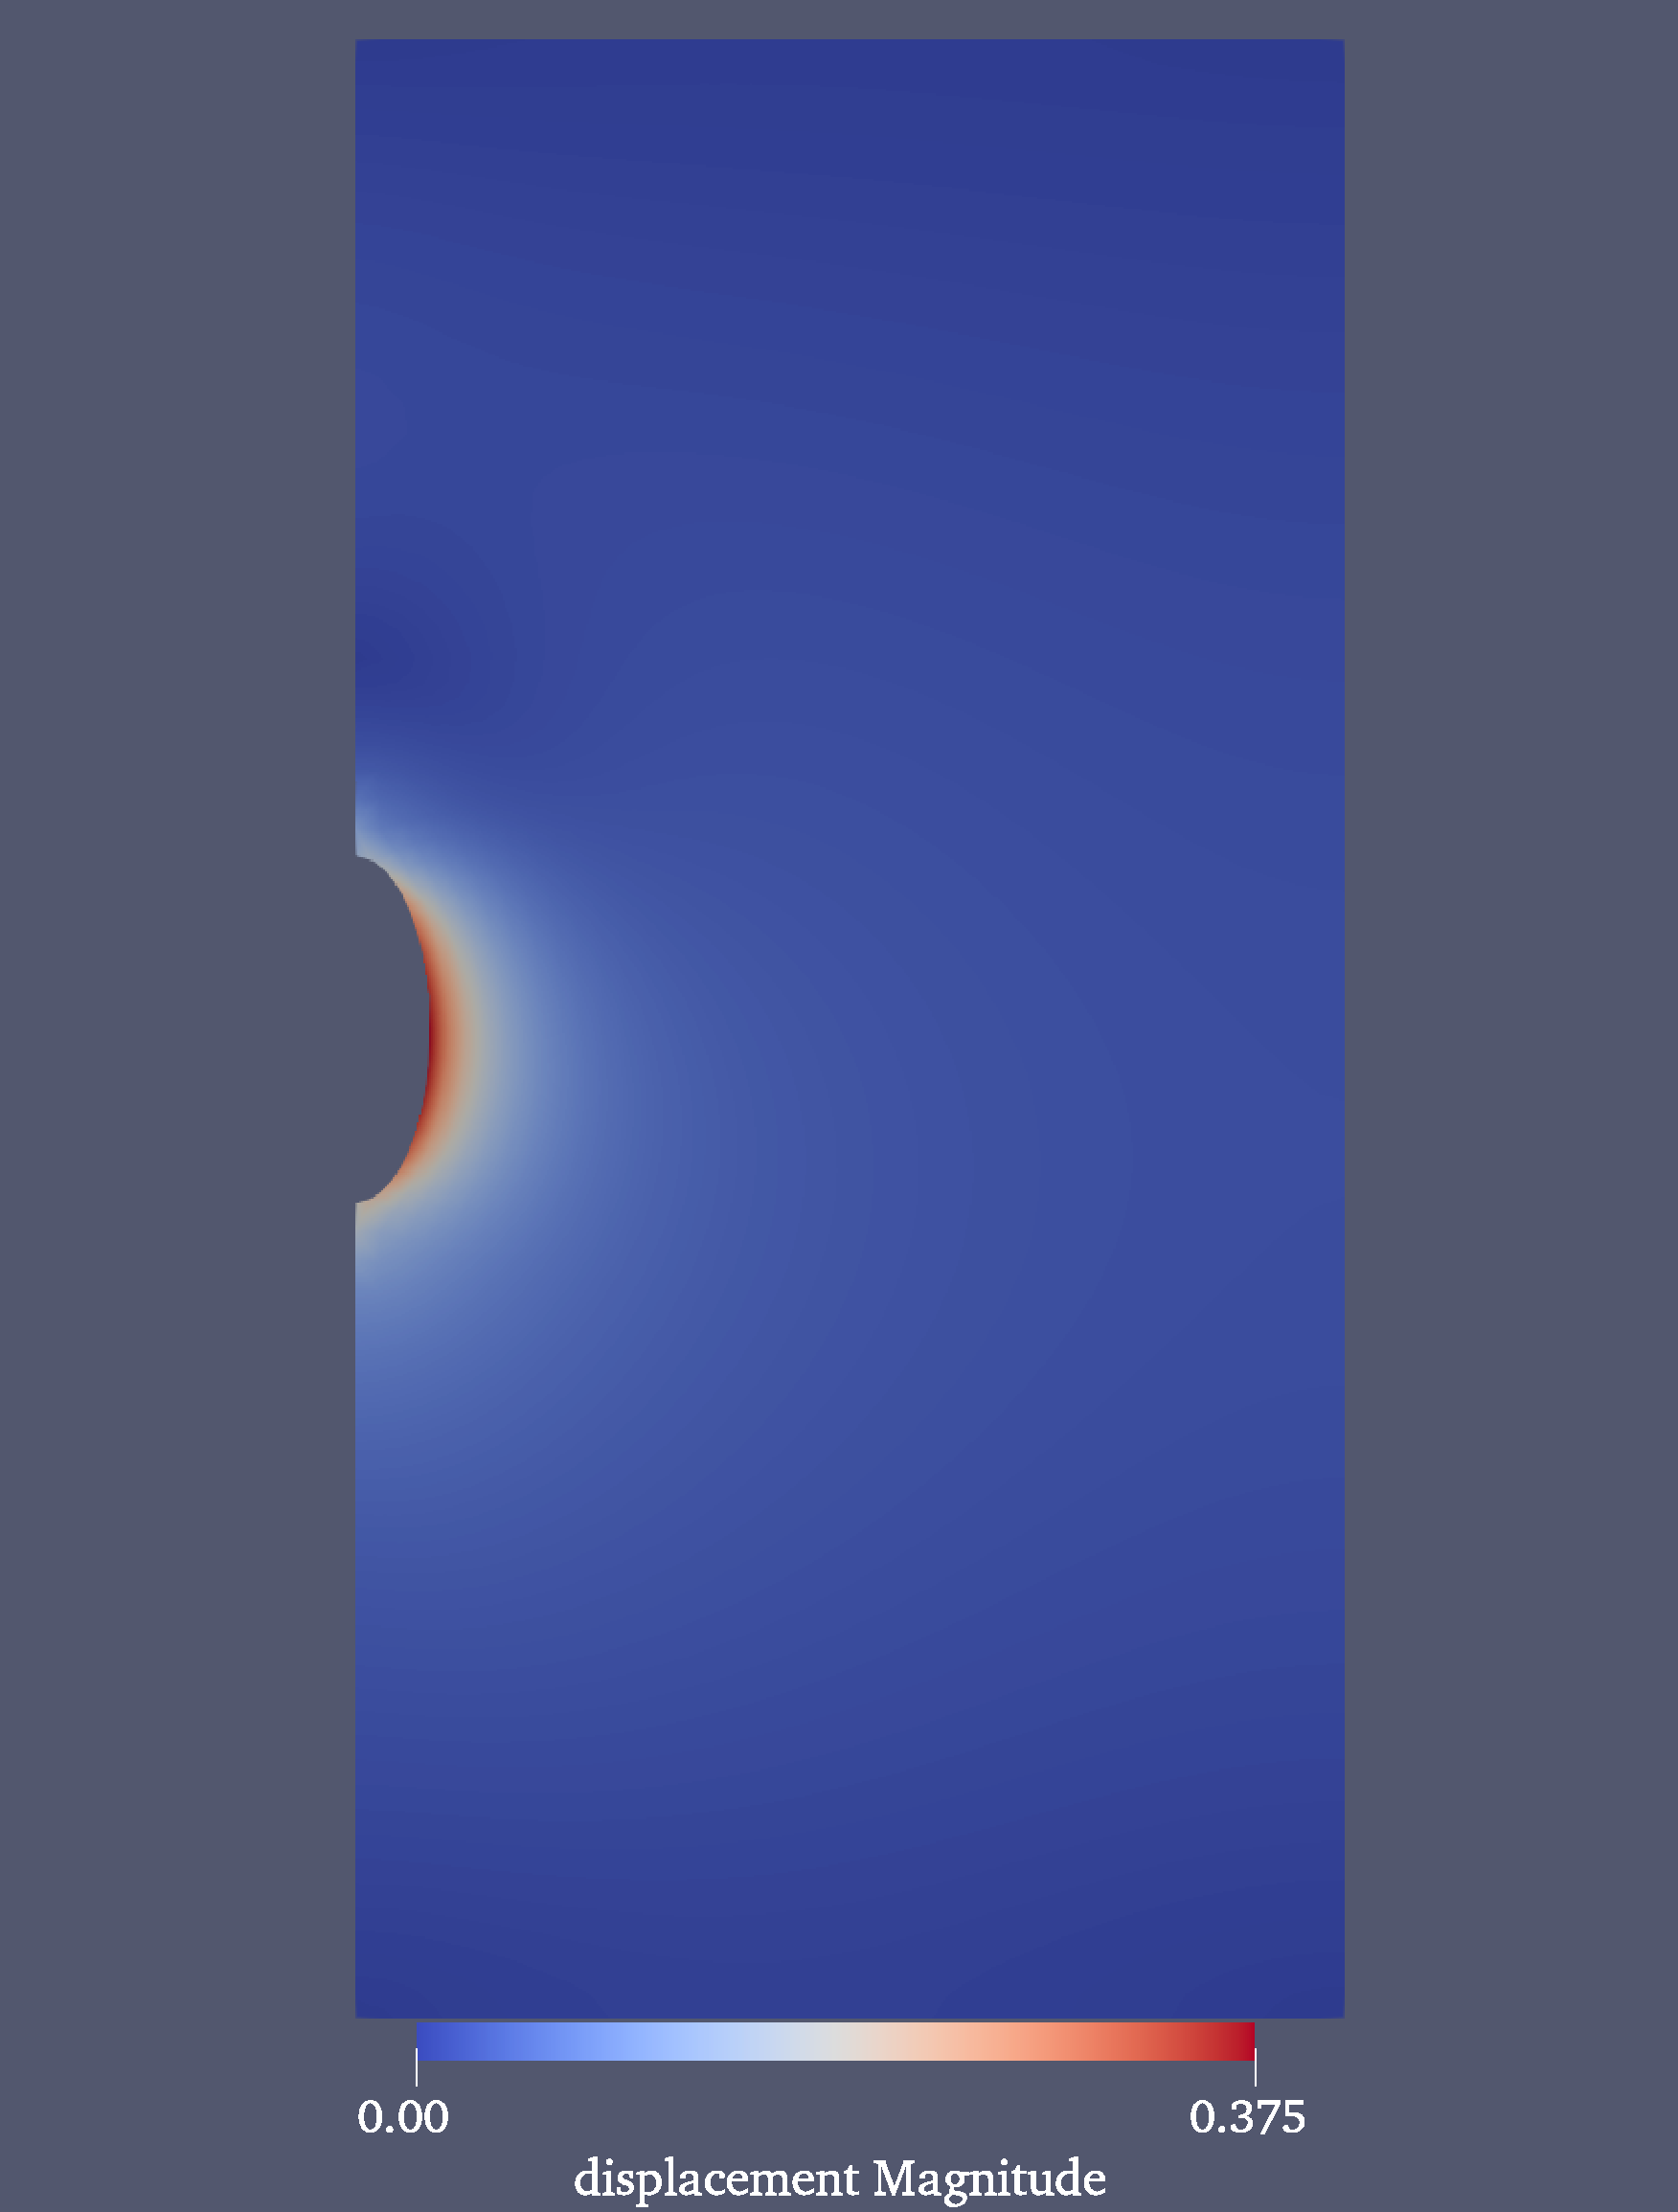
\includegraphics[width=0.95\textwidth]{img/chap5/位移/工况三位移云图.pdf}
        \end{minipage}
    }
    \subfigure[工况四运行\SI{10}{a}后位移云图]
    {
        \begin{minipage}{6.2cm}
            \centering
            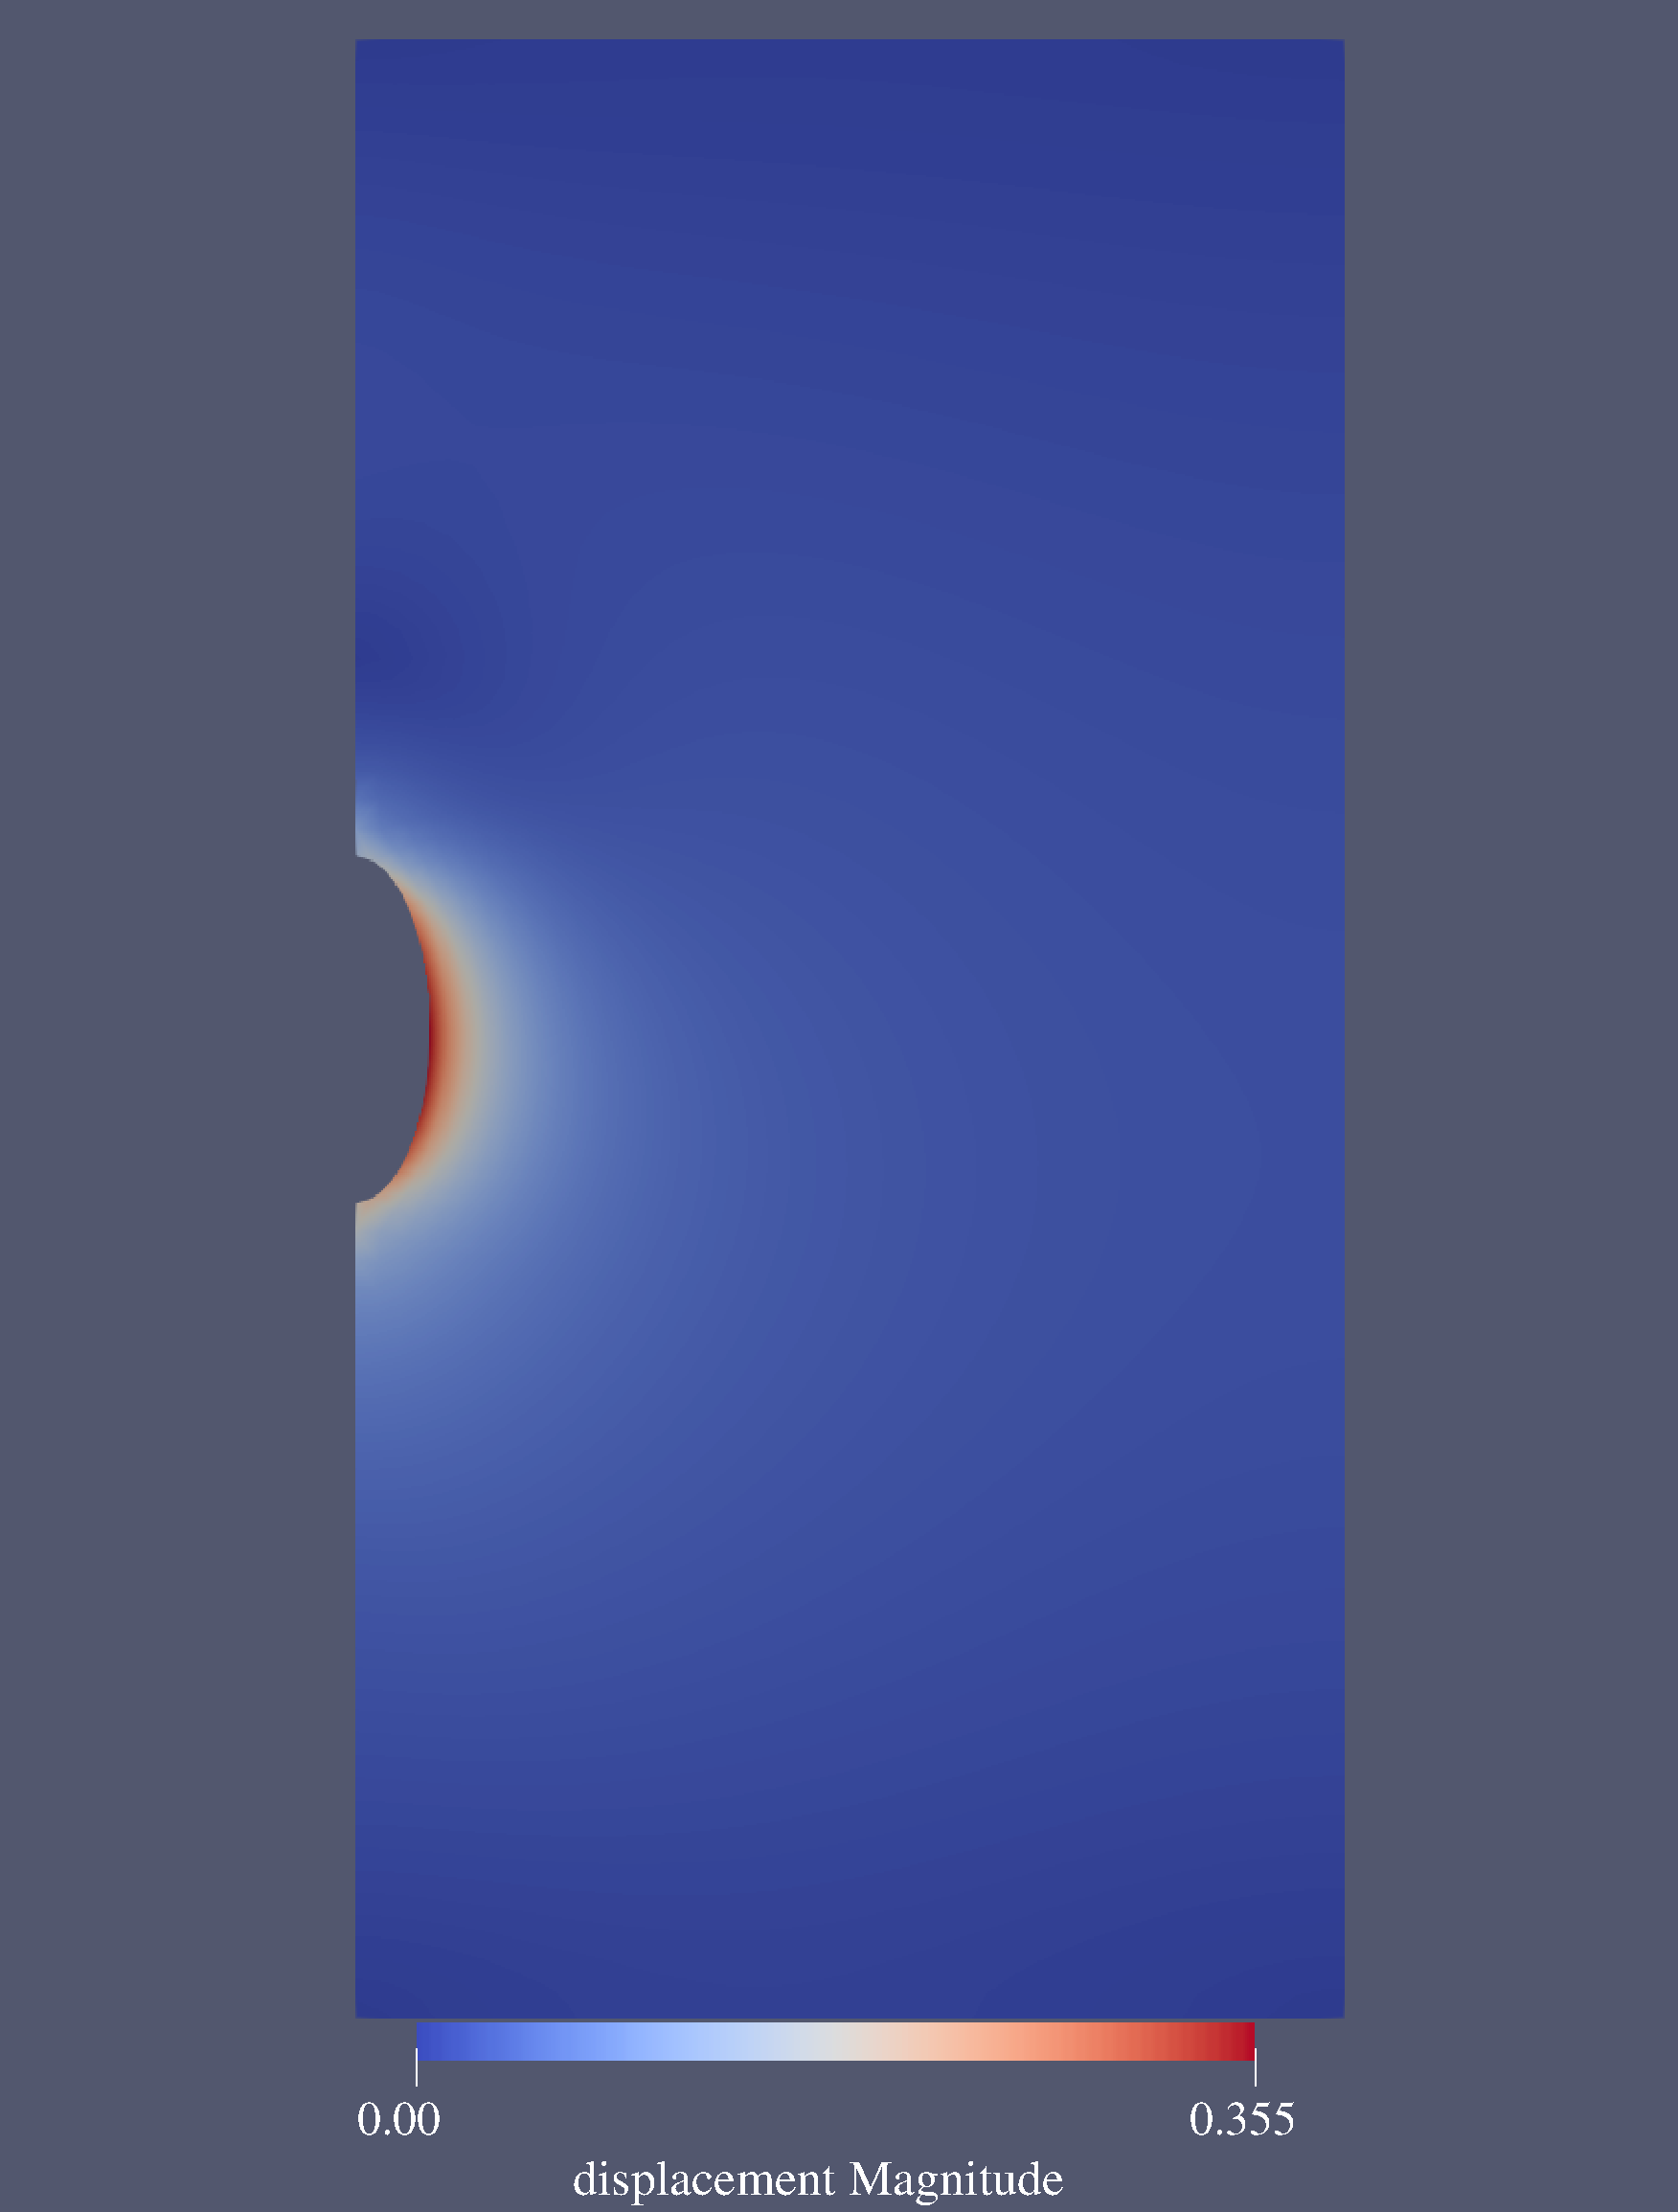
\includegraphics[width=0.95\textwidth]{img/chap5/位移/工况四位移云图.pdf}
        \end{minipage}
    }
    \caption{不同工况下运行十年后位移云图(单位:\si{m})}
    \label{fig:4weiyi}
\end{figure}



如图~\ref{fig:5_34}所示,在腔体围岩的腔顶、腔腰、腔底取A、B、C三个典型位置进行分析。图~\ref{fig:5_20}为不同工况下A、B、C三点位移与时间关系曲线。从图中可以看出,腰部位移最大,其次是底部,顶部位移最小。这是由于腔体呈椭球状,在顶部和底部逐渐收缩,水平方向的应力逐渐相互抵消,因此产生的位移量小于腔体中部。水平应力的相互作用,也会导致围岩挤压而向内收缩,因此应力更大的腔底比腔顶位移大。



\begin{figure}[ht!]
    \centering
    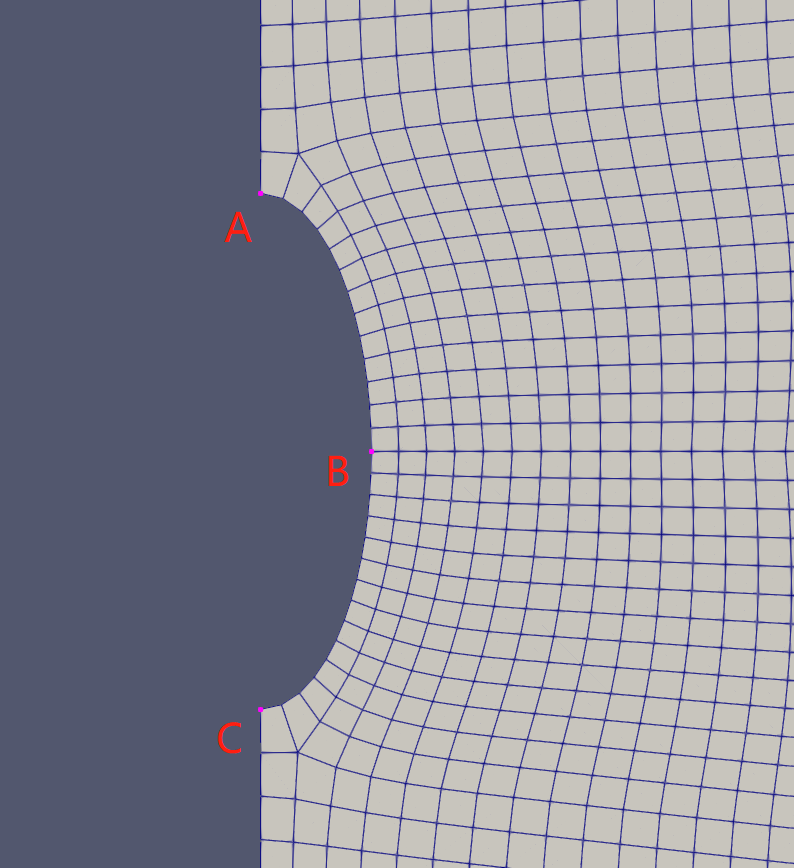
\includegraphics[width=0.6\textwidth]{img/chap5/应力/位置图.png}
    \caption{A、B、C三点位置图}
    \label{fig:5_34}
\end{figure}

\begin{figure}[ht!]
    \centering
    \subfigure[工况一典型位置位移与时间关系曲线]
    {
        \begin{minipage}{7cm}
            \centering
            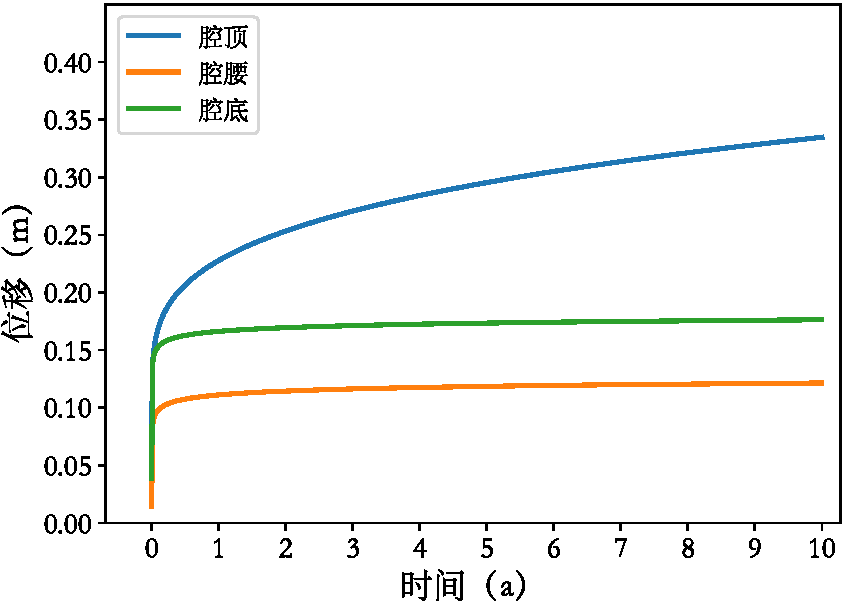
\includegraphics[width=0.95\textwidth]{img/chap5/工况一顶部腰部底部位移与时间关系.pdf}
        \end{minipage}
    }
    \subfigure[工况二典型位置位移与时间关系曲线]
    {
        \begin{minipage}{7cm}
            \centering
            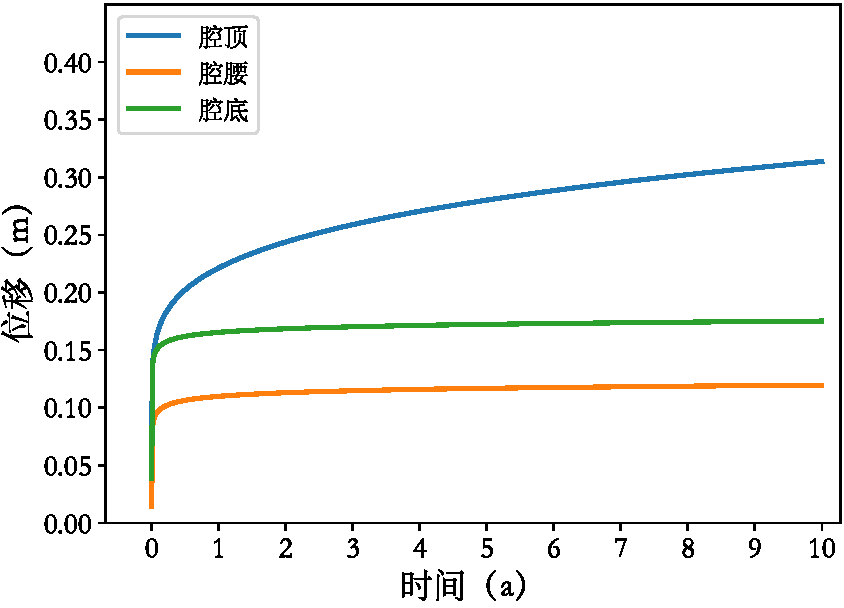
\includegraphics[width=0.95\textwidth]{img/chap5/位移/工况二顶部腰部底部位移与时间关系.pdf}
        \end{minipage}
    }
    \subfigure[工况三典型位置位移与时间关系曲线]
    {
        \begin{minipage}{7cm}
            \centering
            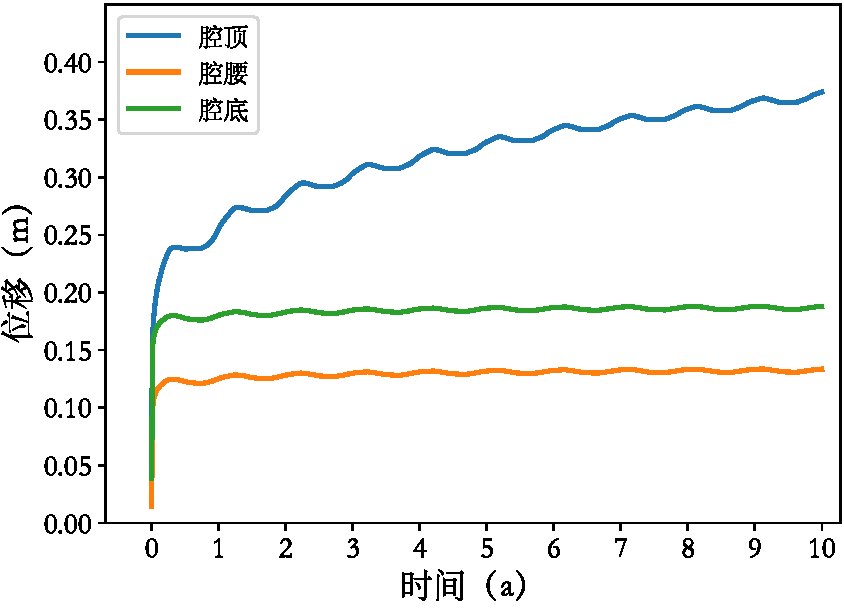
\includegraphics[width=0.95\textwidth]{img/chap5/位移/工况三顶部腰部底部位移与时间关系.pdf}
        \end{minipage}
    }
    \subfigure[工况四典型位置位移与时间关系曲线]
    {
        \begin{minipage}{7cm}
            \centering
            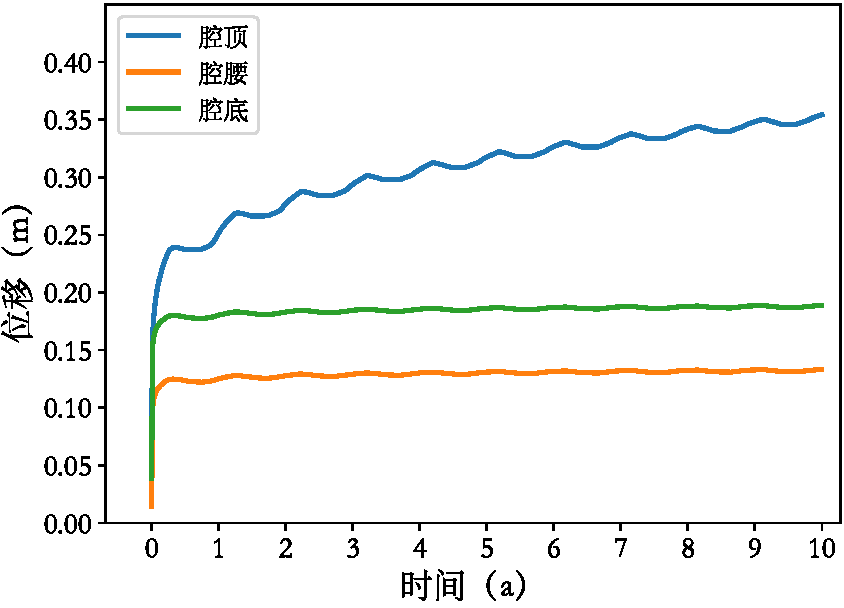
\includegraphics[width=0.95\textwidth]{img/chap5/位移/工况四顶部腰部底部位移与时间关系.pdf}
        \end{minipage}
    }
    \caption{不同工况下典型位置位移与时间关系曲线}
    \label{fig:5_20}
\end{figure}


新能源储库和传统能源储备库的最大位移与时间的关系曲线如图~\ref{fig:5_12}和图~\ref{fig:5_13}所示。计算结果显示,位移随着腔体内压的变化也呈现出周期性增大的趋势。运行的第一年内,位移快速增长,第一年之后位移增加速率变缓,总体成长趋势与运行时间呈现出良好的稳态流变效应。

\begin{figure}[ht!]
    \centering
    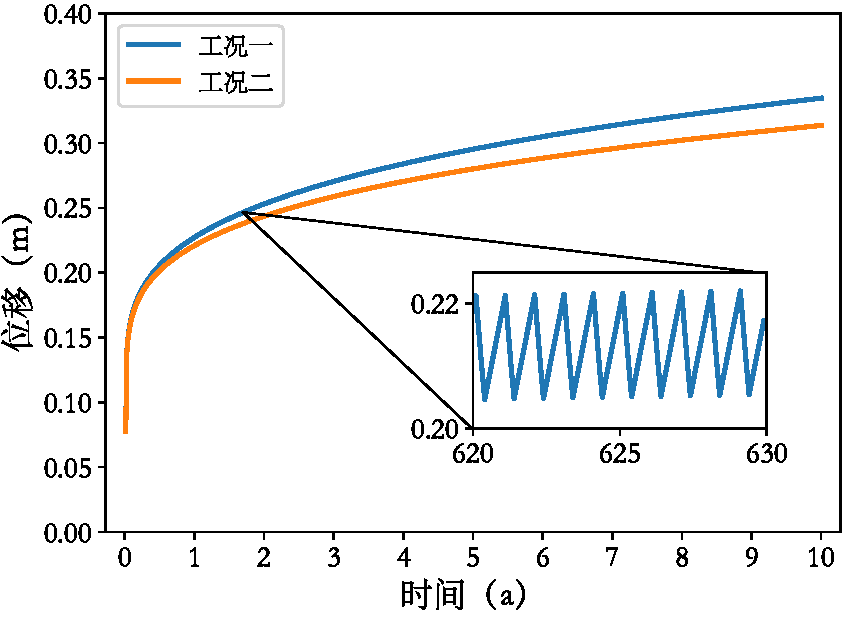
\includegraphics[width=0.55\textwidth]{img/chap5/位移/新能源储库10年最大位移与时间关系.pdf}
    \caption{新能源储库运行\SI{10}{a}后围岩最大位移与时间关系曲线}
    \label{fig:5_12}
\end{figure}

\begin{figure}[ht!]
    \centering
    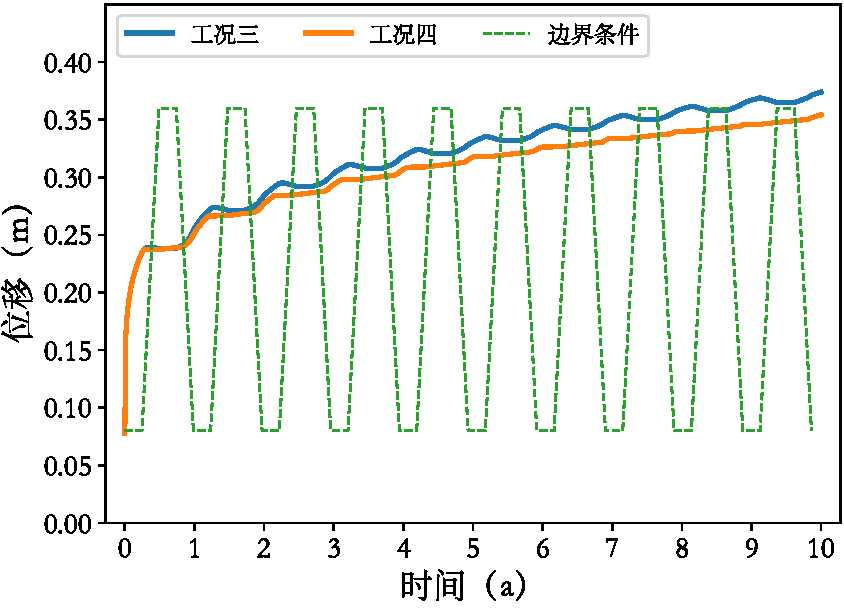
\includegraphics[width=0.55\textwidth]{img/chap5/位移/传统能源储库10年最大位移与时间的关系.pdf}
    \caption{传统能源储库运行\SI{10}{a}后围岩最大位移与时间关系曲线}
    \label{fig:5_13}
\end{figure}

如表~\ref{tab:5_2}所示,不考虑热力耦合的情况下,新能源储库最大位移为\SI{0.315}{m},考虑热力耦合的最大位移为\SI{0.336}{m},差值约为6.6%。不考虑热力耦合的情况下,天然气储库最大位移为\SI{0.355}{m},考虑的热力耦合的最大位移为\SI{0.375}{m},差值约为5.6%。由此可知,新能源储备库的热力学效应引起的变形较传统能源储备库更为显著。因此,对地下盐岩储库长期循环边界条件下运行特性进行研究时,应考虑温度场与应力场之间的相互影响,且循环周期越小,是否考虑热力耦合的差距越明显。

比较工况一和工况三发现,热力耦合下传统能源储库的最大位移(\SI{0.375}{m})大于新能源储库的最大位移(\SI{0.336}{m}),差值约为11.6%,一定程度上可以说明高频注采的运行条件对围岩的整体流变影响不大,甚至抑制了一部分变形量。

\begin{table}[ht!]\small
    \centering
    \begin{tabularx}{\textwidth}{C{1.0}C{1.0}C{1.0}C{1.0}}
        \toprule
        储库类型 & 热力耦合 & 最大位移(m)& 差值(%) \\
        \midrule
        \multirow{2}{*}{新能源储库} & 是  & 0.336 & \multirow{2}{*}{6.6}   \\ 
        &否  & 0.315  &   \\ 
         \midrule
        \multirow{2}{*}{传统能源储备库} & 是  & 0.375 & \multirow{2}{*}{5.6}   \\ 
        &否  & 0.355  &   \\\bottomrule
    \end{tabularx}
    \caption{不同工况下围岩的最大位移(t=3650d)}
    \label{tab:5_2}
\end{table}


\subsection{温度分析}
由理想气体方程可知,气体在压缩或释放的过程中温度会升高或降低。根据拟定工况,储库运行过程中气体温度最高为\SI{378}{K},最低为\SI{323}{K},腔体围岩的初始温度为\SI{323}{K}。因此气体和围岩之间会发生热交换,导致围岩温度上升,长期运行过程中温度向岩石深部传递。

图~\ref{fig:5_21}为不同工况下运行十年后的温度云图和等温线图。从图可以看出,围岩的温度随与溶腔的距离发生均匀变化。运行十年后,新能源储库在长、短半轴的温度影响范围(大于\SI{323}{K})分别是\SI{37}{m}和\SI{47}{m},传统能源储备库温度影响范围分别是\SI{47}{m}和\SI{58}{m},传统能源储备库的温度影响范围稍大,但总体来说影响范围并不大,均小于两倍短轴。

\begin{figure}[ht!]
    \centering
    \subfigure[新能源储库温度云图(t=3650d)]
    {
        \begin{minipage}{7cm}
            \centering
            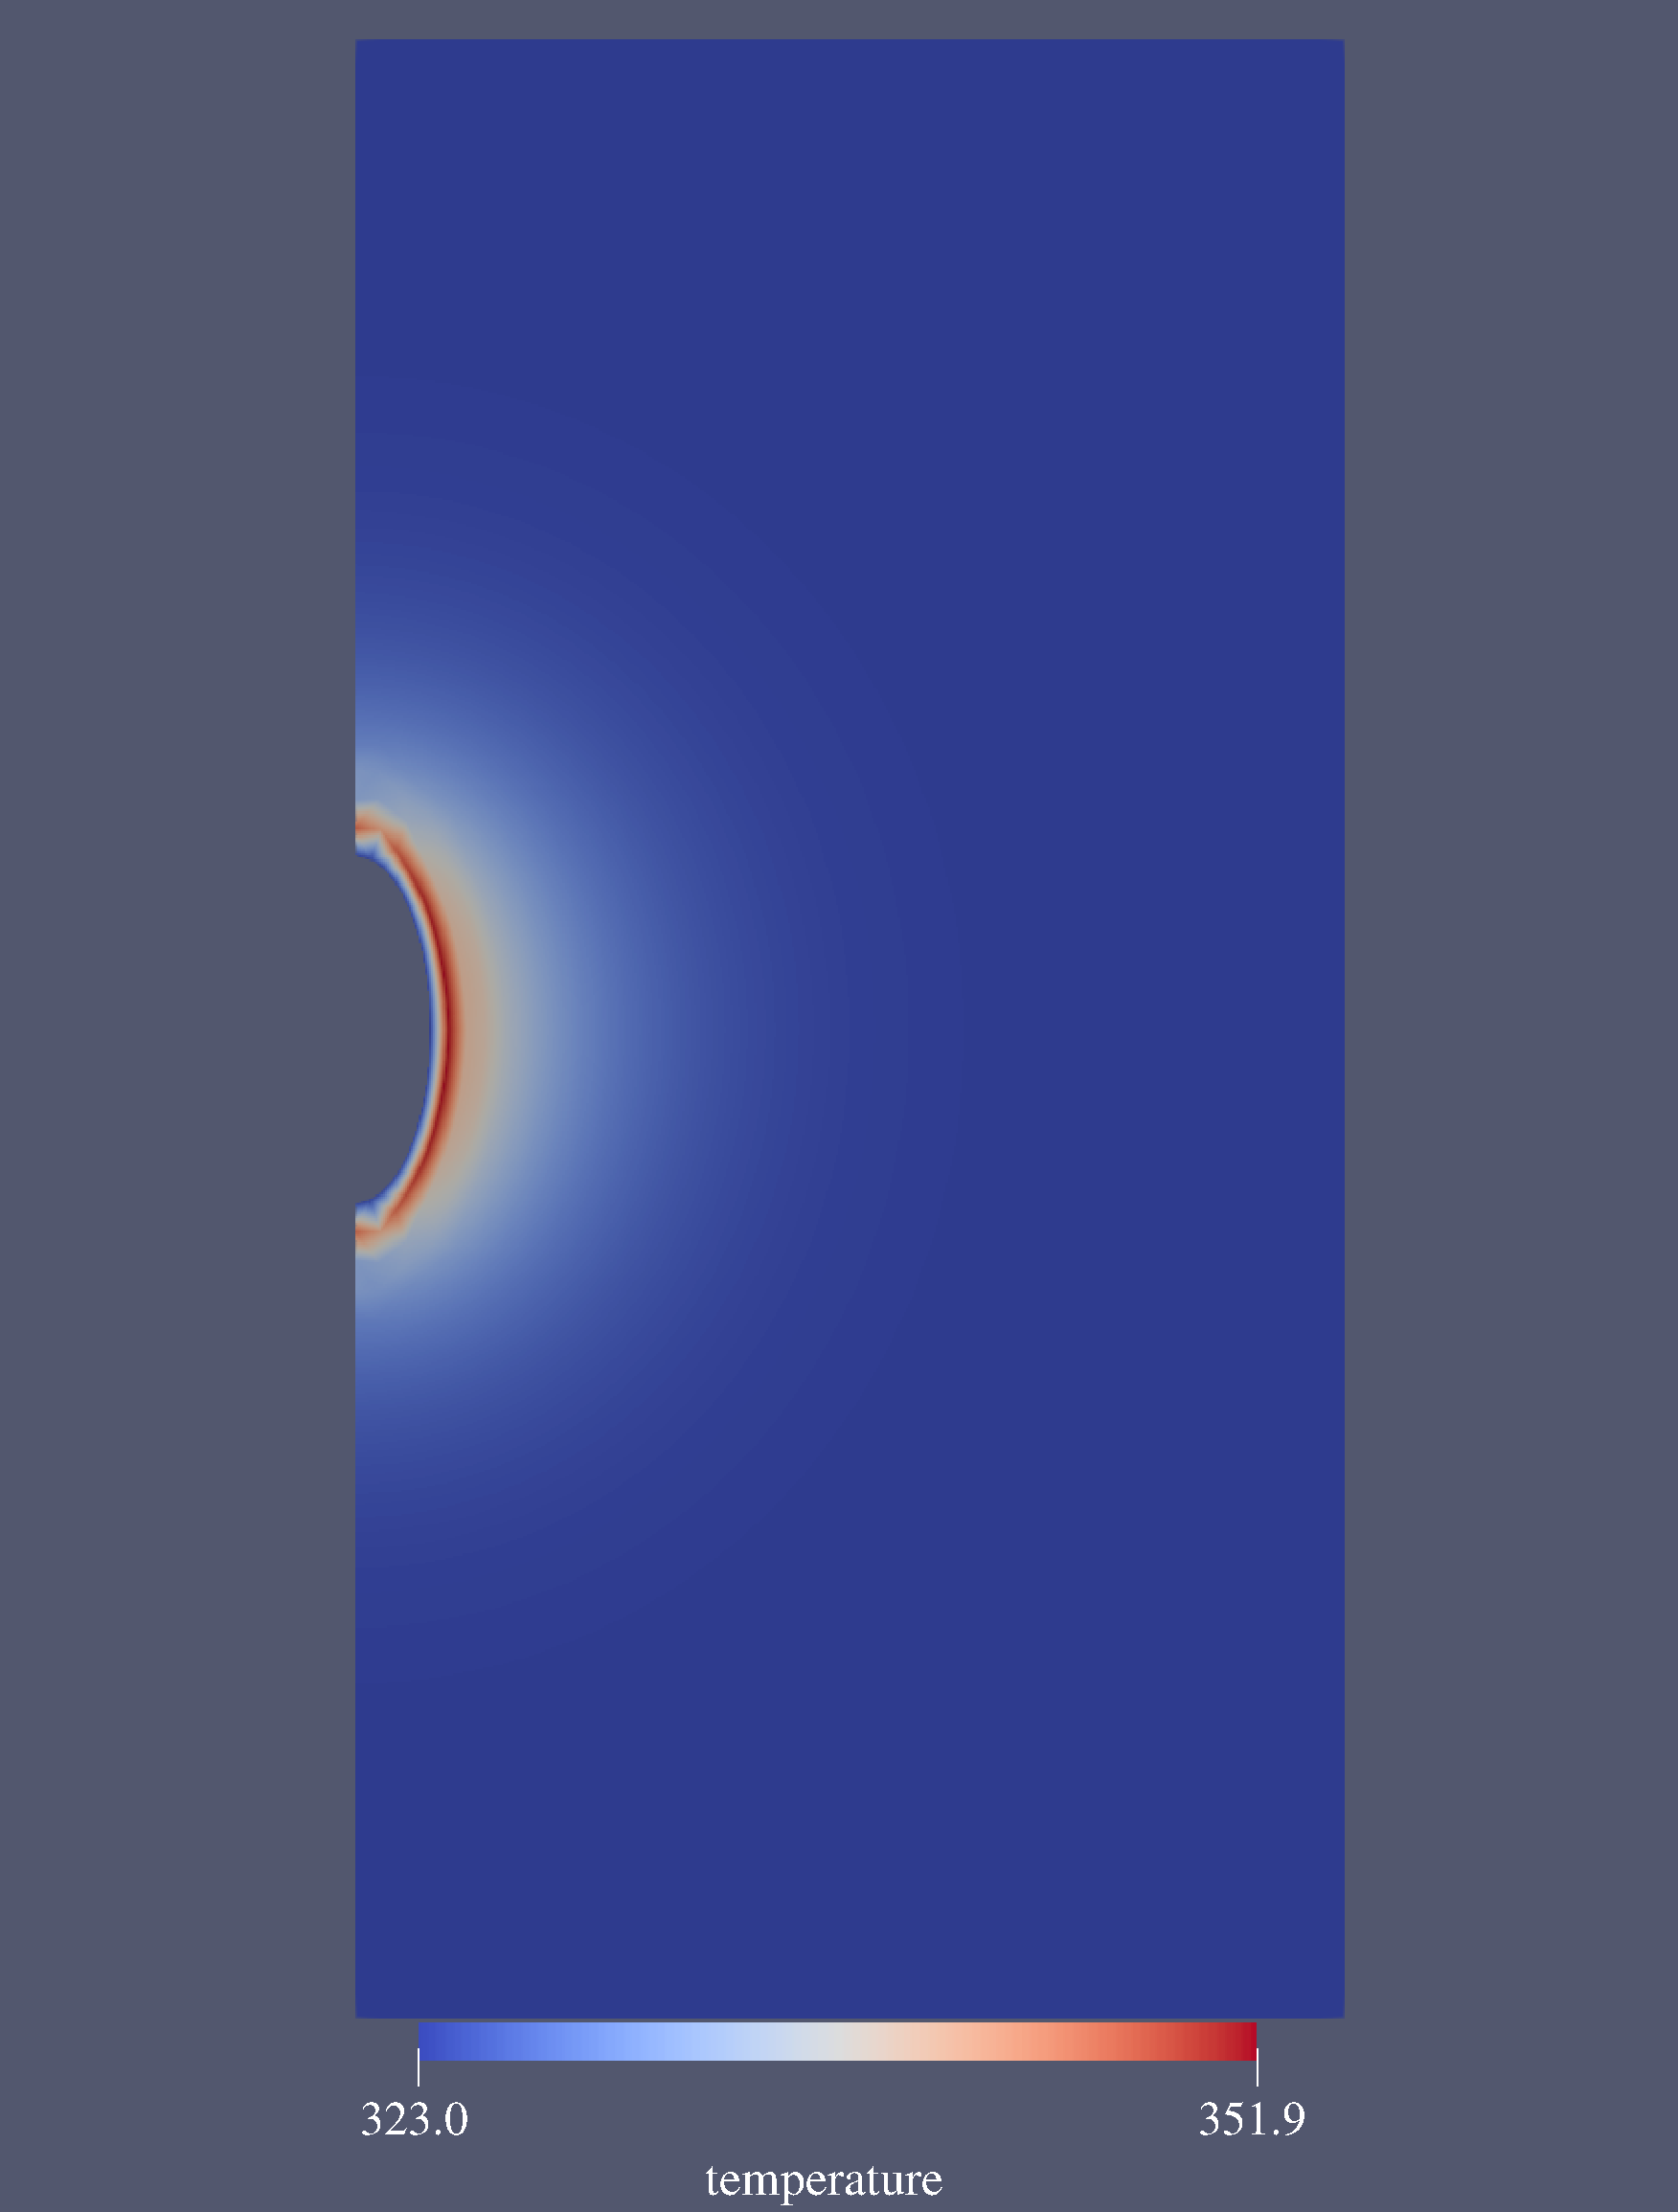
\includegraphics[width=0.95\textwidth]{img/chap5/温度/新能源储库温度云图.pdf}
        \end{minipage}
    }
      \subfigure[新能源储库等温线图(t=3650d)]
    {
        \begin{minipage}{7cm}
            \centering
            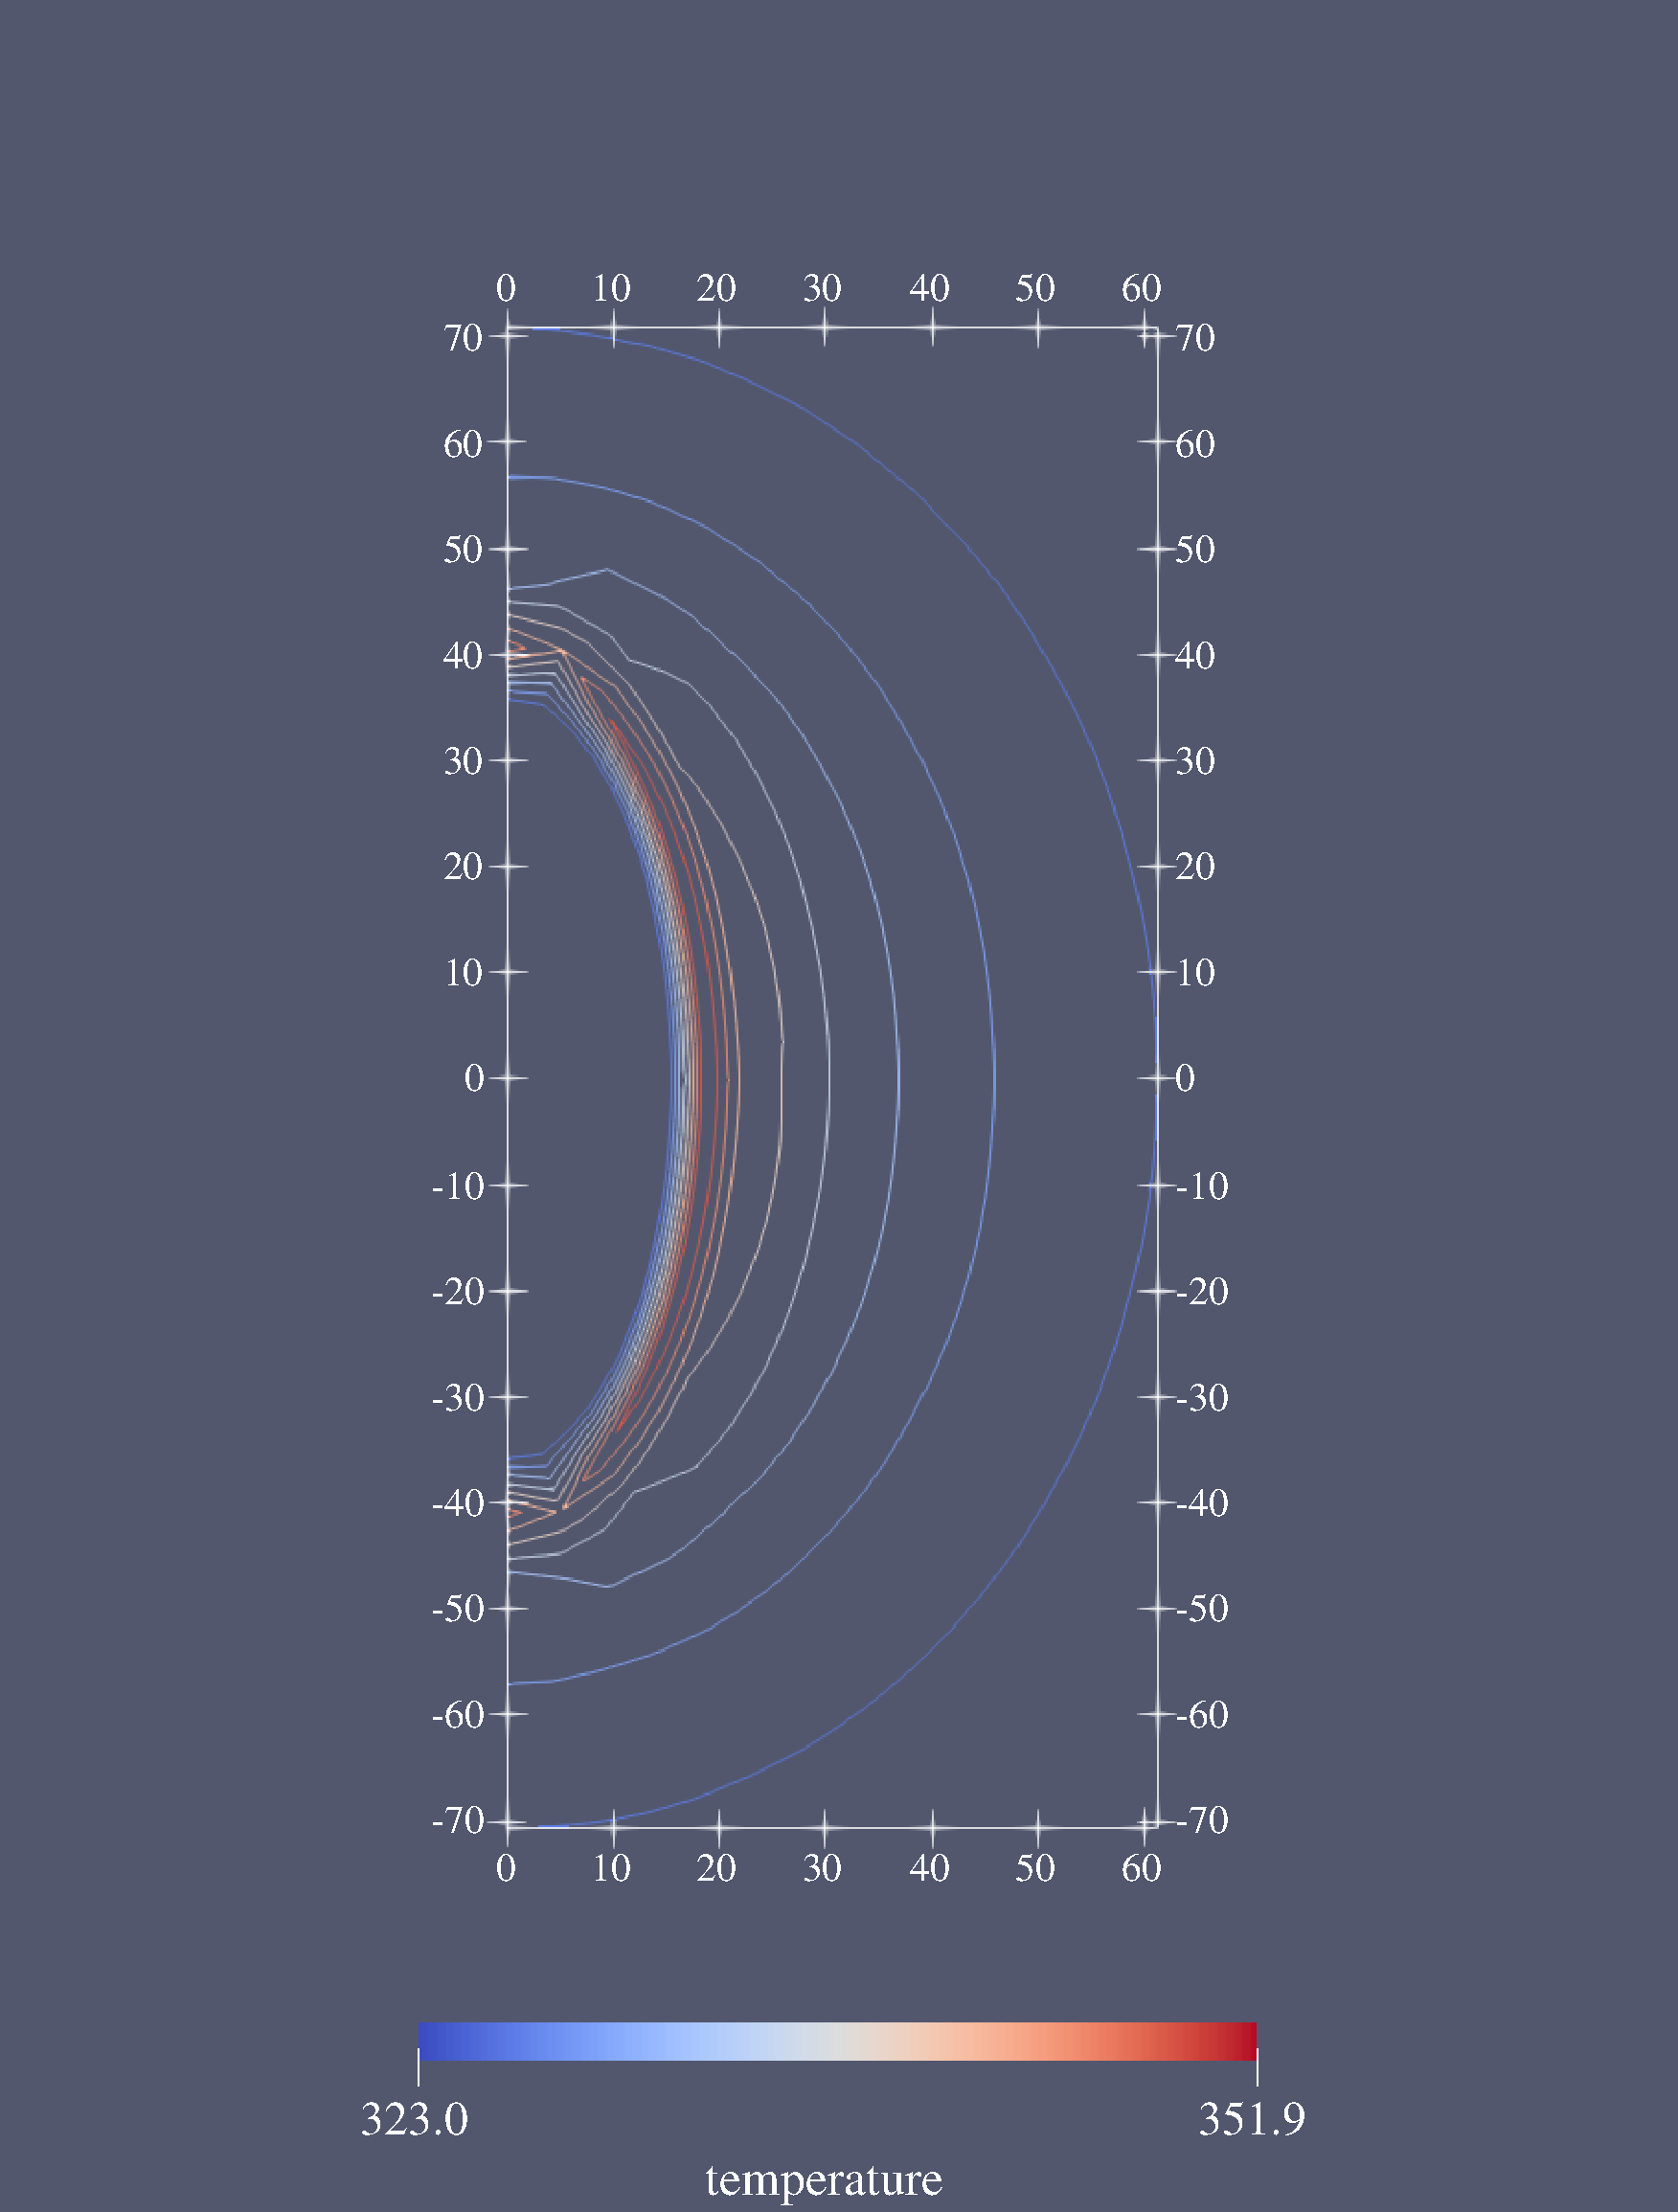
\includegraphics[width=0.95\textwidth]{img/chap5/温度/新能源储库等温线.pdf}
        \end{minipage}
    }
    \subfigure[传统能源储备库温度云图(t=3650d)]
    {
        \begin{minipage}{7cm}
            \centering
            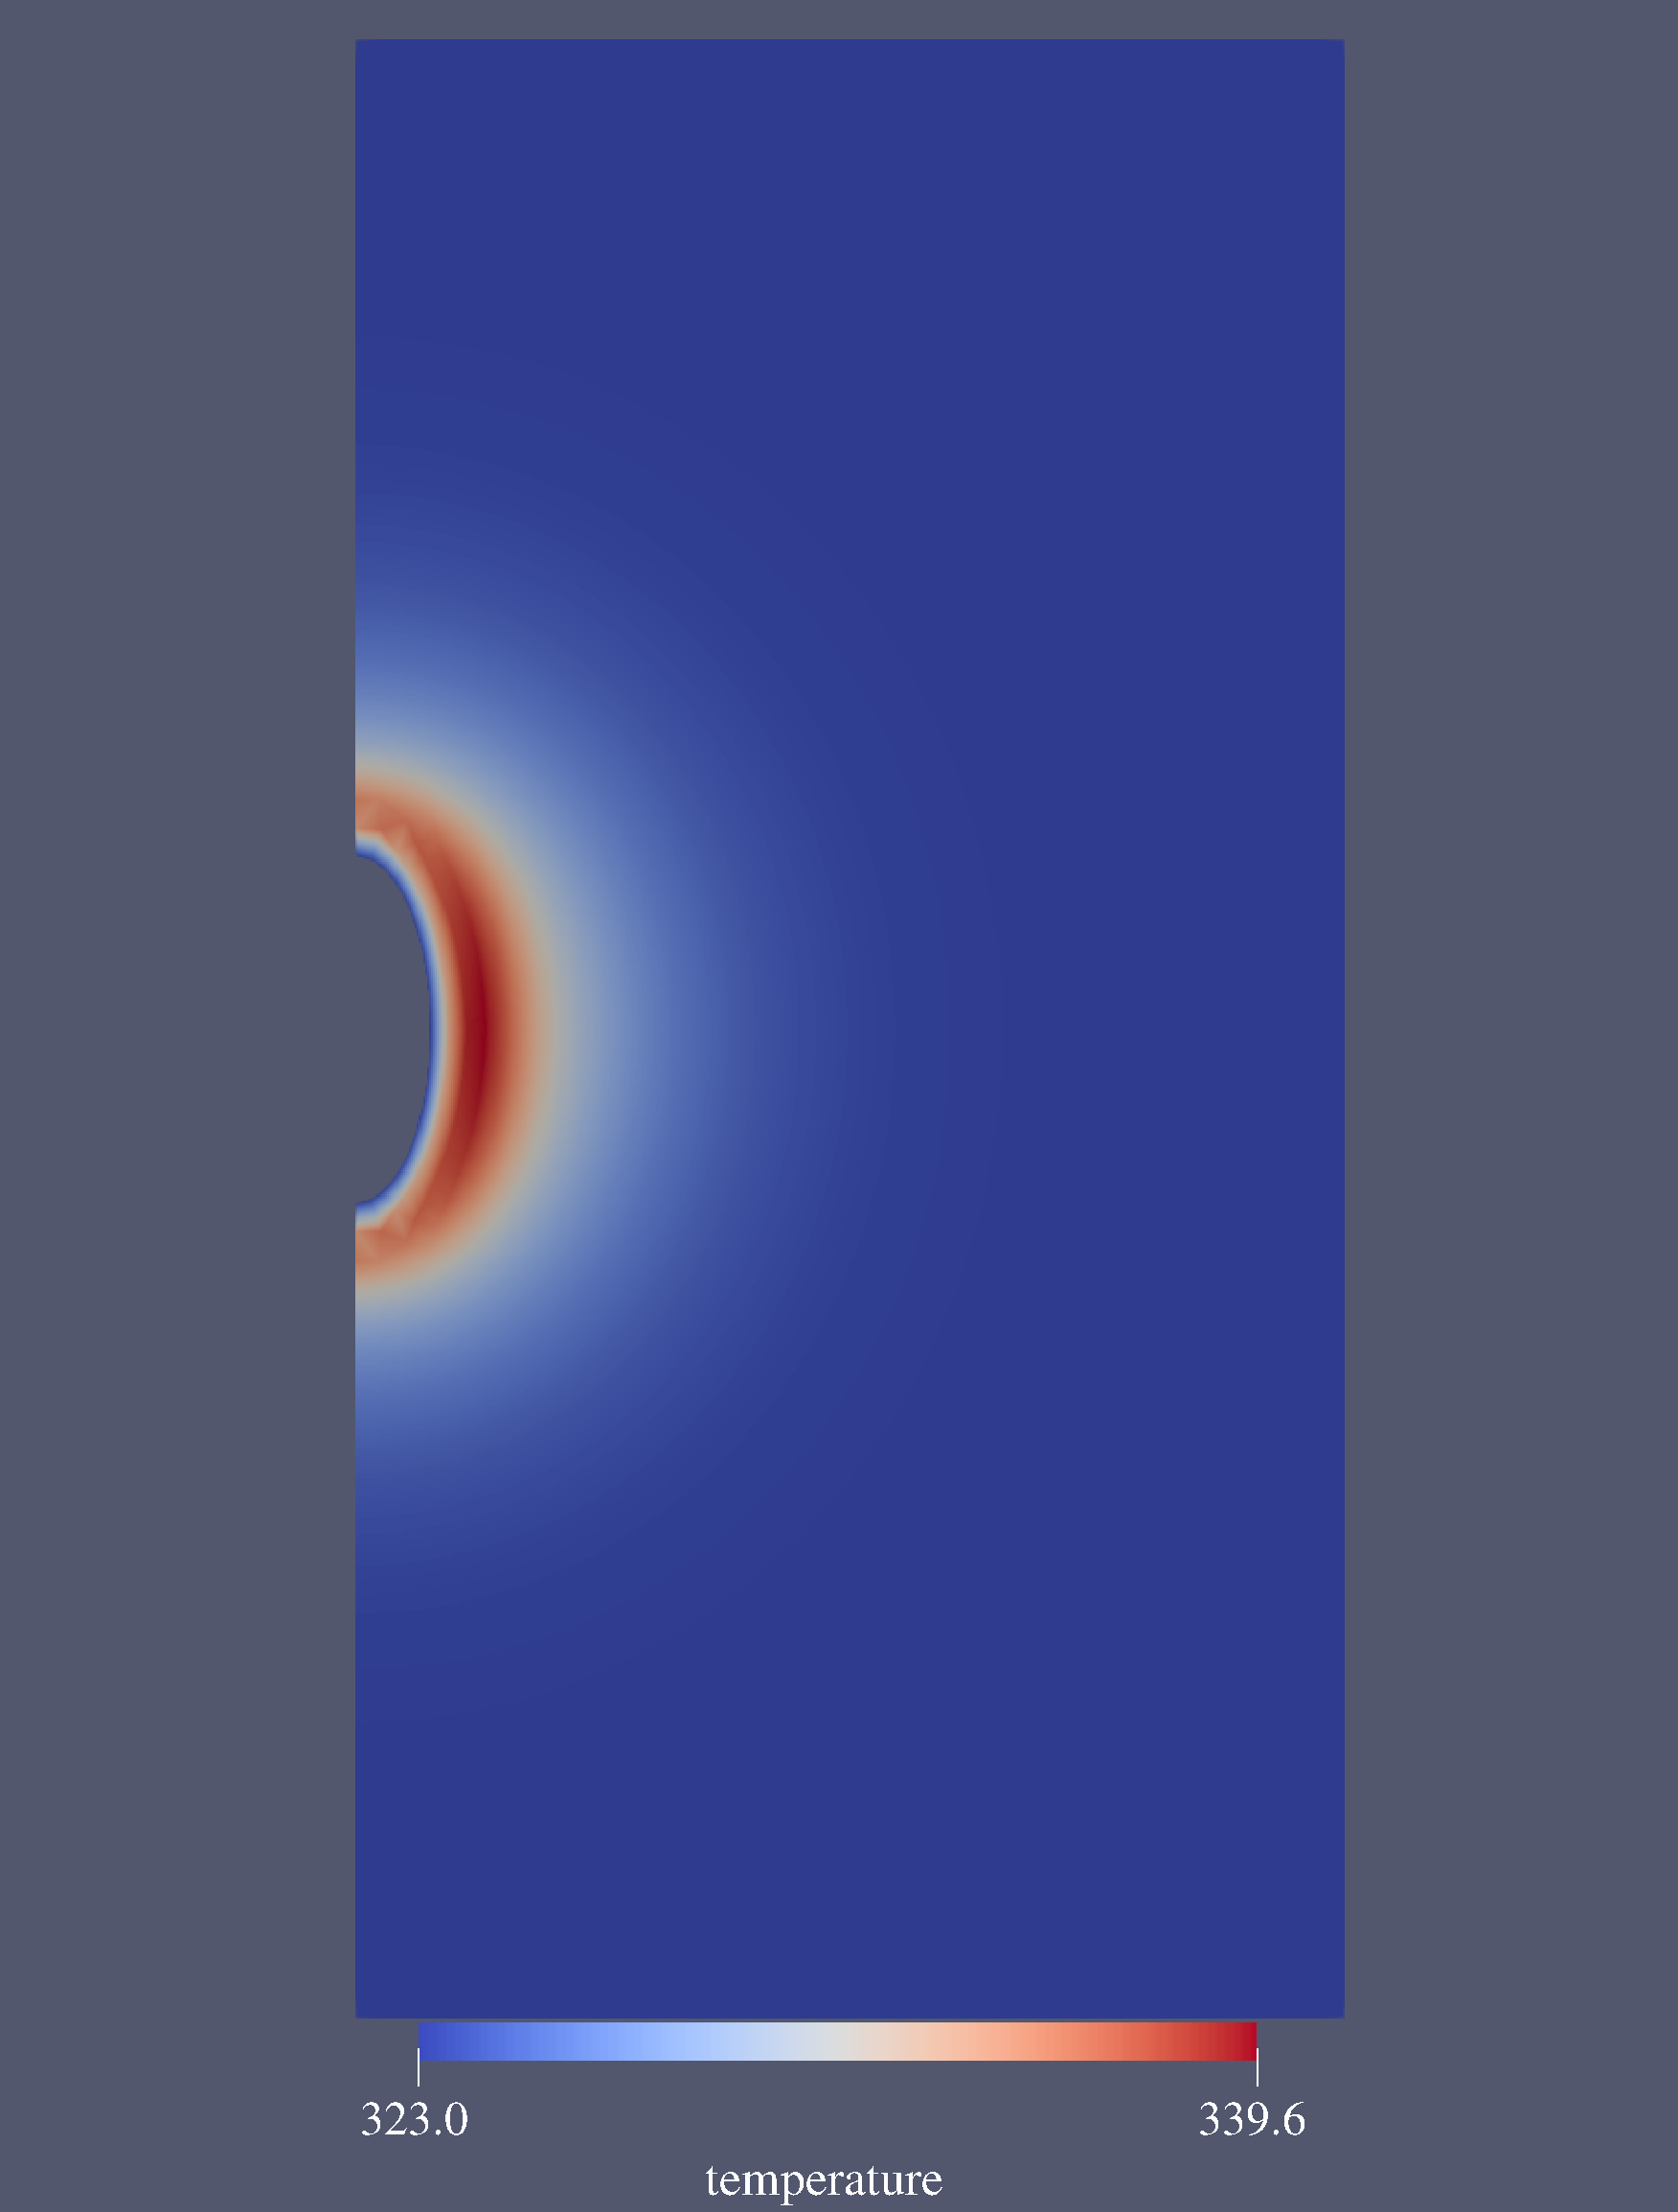
\includegraphics[width=0.95\textwidth]{img/chap5/温度/传统能源储库温度云图.pdf}
        \end{minipage}
    } 
    \subfigure[传统能源储备库等温线图(t=3650d)]
    {
        \begin{minipage}{7cm}
            \centering
            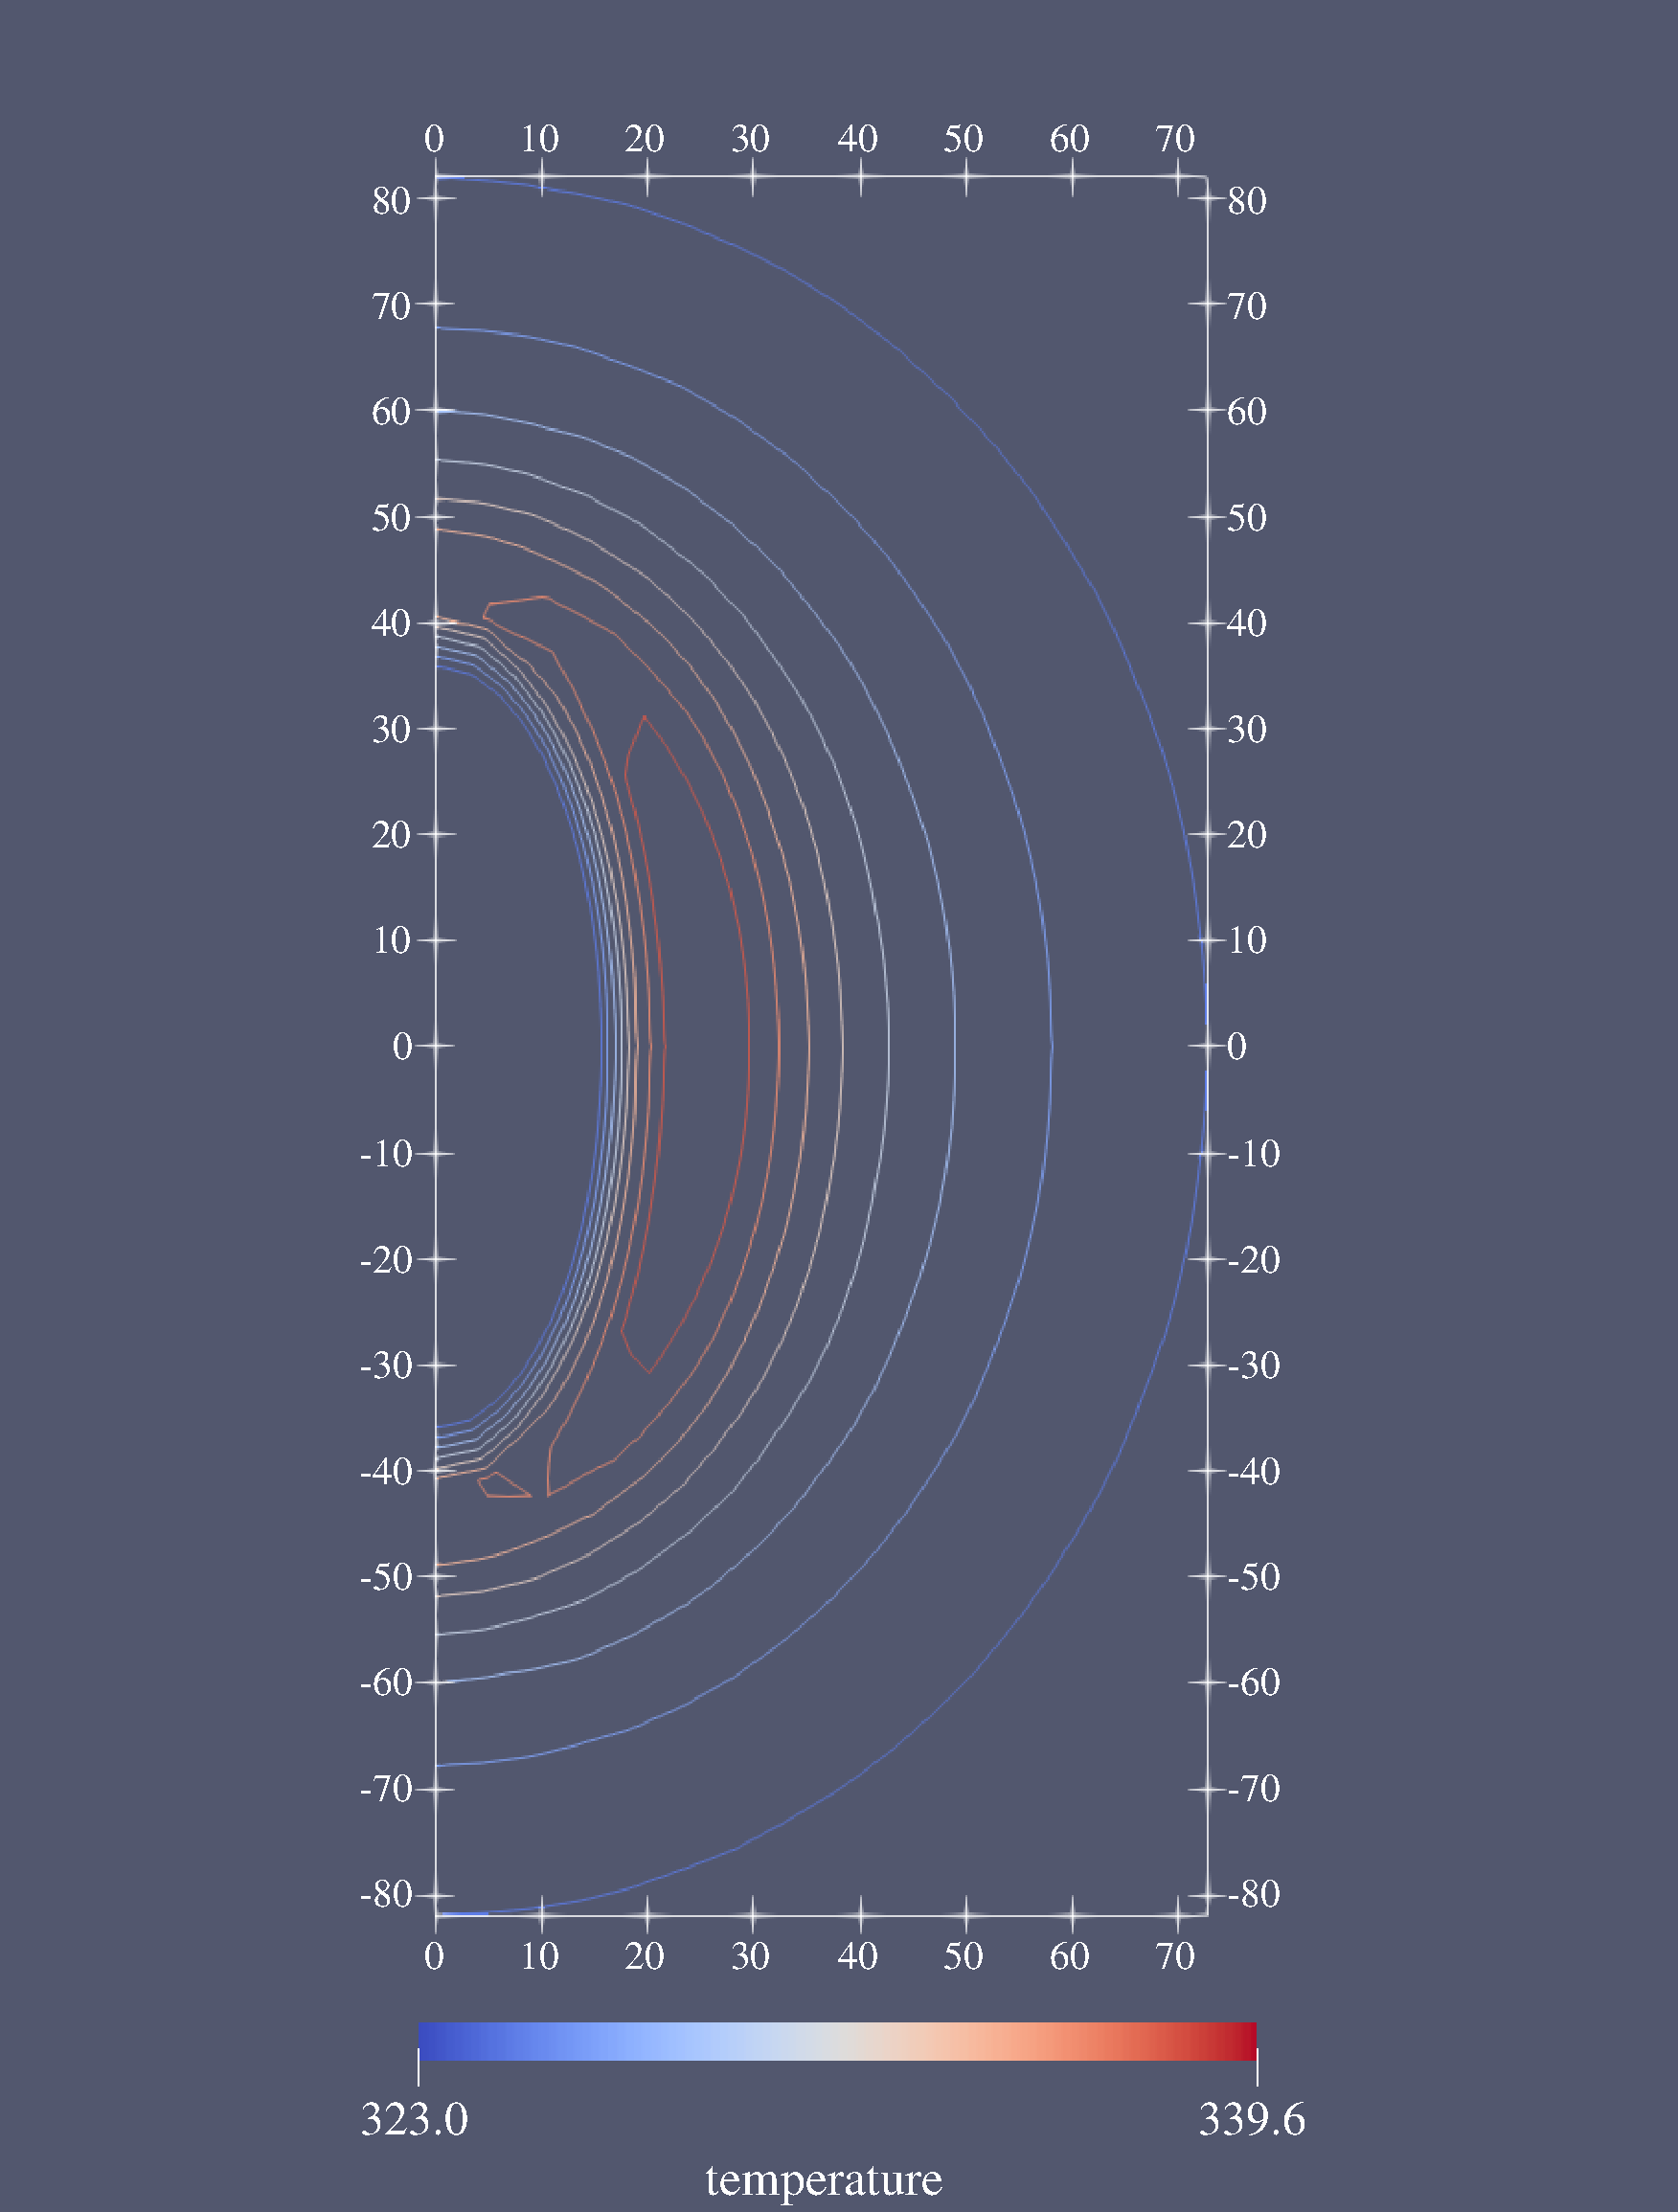
\includegraphics[width=0.95\textwidth]{img/chap5/温度/传统能源储库等温线.pdf}
        \end{minipage}
    }
    \caption{不同储库运行十年温度云图(单位:\si{K})}
    \label{fig:5_21}
\end{figure}

%图~\ref{fig:5_22}为工况一新能源储库围岩运行不同时间后的温度云图,高温围岩集中在一个距溶腔壁约为\SI{5}{m},约为\SI{3}{m}厚的岩层中,随着运行时间的增加内高温带宽度缓慢增加,并逐渐向更深层的盐岩传递温度。



温度边界相同的情况下运行十年后(t=3650d),新能源储库围岩最高温度为\SI{351.9}{K},传统能源储备库围岩最高温度为\SI{339.6}{K}。但传统能源储备库在每个周期的恒定高压阶段(每个周期6月-9月),达到最高温度,为\SI{378.0}{K}。这是由于新能源储库的温度循环周期极短,而热量从气体传至围岩需要一定的时间,因此当围岩温度在上升的过程中,储库就进入采气阶段,气体温度迅速下降,导致围岩温度并不能达到气体的最高温度。相对于新能源储库来说,传统能源储库的循环周期很长,热量有足够的时间能够从气体中传至围岩,因此在围岩的温度随着气体温度的升高而升高,在注气阶段结束的时候就达到\SI{378.0}{K}(腔内气体温度上限)。从温度云图中也可看出,一个运行周期结束时处于传统能源储备库的采气阶段,溶腔附近的围岩温度很低,与气体温度相近。

图\ref{fig:5_33}为新能源储库中最高温度与时间的关系曲线,储库运行一年内温度急剧上升,从第三年开始最高温度保持不变。图\ref{fig:5_35}为温度影响范围随时间的变化关系曲线,由图可以看出,储库运行第一年温度影响范围迅速扩大,随后几年温度影响范围随运行时间线性增大。

\begin{figure}[ht!]
    \centering
    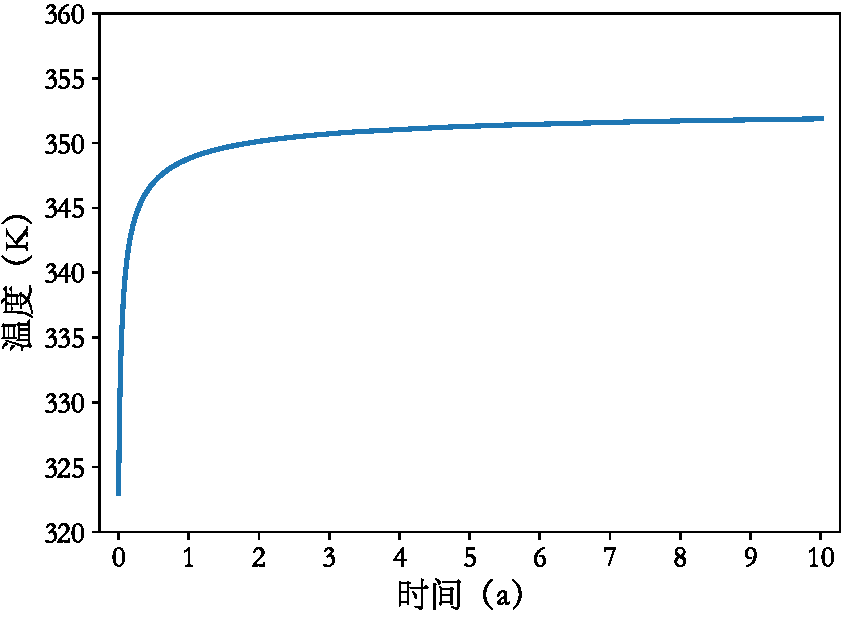
\includegraphics[width=0.55\textwidth]{img/chap5/温度/新能源储库最高温度与时间的关系.pdf}
    \caption{新能源储库围岩最高温度随时间的关系曲线}
    \label{fig:5_33}
\end{figure}

\begin{figure}[ht!]
    \centering
    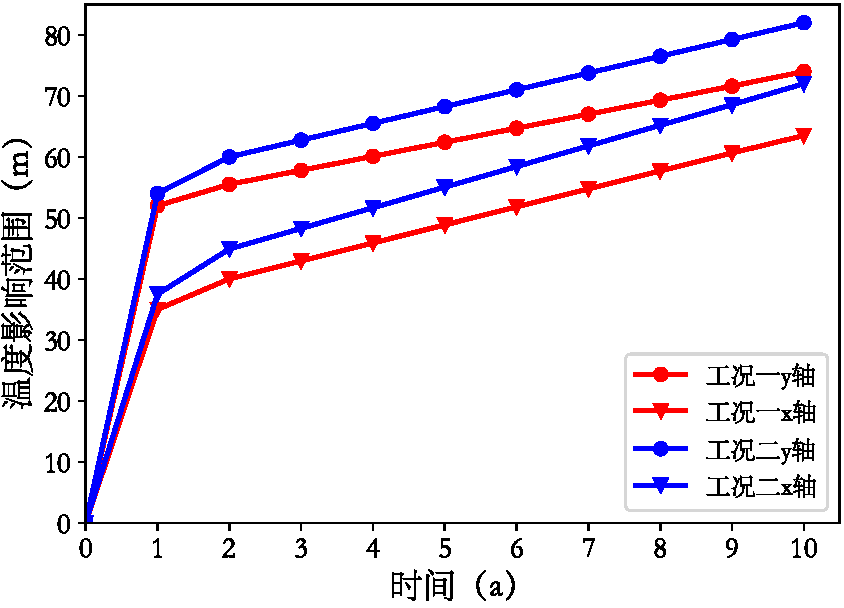
\includegraphics[width=0.55\textwidth]{img/chap5/温度/温度影响范围随时间的关系曲线.pdf}
    \caption{温度影响范围随时间的关系曲线}
    \label{fig:5_35}
\end{figure}

由上述模拟结果可见,温度循环周期较长的传统能源储备库产生的温差相较于新能源储库更大,从而产生更大的热应力。相对于传统能源储库,新能源储库围岩的高温范围相对集中,温度对盐岩力学性能的影响相对较小。但实际工程分析中,不论是新能源储库还是传统能源储库,都应该充分考虑其不同特点的热应力对储库长期运行的不同影响;对于传统能源储库温度更应注意多腔体之间或单腔体与其他构筑物之间的温度的相互影响。

\subsection{应力分析}

根据物体热胀冷缩的原理,当物体所处环境温度变化时,体积会随之发生变化。理论分析状态下,物体不受限制可自由变化,此时只产生热应变,物体内部不产生热应力。但在实际工程分析中,物理往往受到内部和外部的多重约束,发生热应变的同时产生热应力。

在储库进行注气的过程中,气体温度升高,溶腔附近的围岩受热而膨胀,并对深处的低温围岩产生压应力;在储库进行采气的过程中,热量由高温的围岩流向气体,溶腔附近围岩发生收缩对深处围岩产生拉应力。又由于温度的周期性变化,导致围岩内部产生热应力也发生周期性变化。同时,围岩还受到溶腔中周期变化的气体压力、地层压力的共同作用,当产生的总应力过大时,围岩内部产生损伤,在长期运行的过程中导致腔体收缩、破坏,影响储库的正常使用\cite{解宁2019地下盐穴储气库盐岩热损伤机理}。

不同工况下围岩Von Mises应力云图如图~\ref{fig:5_39}所示。从云图中可以看出,任何工况下,都会在腔腰部分出现应力集中现象,而腔顶和腔底部分的应力相对较小。各工况运行\SI{10}{a}后,腔顶、腔腰和腔底的最大应力列于表\ref{tab:5_10}。通过比较具体应力数值可以发现:(1)同等运行工况下,新能源储库的各位置的最大Mises等效应力都大于传统能源储库;(2)考虑热力耦合的情况下,新能源储库腔顶和腔底部分的Mises应力有7%-10%的增大,而腔腰部分的应力有所减小;传统能源储库在考虑热力耦合的效应下各位置最大应力略有减小(约为1%-2%);(3)相同边界条件下,新能源储库的最大应力相较于传统能源储库的增长幅度可达18%-22%,循环周期的长短对于储库围岩应力的影响十分明显;(4)新能源出库腔腰位置的最大等效应力约为腔顶和腔底位置的1.4倍,略大于传统能源储的1.3倍,因此新能源储库的应力集中现象
更为明显。%\todoZN{不要写不大,写提高了多少百分比}


\begin{figure}[ht!]
    \centering
    \subfigure[工况一运行\SI{10}{a}后Von Mises应力云图]
    {
        \begin{minipage}{7cm}
            \centering
            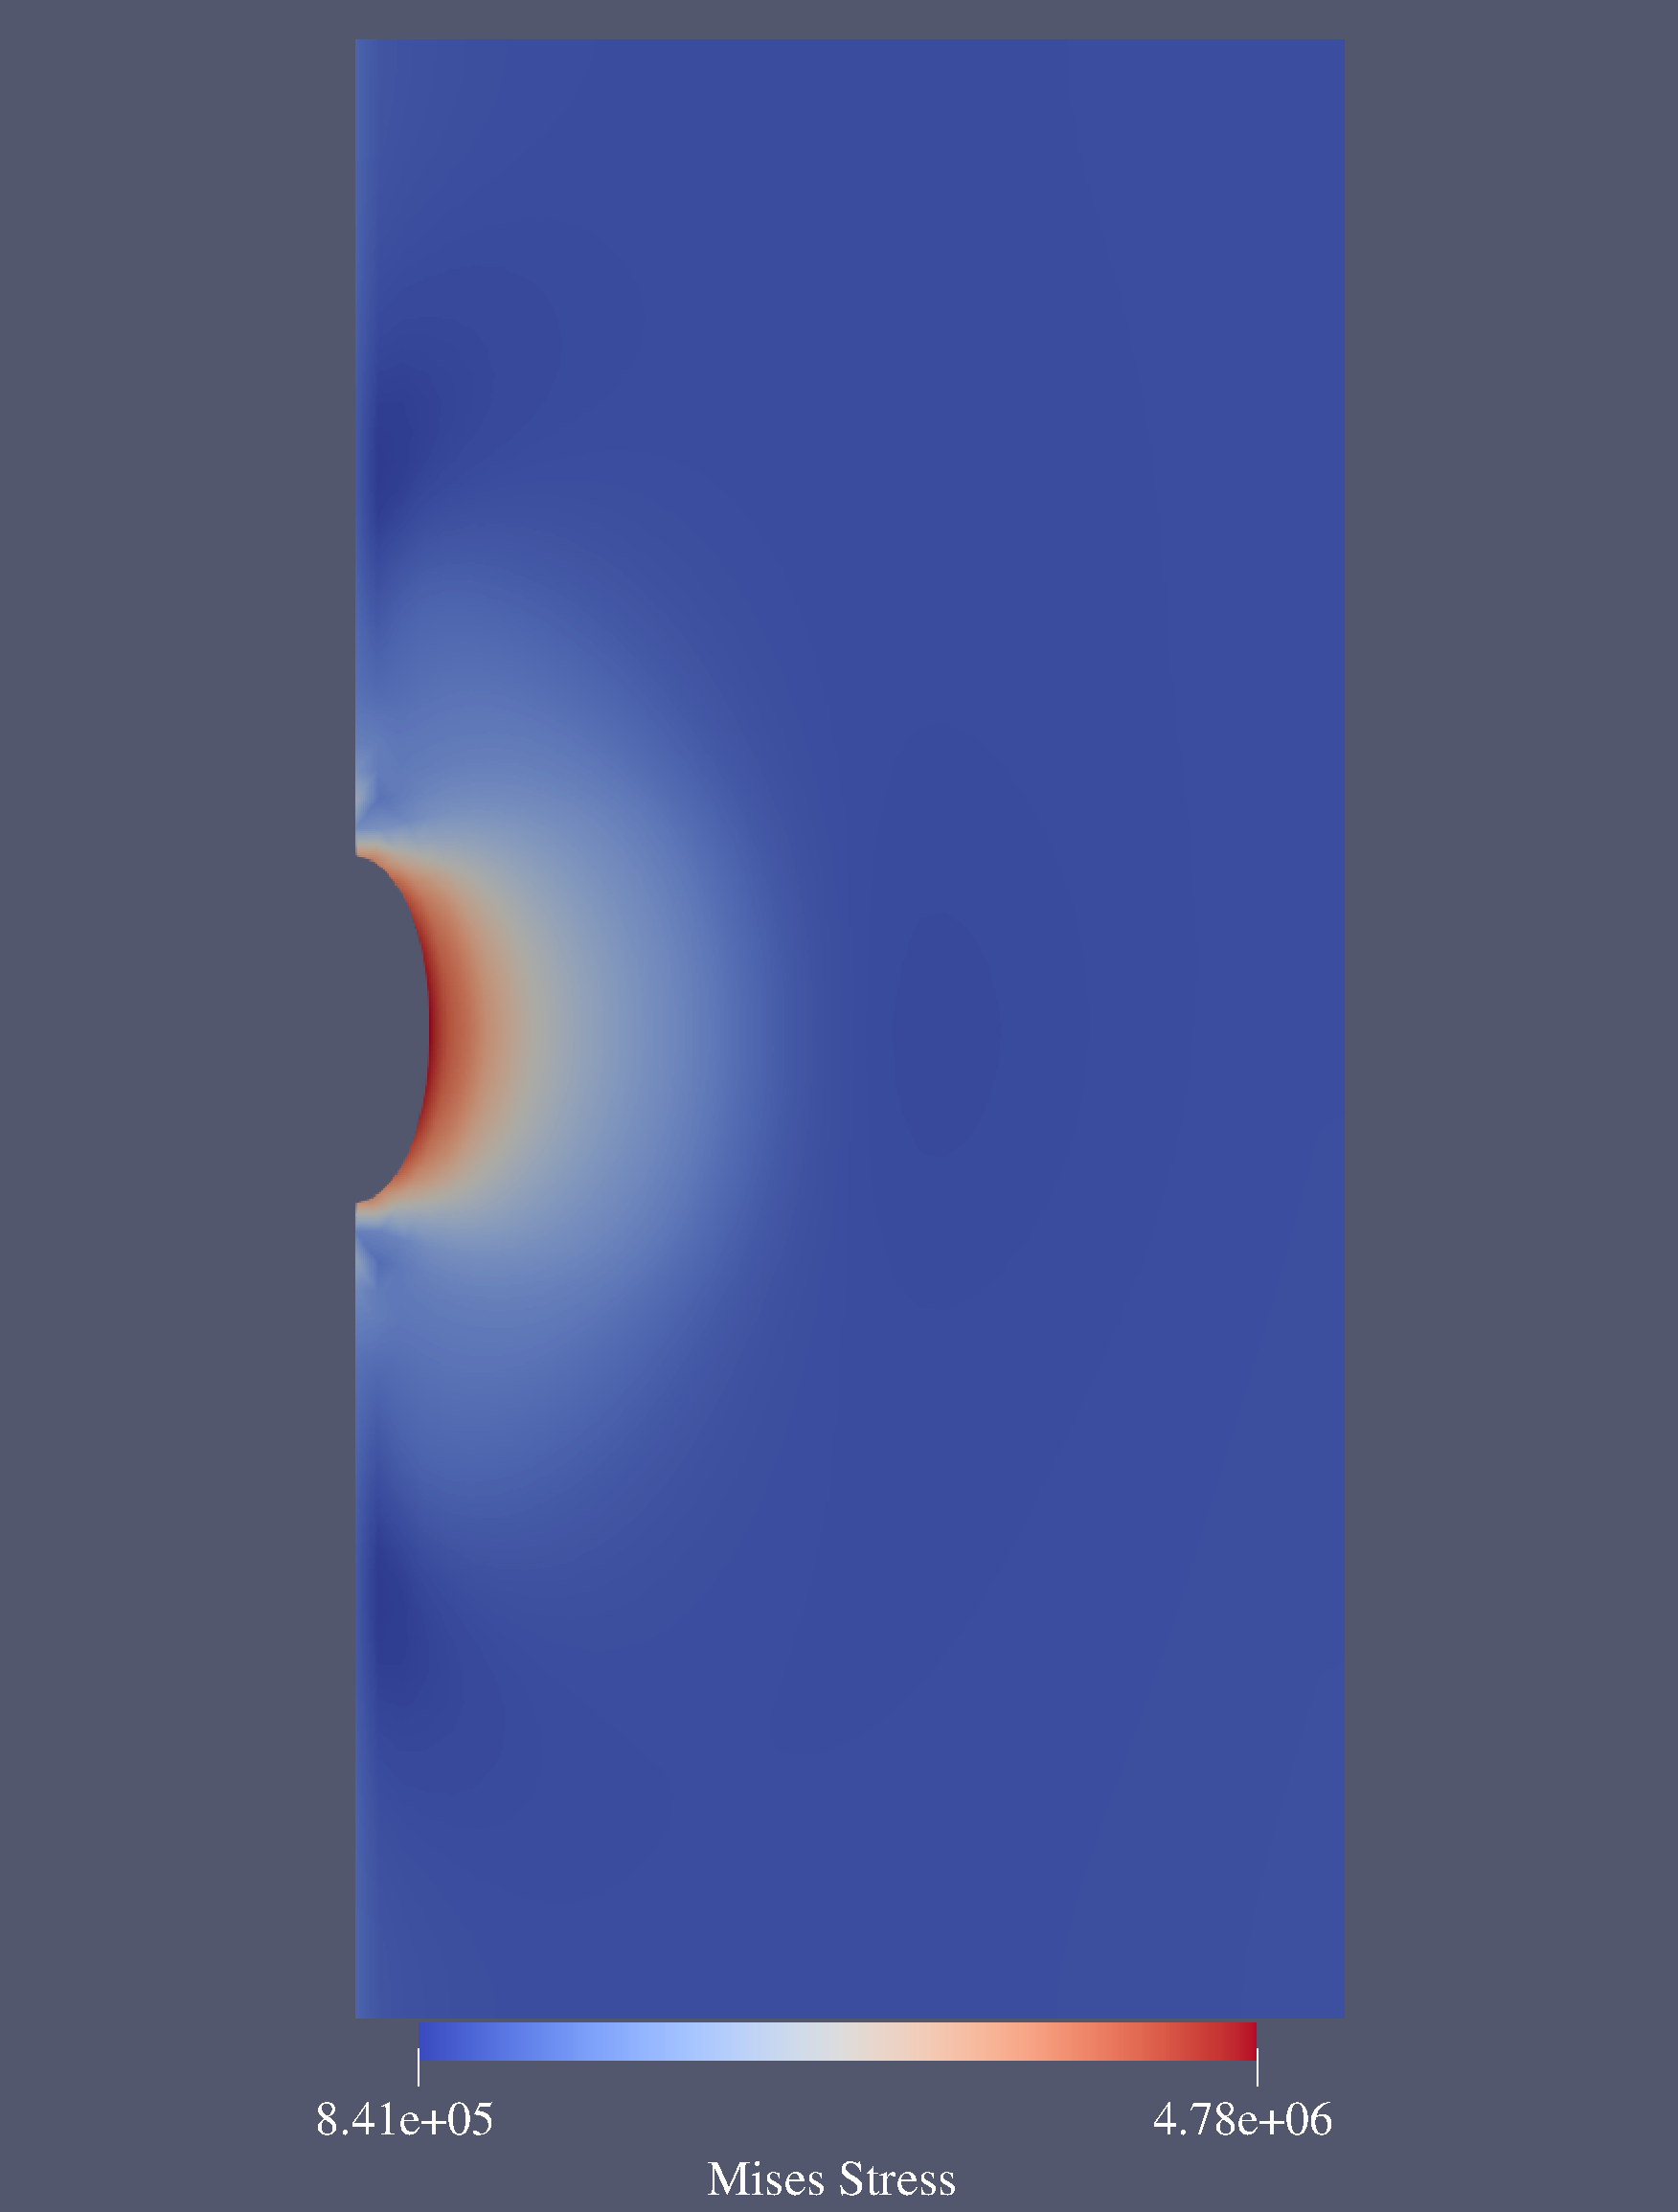
\includegraphics[width=0.95\textwidth]{img/chap5/应力/gk1mises.pdf}
        \end{minipage}
    }
      \subfigure[工况二运行\SI{10}{a}后Von Mises应力云图]
    {
        \begin{minipage}{7cm}
            \centering
            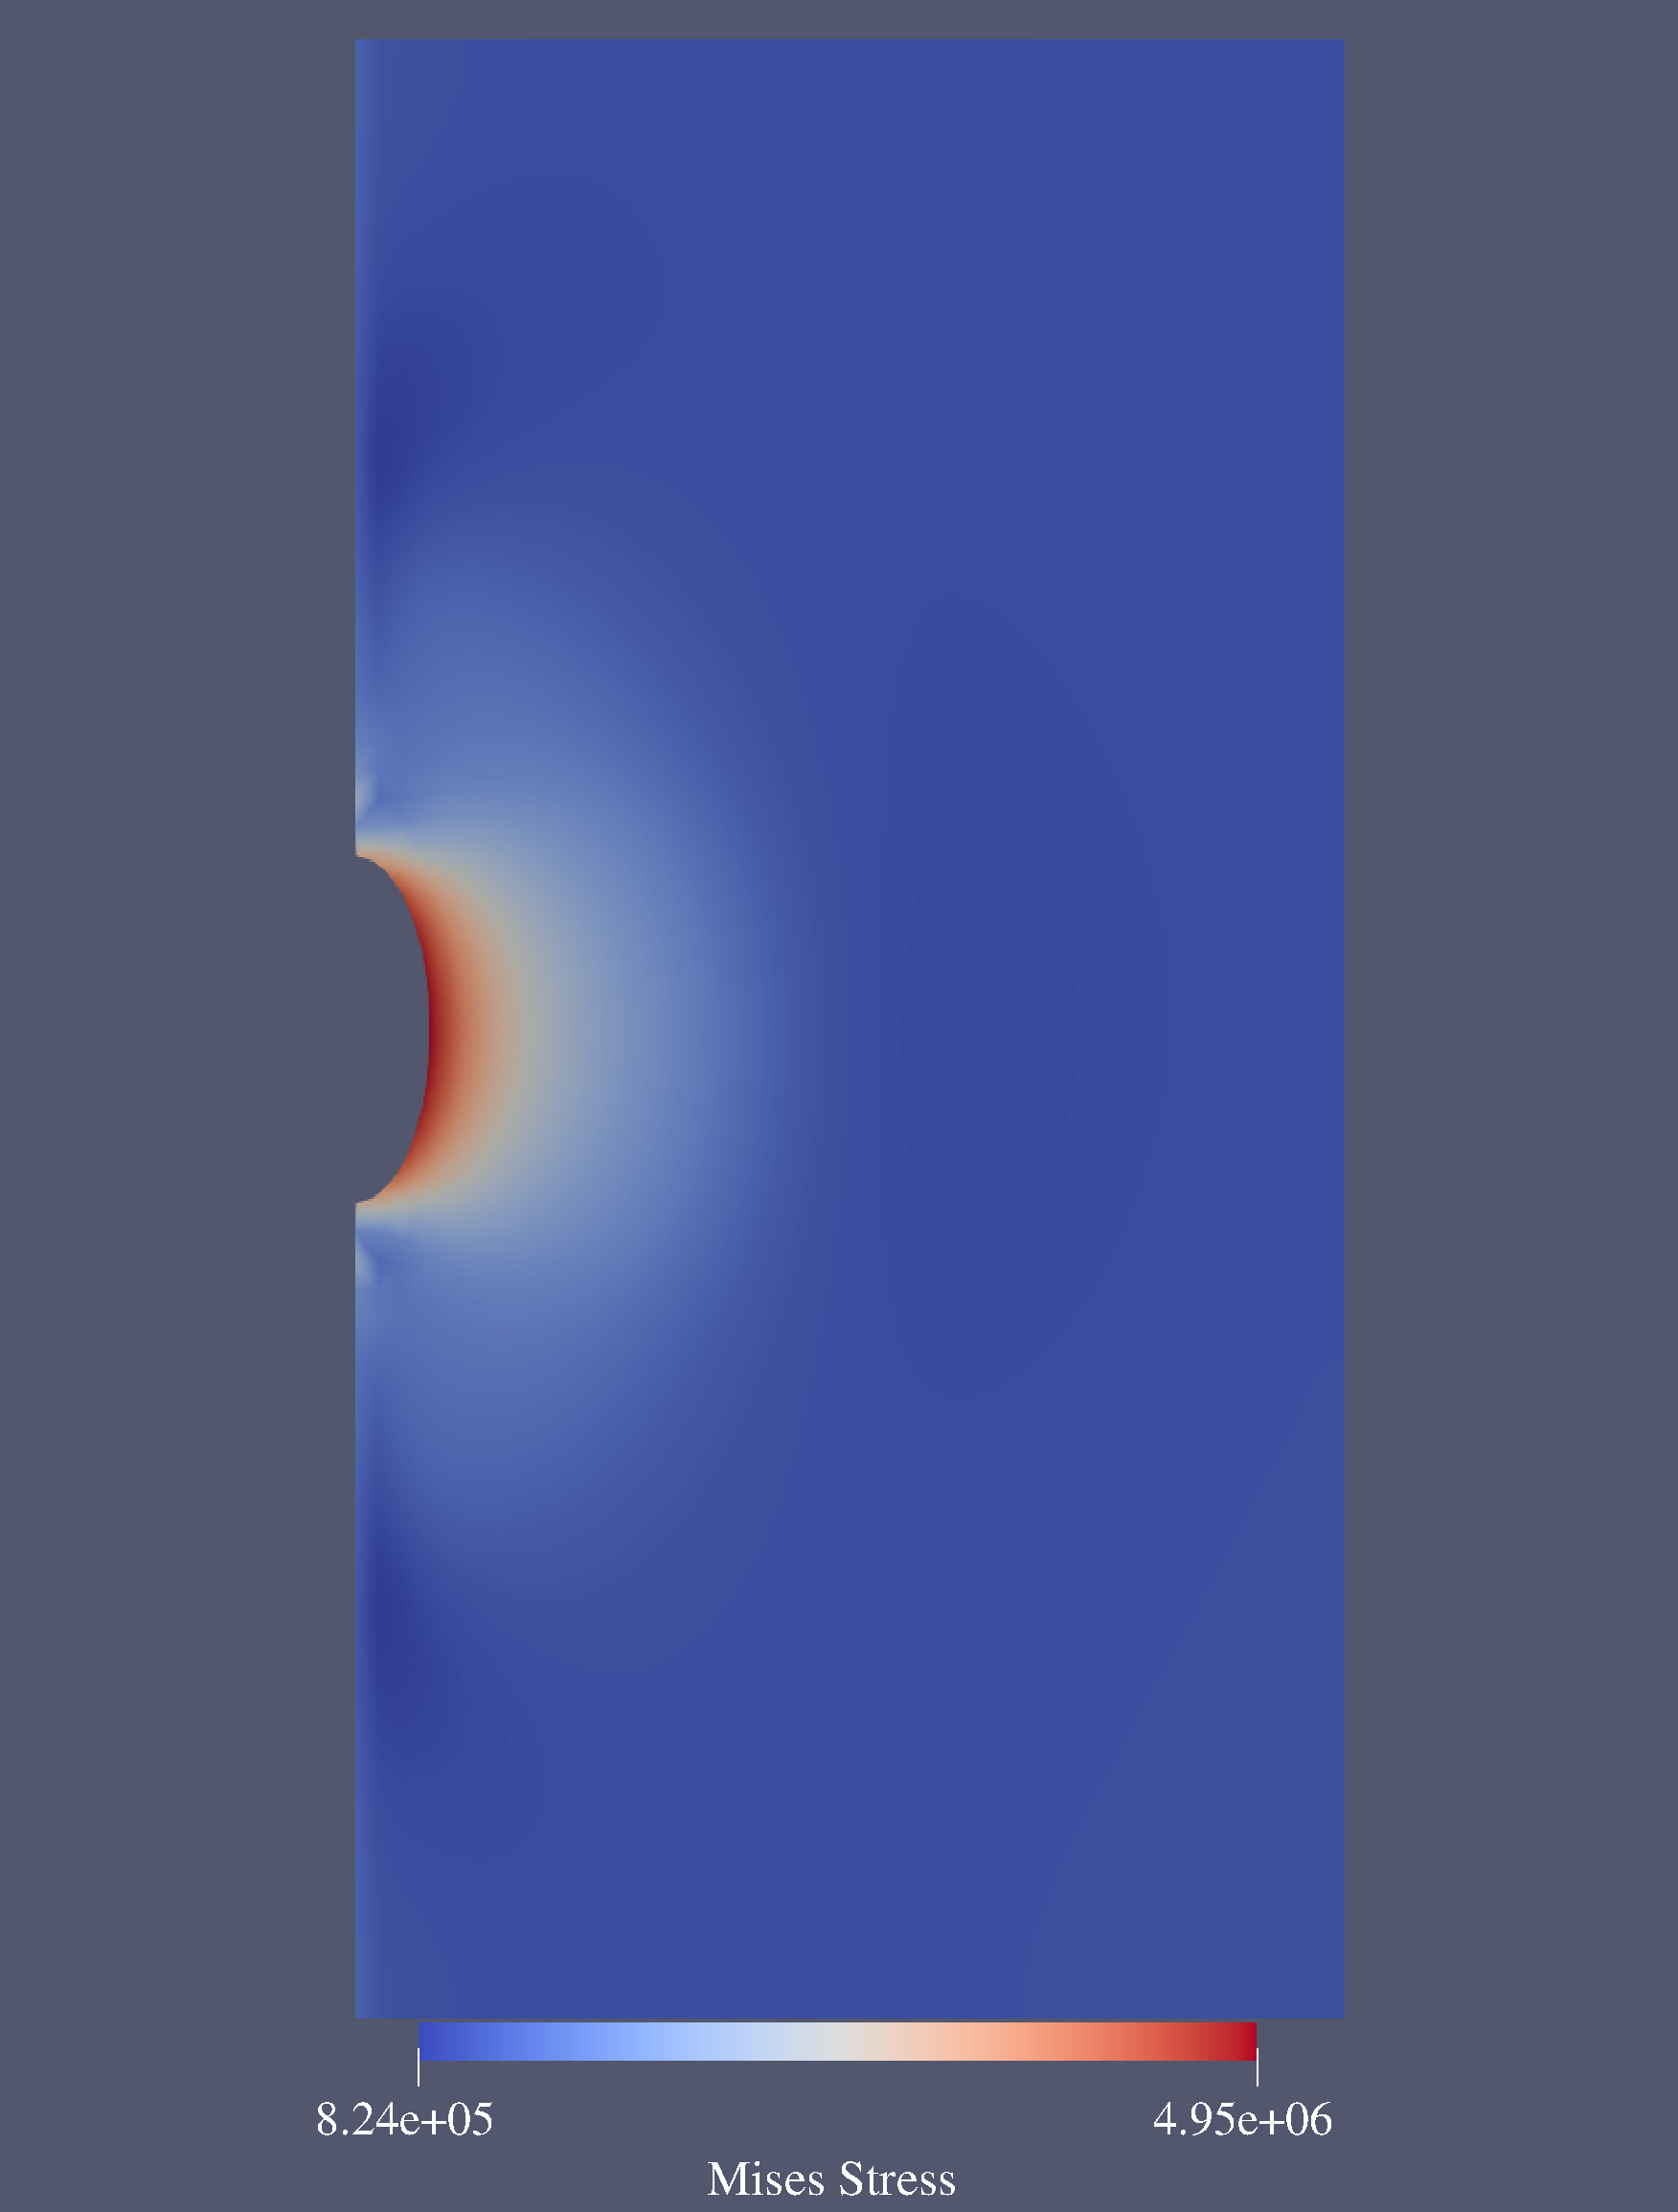
\includegraphics[width=0.95\textwidth]{img/chap5/应力/gk2mises.pdf}
        \end{minipage}
    }
    \subfigure[工况三运行\SI{10}{a}后Von Mises应力云图]
    {
        \begin{minipage}{7cm}
            \centering
            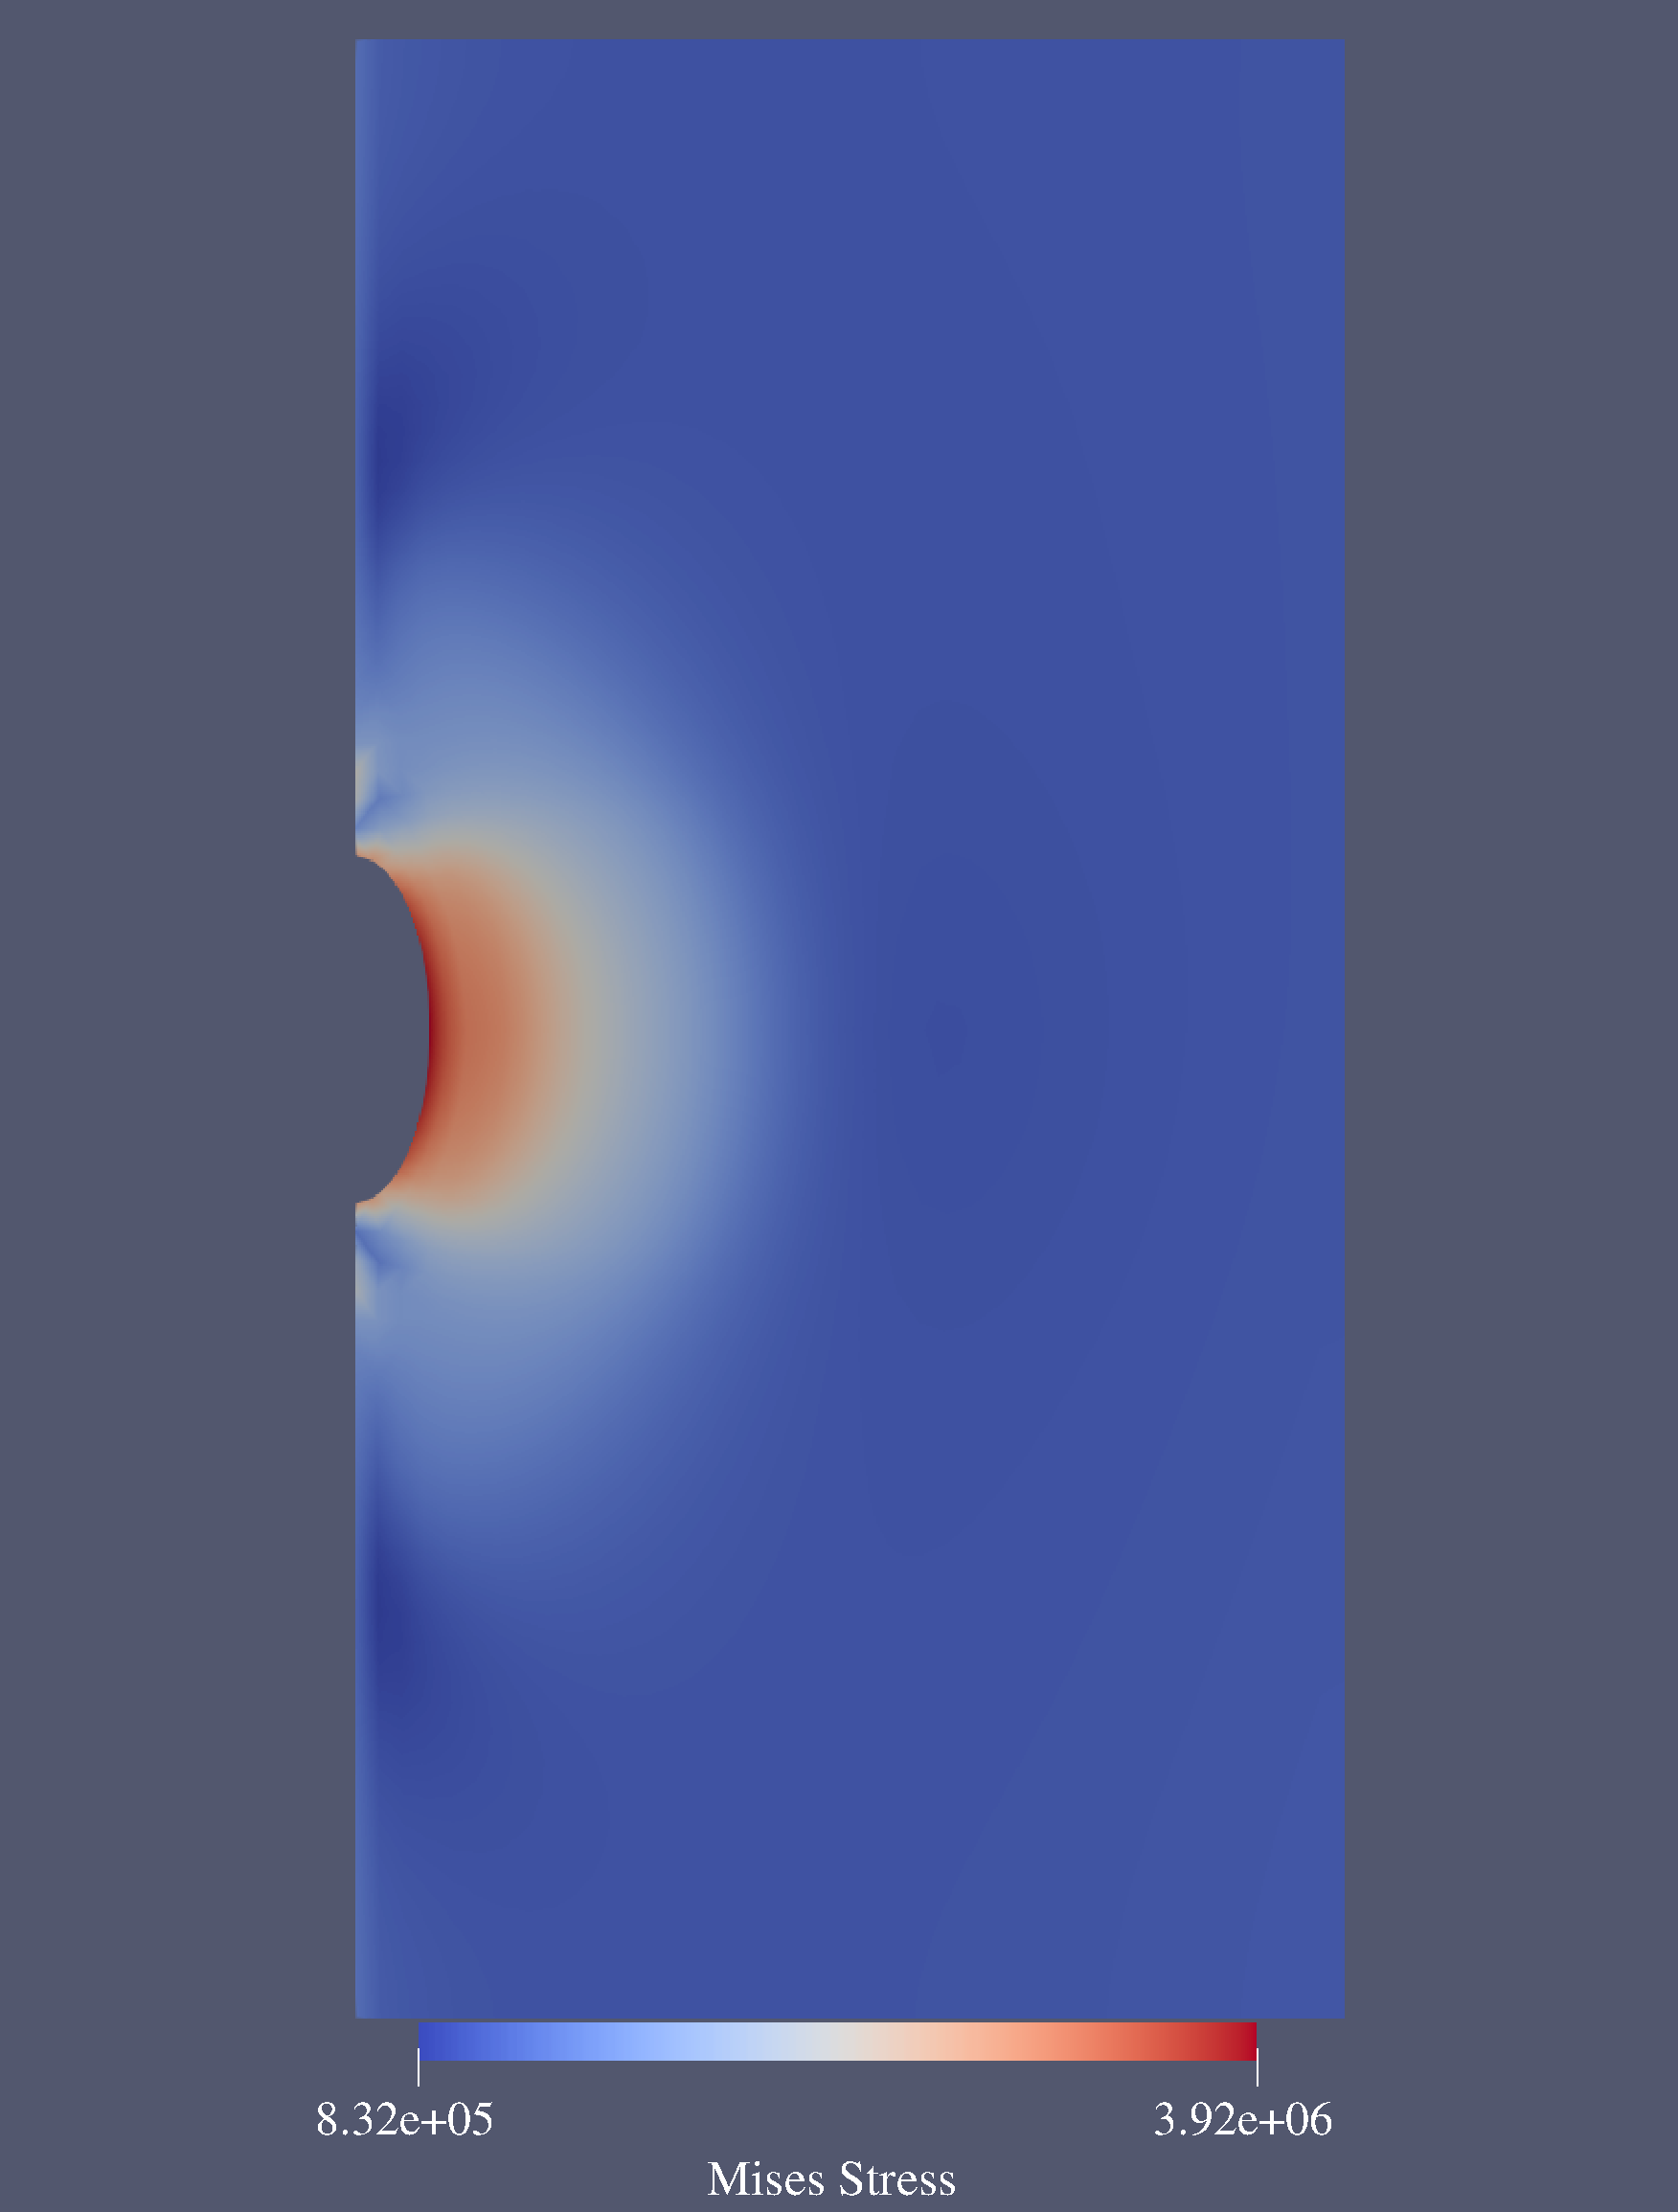
\includegraphics[width=0.95\textwidth]{img/chap5/应力/gk3mises.pdf}
        \end{minipage}
    } 
    \subfigure[工况四运行\SI{10}{a}后Von Mises应力云图]
    {
        \begin{minipage}{7cm}
            \centering
            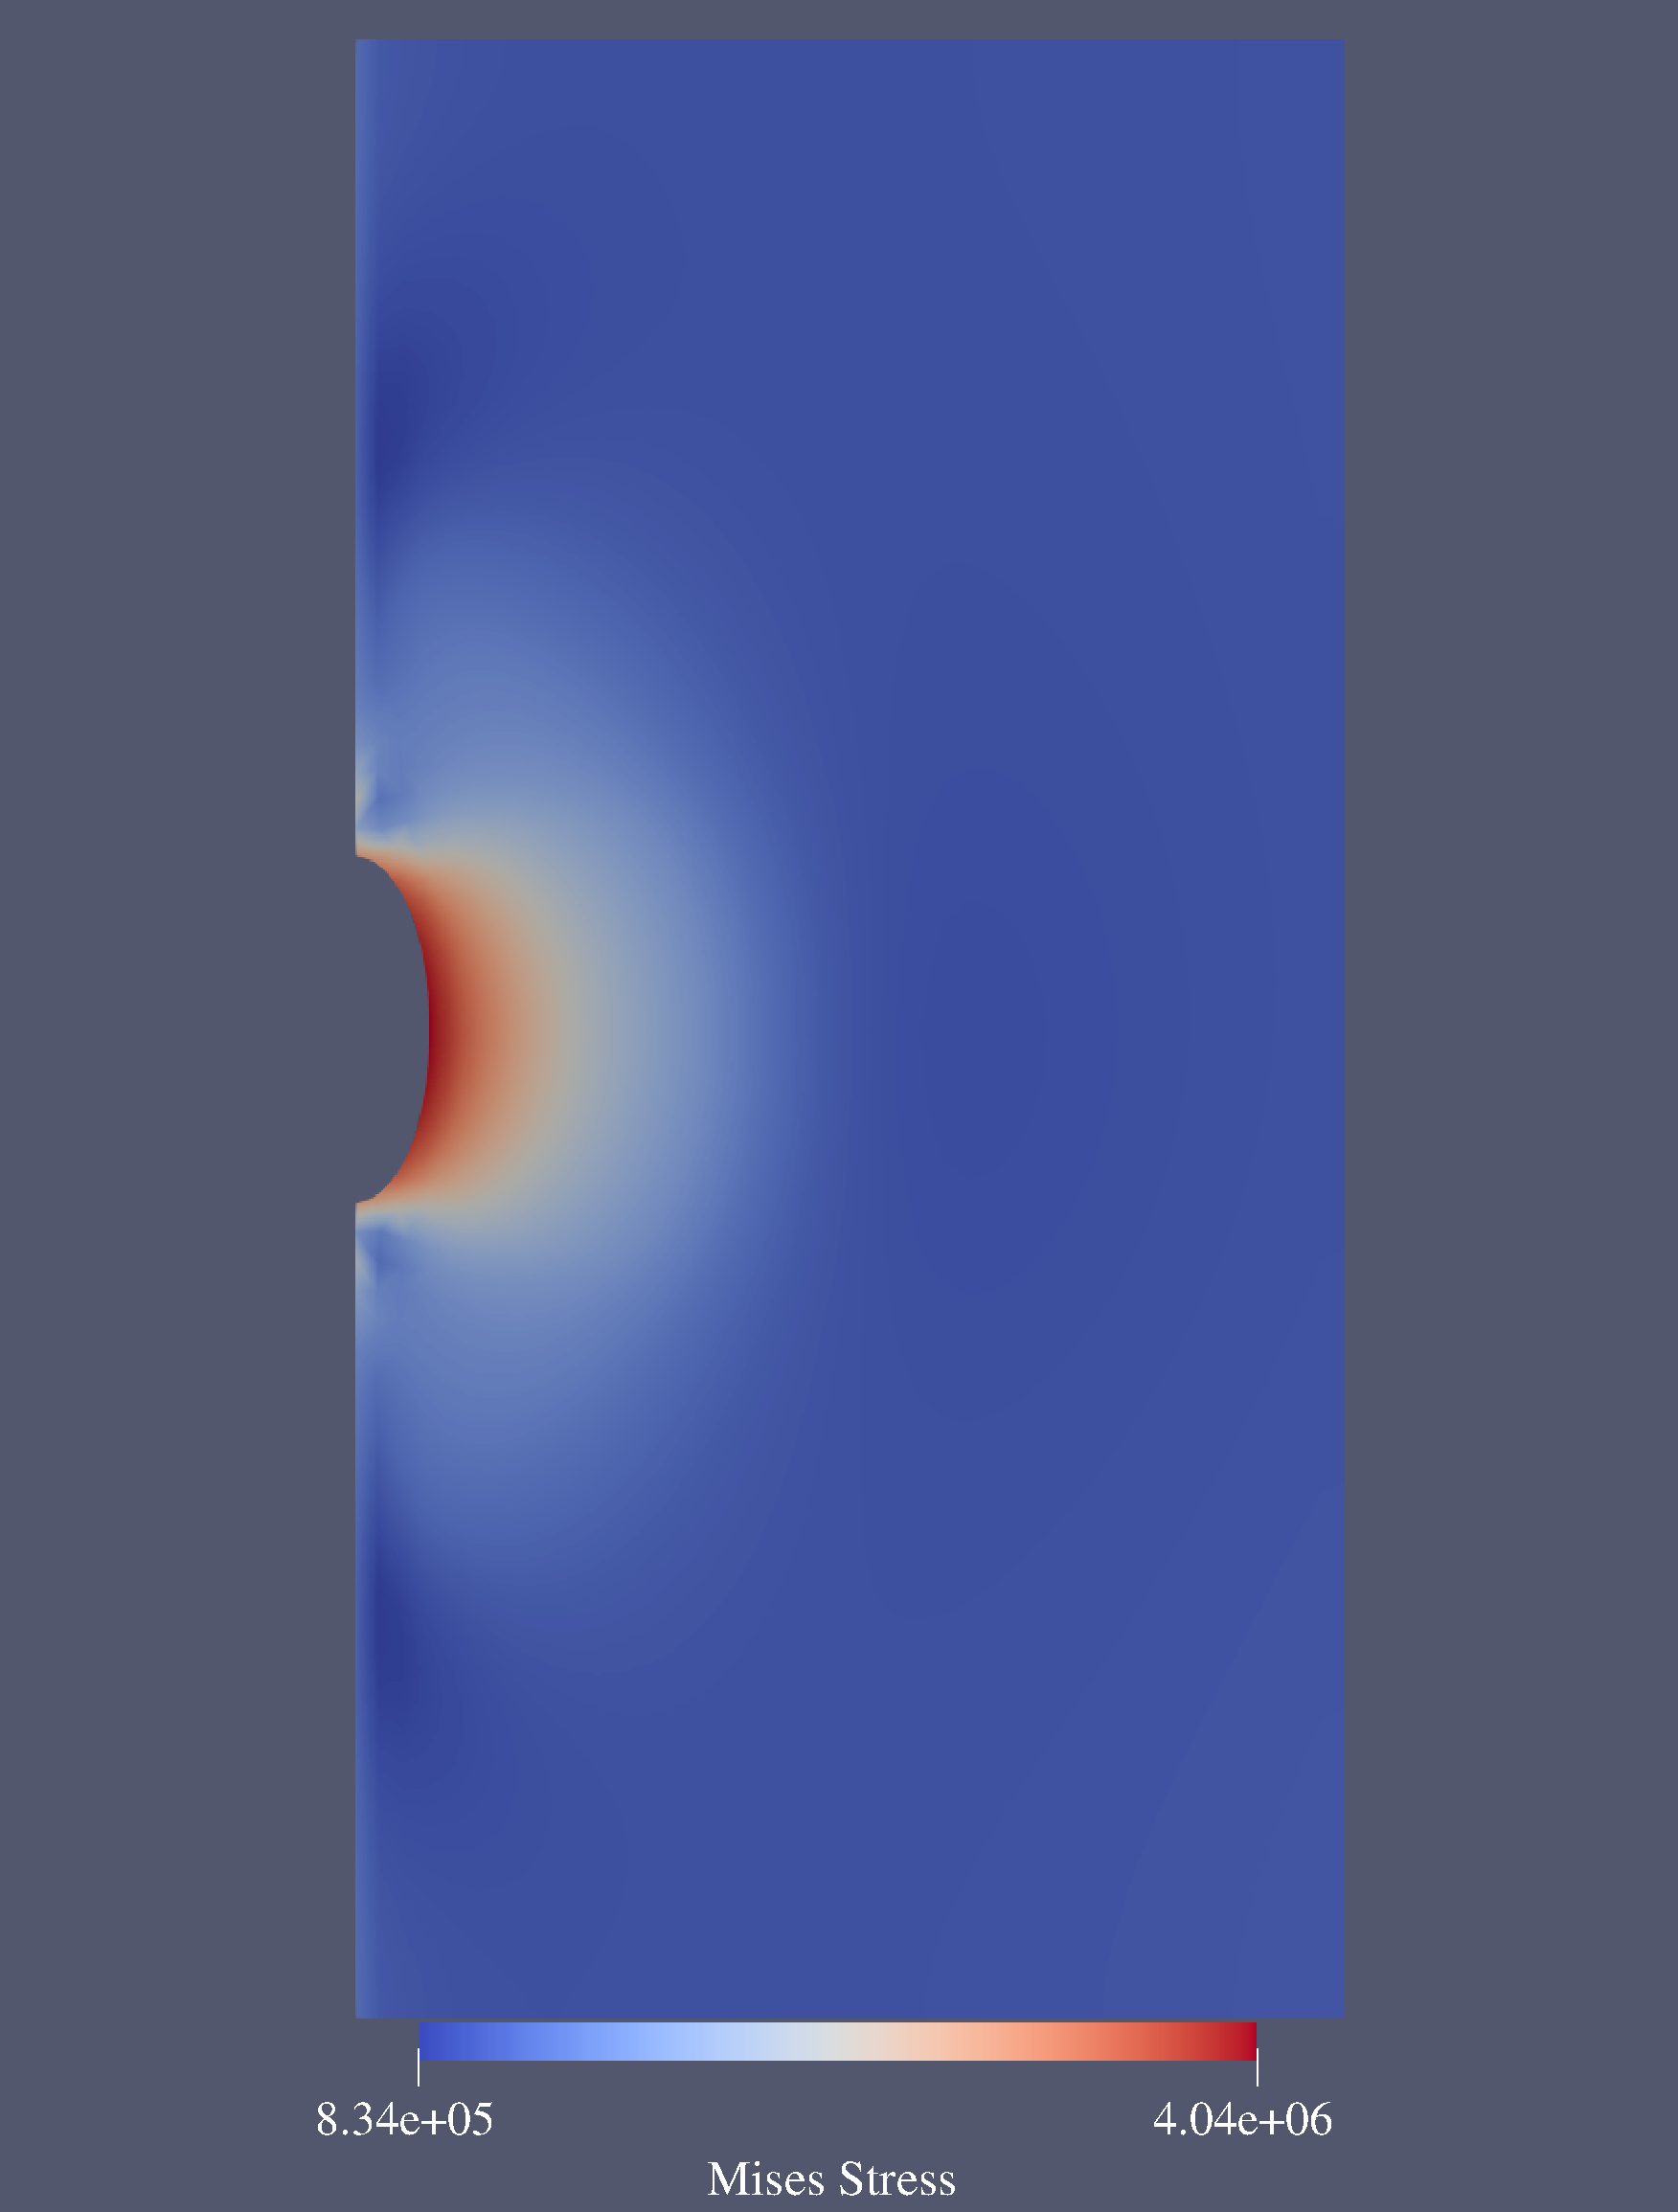
\includegraphics[width=0.95\textwidth]{img/chap5/应力/gk4mises.pdf}
        \end{minipage}
    }
    \caption{不同工况下运行\SI{10}{a}后Von Mises应力云图(单位:\si{Pa})}
    \label{fig:5_39}
\end{figure}

\begin{table}[ht!]\small
    \centering
    \begin{tabularx}{\textwidth}{C{1.0}C{1.0}C{1.0}C{1.0}}
        \toprule
        \multirow{2}{*}{计算工况} & \multicolumn{3}{c}{最大应力(MPa)}  \\
        \cmidrule(lr){2-4}
        \multicolumn{1}{c}{} &腔顶& 腔腰 & 腔底   \\
        \midrule
        工况一 &3.57    &4.78  &3.51 \\
        工况二  &3.33  &4.95  &3.19 \\ 
        工况三  &2.98  & 3.92 &2.97\\ 
        工况四 & 3.06   &4.04  &3.00 \\
        \bottomrule
    \end{tabularx}
    \caption{不同工况围岩中各位置最大Mises应力表(t=3650d)}
    \label{tab:5_10}
\end{table}

绘制各工况下各部分典型位置Mises应力与时间关系曲线,见图~\ref{fig:5_38}。由图可以看出,在溶腔开挖初期等效应力非常大,随着储库运行应力发生松弛,并迅速减小,在运行一年以后,Mises等效应力随着循环周期发生周期性变化,且变化范围基本保持不变。符合盐岩蠕变时,应力不变而应变增加的特点。

通过比较图(a)和图(b)、图(c)和图(d),即对比不同类型储库是否考虑热应力的曲线图,发现等效应力的大小变化不明显,说明是否考虑热力耦合对于围岩中应力的影响十分有限。通过比较图(a)和图(c)、图(b)和图(d),即对比不同类型储库长期运行下的等效应力大小,发现新能源储库中腔腰的等效应力明显大于腔顶和腔底部分,而传统能源储库三个不同位置的等效应力差距不明显。说明储库长期运行过程中,循环周期越短发生应力集中的现象越明显,关键部位的盐岩越容易发生破坏,从而影响储库的正常使用年限。

\begin{figure}[p]
    \centering
    \subfigure[工况一Mises应力与时间的关系曲线]
    {
        \begin{minipage}{7cm}
            \centering
            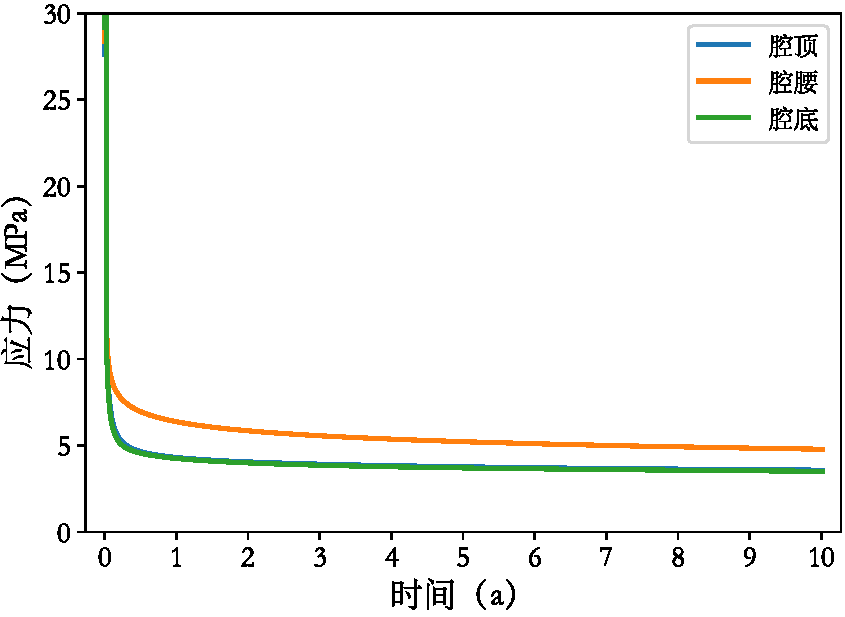
\includegraphics[width=0.95\textwidth]{img/chap5/应力/gk1mises_t.pdf}
        \end{minipage}
    }
      \subfigure[工况二Mises应力与时间的关系曲线]
    {
        \begin{minipage}{7cm}
            \centering
            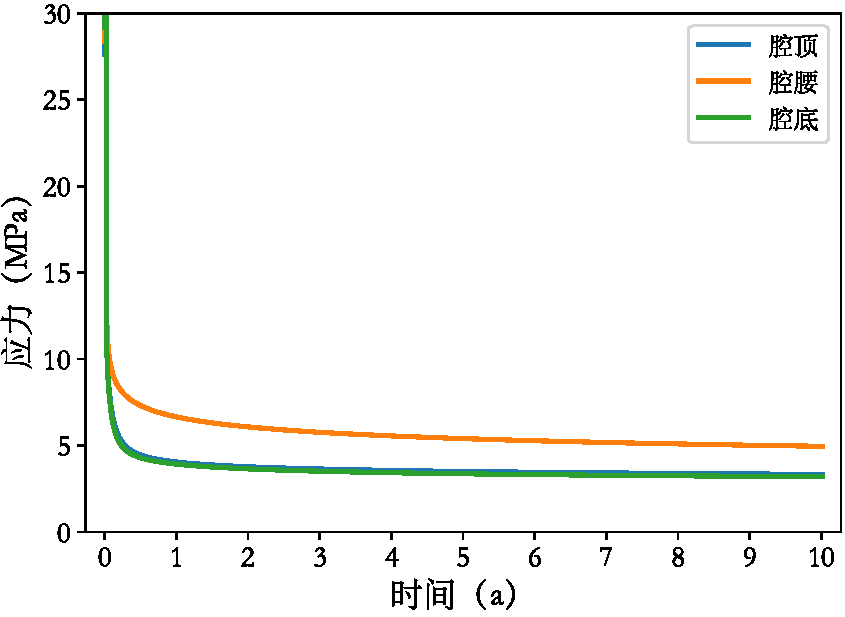
\includegraphics[width=0.95\textwidth]{img/chap5/应力/gk2mises_t.pdf}
        \end{minipage}
    }
    \subfigure[工况三Mises应力与时间的关系曲线]
    {
        \begin{minipage}{7cm}
            \centering
            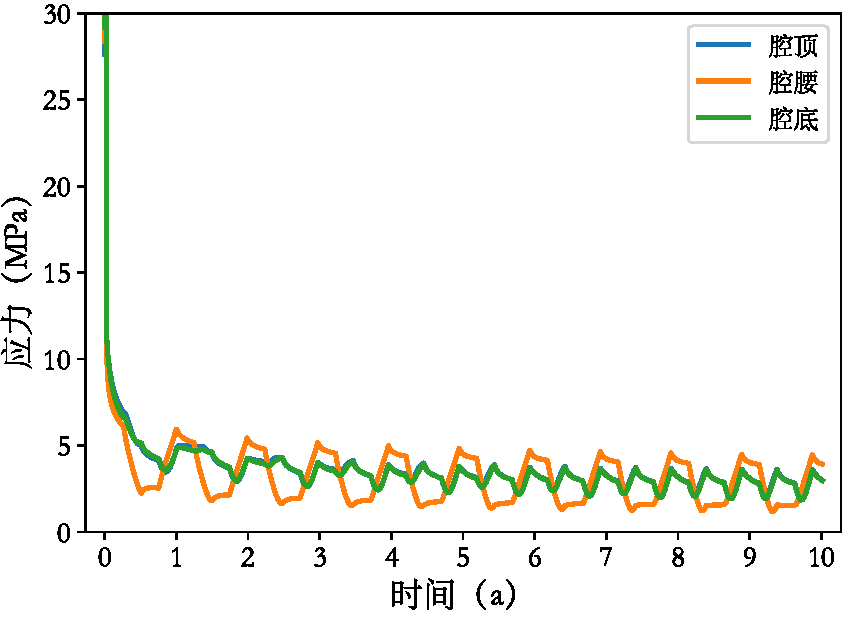
\includegraphics[width=0.95\textwidth]{img/chap5/应力/gk3mises_t.pdf}
        \end{minipage}
    } 
    \subfigure[工况四Mises应力与时间的关系曲线]
    {
        \begin{minipage}{7cm}
            \centering
            \includegraphics[width=0.95\textwidth]{img/chap5/应力/gk4mises_t.pdf}
        \end{minipage}
    }
    \caption{不同工况下运行\SI{10}{a}后典型位置Von Mises应力与时间的关系曲线(单位:\si{MPa})}
    %\vspace{128in}
    \label{fig:5_38}
\end{figure}

% \todoiZN{这里还没有整理完?还是分析不够的,要分析变力的变化规律,热应力是增加的,但是随着变形的增加,应力又是松弛的,可以追踪一个点或几个点的应力的变化,分析一下变化规律。}
% \todoiWCJ{这个没整理完 一是不太知道分析啥 二是paraview不知道怎么调出我想要的图 就先整理其他的了}

% \todoiZN{好的}
% \section{30天模拟运行结果分析}
% \subsection{位移}
% 如图\ref{fig:5-6}所示,为储气库\SI{30}{d}运行结束后位移云图。围岩整体位移特征与\SI{1}{d}模拟运行结果相同。\SI{30}{d}位移最大值为0.27m,相较于不考虑热力耦合时,30d最大位移为0.25m,增大了7%。如图\ref{fig:5-9}为\SI{30}{d}内位移最大值随时间变化曲线。腔顶部发生向下的位移,腔体中部和底部位移方向向上,整个腔体呈现收缩趋势。不同位置的位移大小与时间关系如图\ref{fig:5-15}所示,\SI{30}{d}内腔体腰部位移最大,其次是腔底底部,腔体顶部发生位移最小。腔体中部内压与地应力差值最大,因此发生流变最大。


% \begin{figure}[ht!]
%     \centering
%     \includegraphics[width=0.5\textwidth]{img/chap5/30d位移云图.png}
%     \caption{\SI{30}{d}模拟运行位移云图}
%     \label{fig:5-6}
% \end{figure}


% \begin{figure}[ht!]
%     \centering
%     \includegraphics[width=0.7\textwidth]{img/chap5/30d内位移最大值随时间的变化曲线图.png}
%     \caption{30d内位移最大值随时间的变化曲线}
%     \label{fig:5-9}
% \end{figure}


% \begin{figure}[ht!]
%     \centering
%     \includegraphics[width=0.7\textwidth]{img/chap5/30d内腔体不同位置最大位移与时间的关系曲线.png}
%     \caption{30d内腔体不同位置最大位移与时间的关系曲线}
%     \label{fig:5-15}
% \end{figure}
% \subsection{应力}
% 如图\ref{fig:5-8}所示为30d储库应力分布云图。由于应力梯度和椭圆形的腔体构造,应力主要集中在腔体顶部和腔体底部。底部最大应力为16.77MPa,顶部最大应力为14.90MPa。底部与顶部最大应力与时间关系如图\ref{fig:5-12}所示。
% \begin{figure}[ht!]
%     \centering
%     \includegraphics[width=0.7\textwidth]{img/chap5/顶部和底部应力变化.png}
%     \caption{顶部与底部最大应力与时间关系图}
%     \label{fig:5-12}
% \end{figure}


% \begin{figure}[ht!]
%     \centering
%     \includegraphics[width=0.5\textwidth]{img/chap5/30d应力分布云图.png}
%     \caption{30d模拟运行Mises应力云图}
%     \label{fig:5-8}
% \end{figure}

% \subsection{温度}
% 如图\ref{fig:5-10}所示为30天温度分布云图,可以看出腔体四周的约为3m厚的围岩温度明显上升,最高达到了343K,相比最初的298K上升十分明显。由图\ref{fig:5-11}围岩温度与时间的关系可以看出,温度在15d以后上升的速度明显减慢,且温度影响范围相较于溶腔的直径较小,由此可以合理推测,当储库运行达到20年时,温度的影响范围仍十分有限。但温度的变化对于流变的影响较大,需要增加模拟时长加以验证。

% \begin{figure}[ht!]
%     \centering
%     \includegraphics[width=0.5\textwidth]{img/chap5/30d温度分布云图.png}
%     \caption{30d模拟运行温度应力云图}
%     \label{fig:5-10}
% \end{figure}

% \begin{figure}[ht!]
%     \centering
%     \includegraphics[width=0.7\textwidth]{img/chap5/30d内温度最大值随时间的变化曲线图.png}
%     \caption{30d内温度最大值随时间的变化曲线图}
%     \label{fig:5-11}
% \end{figure}

% \begin{itemize}
%     \item 7d 2D
%     \item 2D vs 3D
% \end{itemize}


% \begin{itemize}
%     \item 无温度,战略储库
%     \item 有温度,战略储库(周期一年),共运营时间一样,5年
%     \item 有温度,新能源储库(周期一天),共运营时间一样,5年
% \end{itemize}

\section{小结}

本章在第四章的基础上,以江苏金坛盐矿为实例,建立计算模型。参考金坛盐矿储库的具体运作情况,及相关文献资料,结合不同类型储库的实际功能,从注采时长、内压变化、温度变化、循环周期四个方面制定了两种储库的不同运行工况,并根据工况编写了相应的OpenGeoSys循环边界代码。

通过三维模型的计算发现,代码可运行且模拟结果符合盐岩力学特征和蠕变规律,但在计算高效性上有所欠缺,因此将三维模型转化为二维进行模拟计算。通过数值模拟结果,从位移、温度、应力三个主要方面,对比新能源储库和传统能源储备库运行十年后的表现发现:(1)是否考虑热力耦合效应,对于储库的位移场、温度和应力场均有明显影响;(2)运行十年后,考虑热力耦合效应的新能源储库最大位移增大了6.6%,传统能源储库最大位移增大了5.6%,但新能源储库的最大位移为\SI{0.336}{m},小于传统能源储库的最大位移为\SI{0.375}{m}。由此可以说明,新能源储库对于热力耦合效应引起的流变更为明显,然而高频注采在一定程度上对围岩的整体流变有抑制作用;(3)注采过程中气体的温度向围岩深处均匀传播,新能源储库由于循环注采周期较短,相同工况下,围岩最高温度小于传统能源储备库;且两种储库的温度影响范围均小于溶腔短轴的两倍;(4)新能源储库的应力集中现象比传统能源储备库更为明显。
